\documentclass[12pt]{extarticle}
\usepackage[paperwidth=15in,paperheight=7.2in]{geometry}
\usepackage{amsmath}
\usepackage{hyperref}
\usepackage{multirow}
\usepackage{pdfpages}
\usepackage[utf8]{inputenc}
\title{Kaon mixing: chiral and continuum extrapolations}
\author{R Mukherjee}
\date{\today}
\begin{document}
\maketitle
\tableofcontents
\clearpage
\begin{figure}
\centering
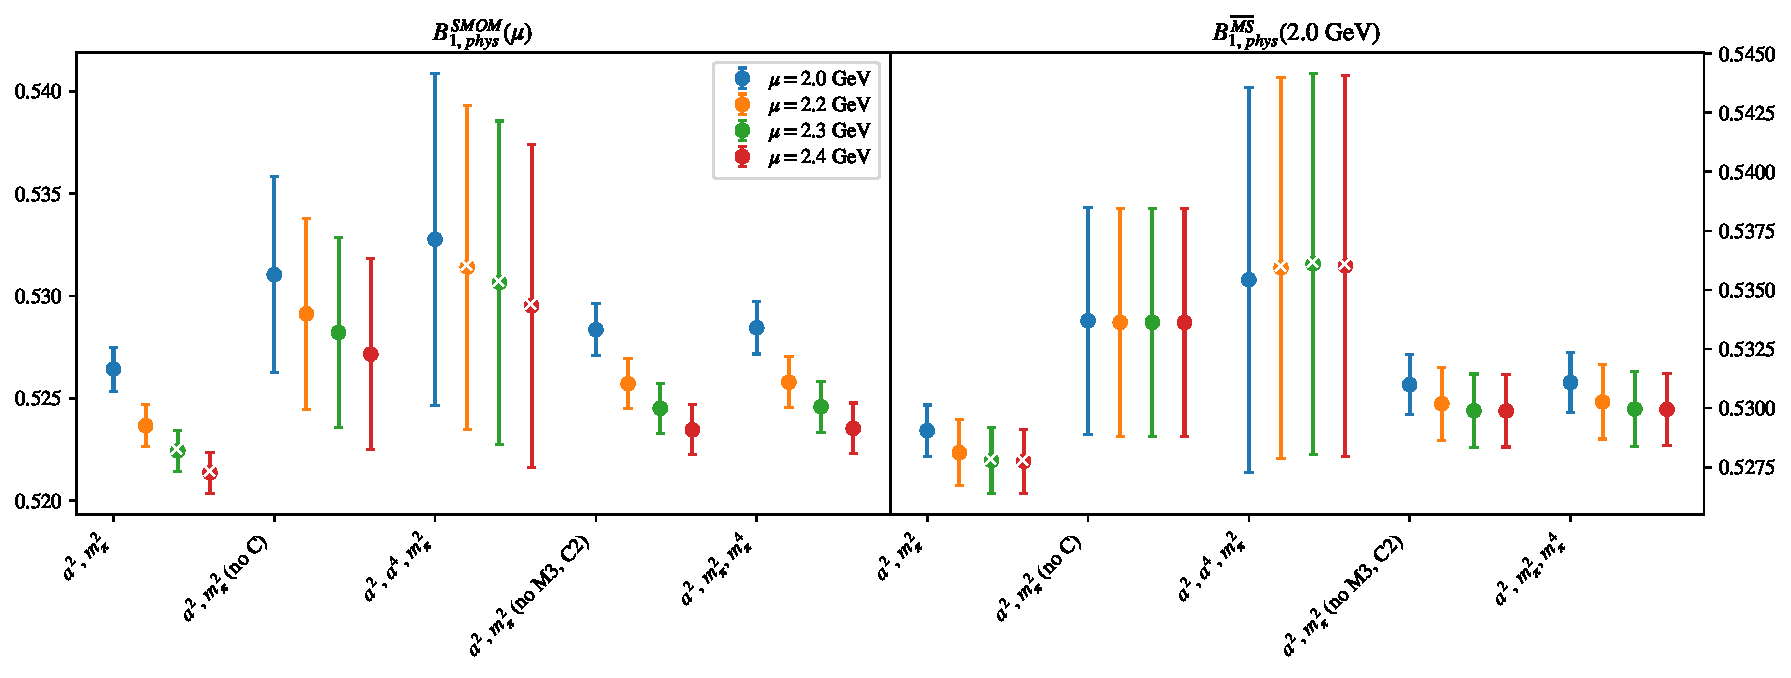
\includegraphics[page=1, width=1.1\textwidth]{VVpAA/NPR/fit_summary.pdf}
\caption{$B_{1}$\\(left) $B_{phys}$ in RI/SMOM scheme from fit variations (fits with $p$-value $<0.05$ marked with ``$\times$"). \\(right) $B_{phys}$ in $\overline{MS}$ computed using $B^{\overline{MS}} = R^{\overline{MS}\leftarrow SMOM}(2.0)\sigma_{npt}(2.0,\mu) B^{SMOM}(\mu)$.}
\end{figure}
\clearpage
\begin{figure}
\centering
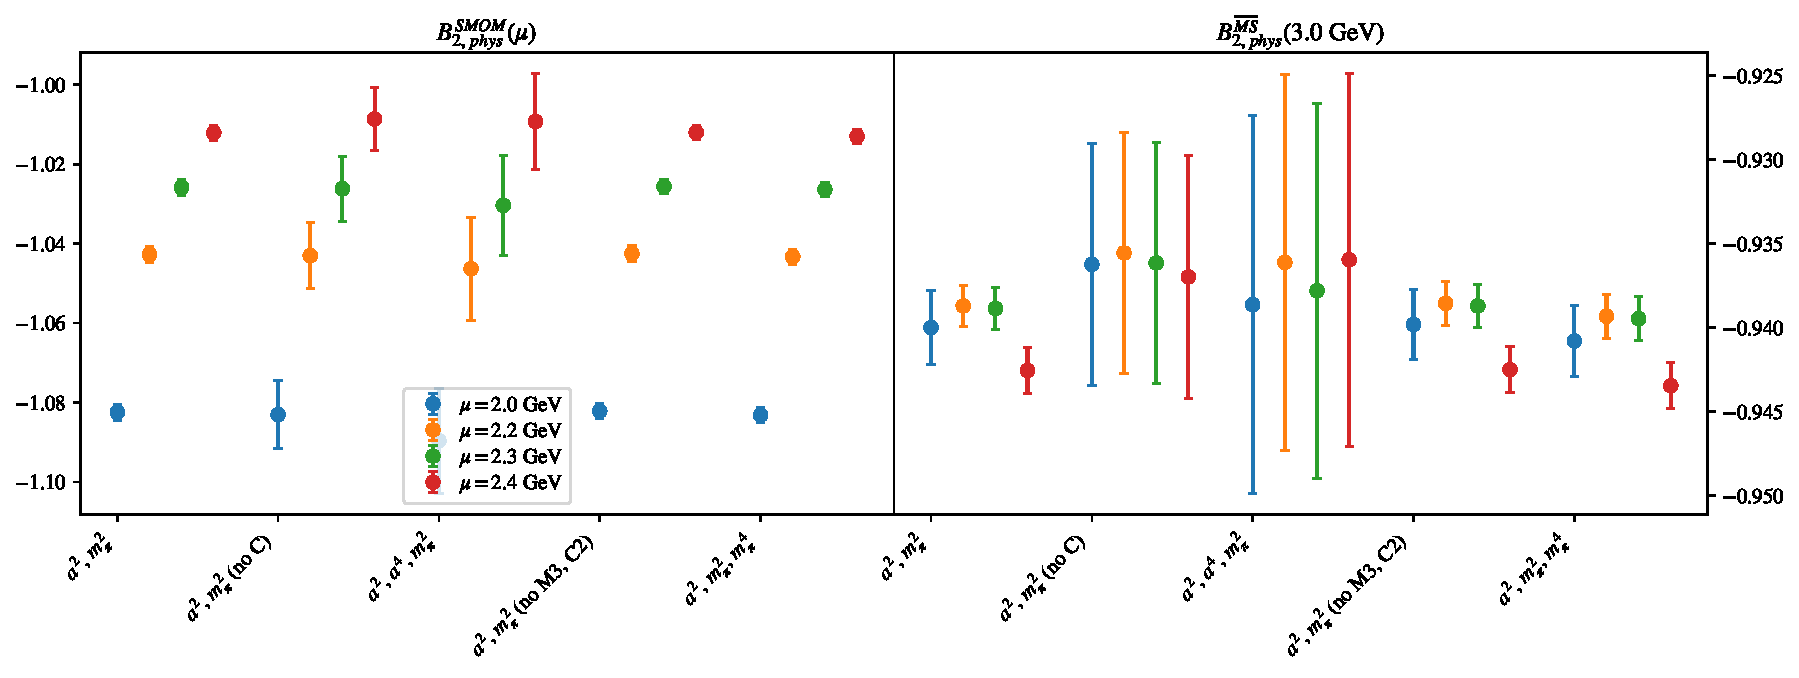
\includegraphics[page=1, width=1.1\textwidth]{VVmAA/NPR/fit_summary.pdf}
\caption{$B_{2}$\\(left) $B_{phys}$ in RI/SMOM scheme from fit variations (fits with $p$-value $<0.05$ marked with ``$\times$"). \\(right) $B_{phys}$ in $\overline{MS}$ computed using $B^{\overline{MS}} = R^{\overline{MS}\leftarrow SMOM}(3.0)\sigma_{npt}(3.0,\mu) B^{SMOM}(\mu)$.}
\end{figure}
\clearpage
\begin{figure}
\centering
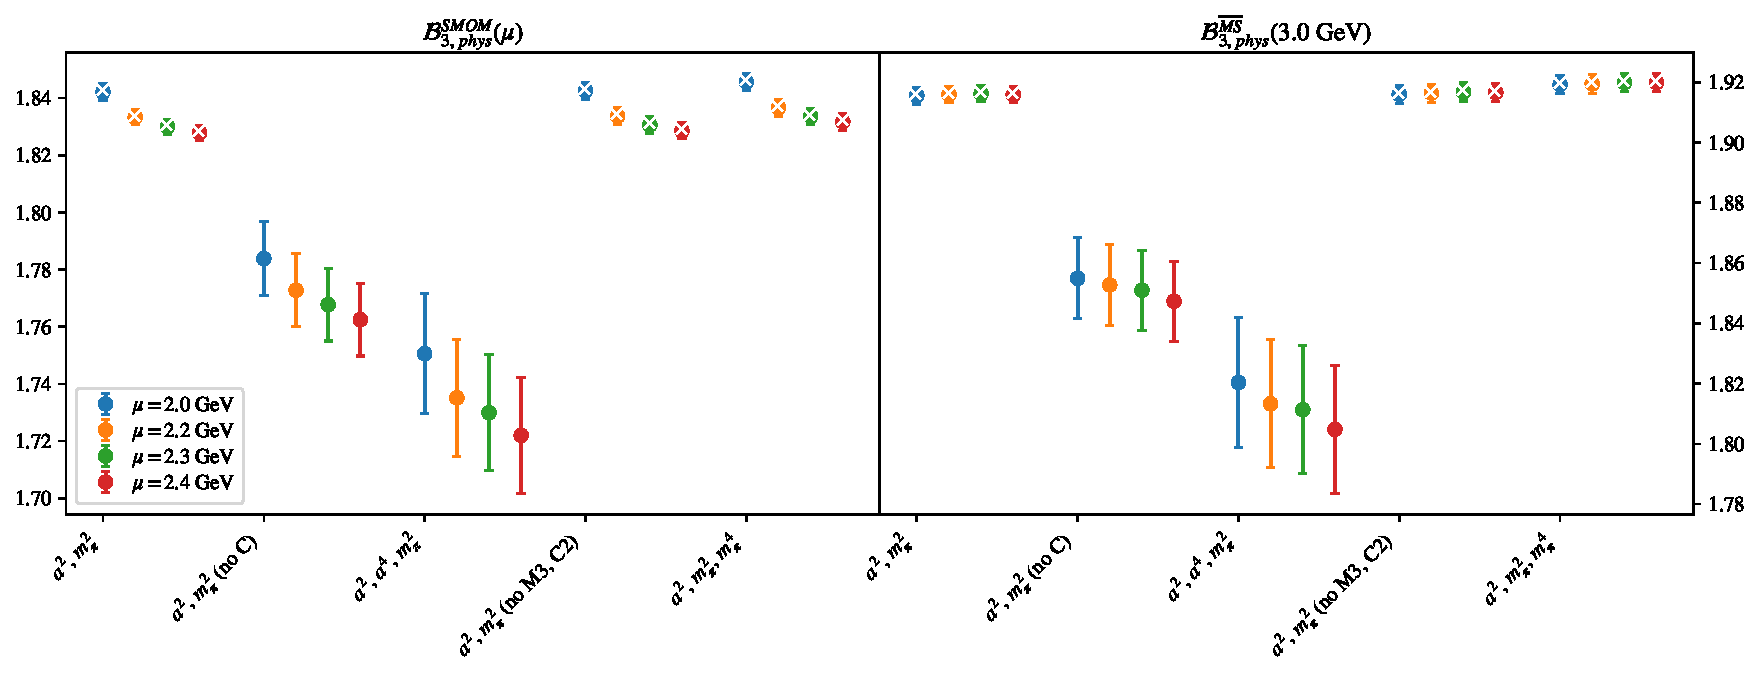
\includegraphics[page=1, width=1.1\textwidth]{SSmPP/NPR/fit_summary.pdf}
\caption{$B_{3}$\\(left) $B_{phys}$ in RI/SMOM scheme from fit variations (fits with $p$-value $<0.05$ marked with ``$\times$"). \\(right) $B_{phys}$ in $\overline{MS}$ computed using $B^{\overline{MS}} = R^{\overline{MS}\leftarrow SMOM}(3.0)\sigma_{npt}(3.0,\mu) B^{SMOM}(\mu)$.}
\end{figure}
\clearpage
\begin{figure}
\centering
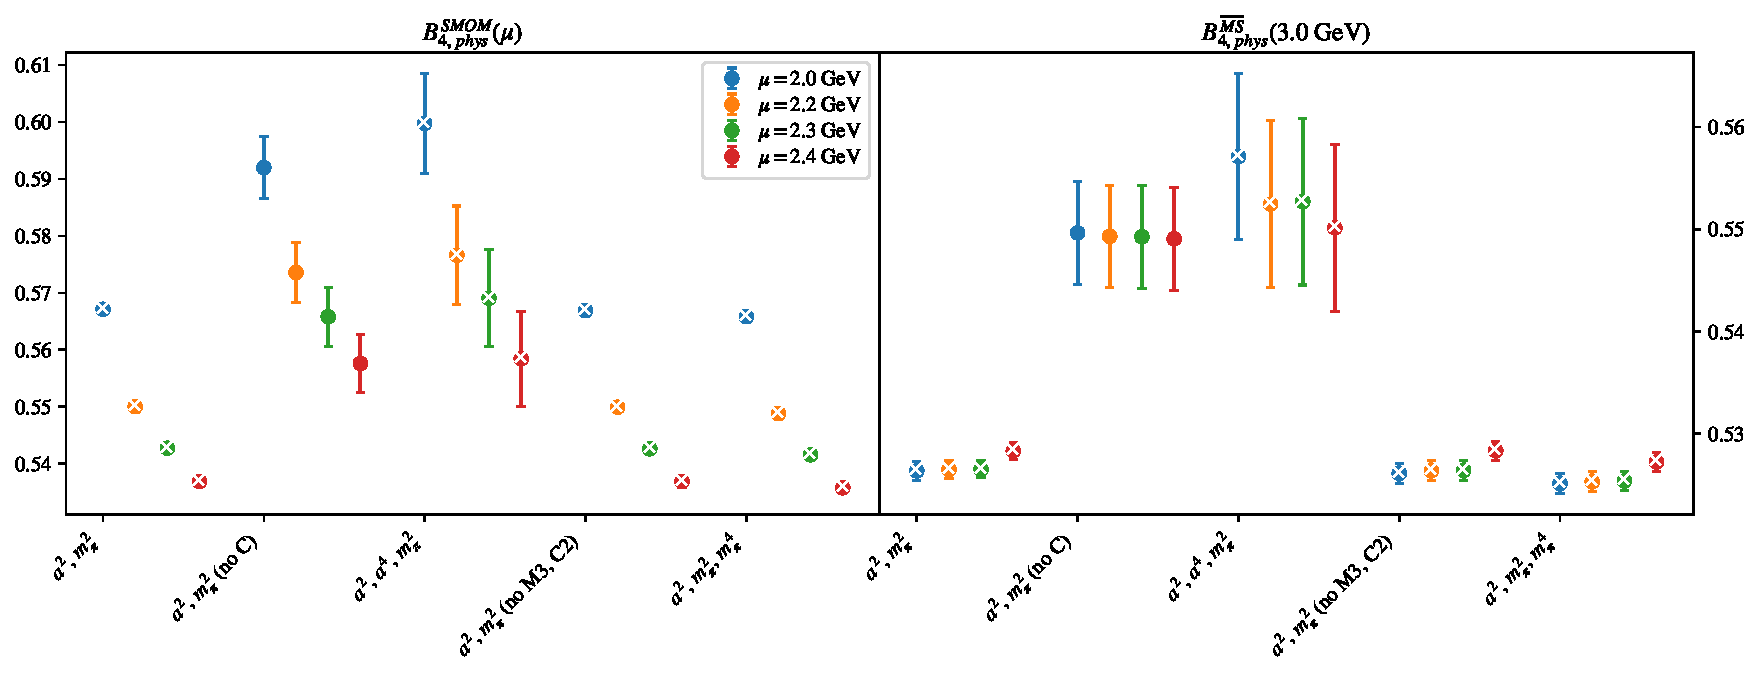
\includegraphics[page=1, width=1.1\textwidth]{SSpPP/NPR/fit_summary.pdf}
\caption{$B_{4}$\\(left) $B_{phys}$ in RI/SMOM scheme from fit variations (fits with $p$-value $<0.05$ marked with ``$\times$"). \\(right) $B_{phys}$ in $\overline{MS}$ computed using $B^{\overline{MS}} = R^{\overline{MS}\leftarrow SMOM}(3.0)\sigma_{npt}(3.0,\mu) B^{SMOM}(\mu)$.}
\end{figure}
\clearpage
\begin{figure}
\centering
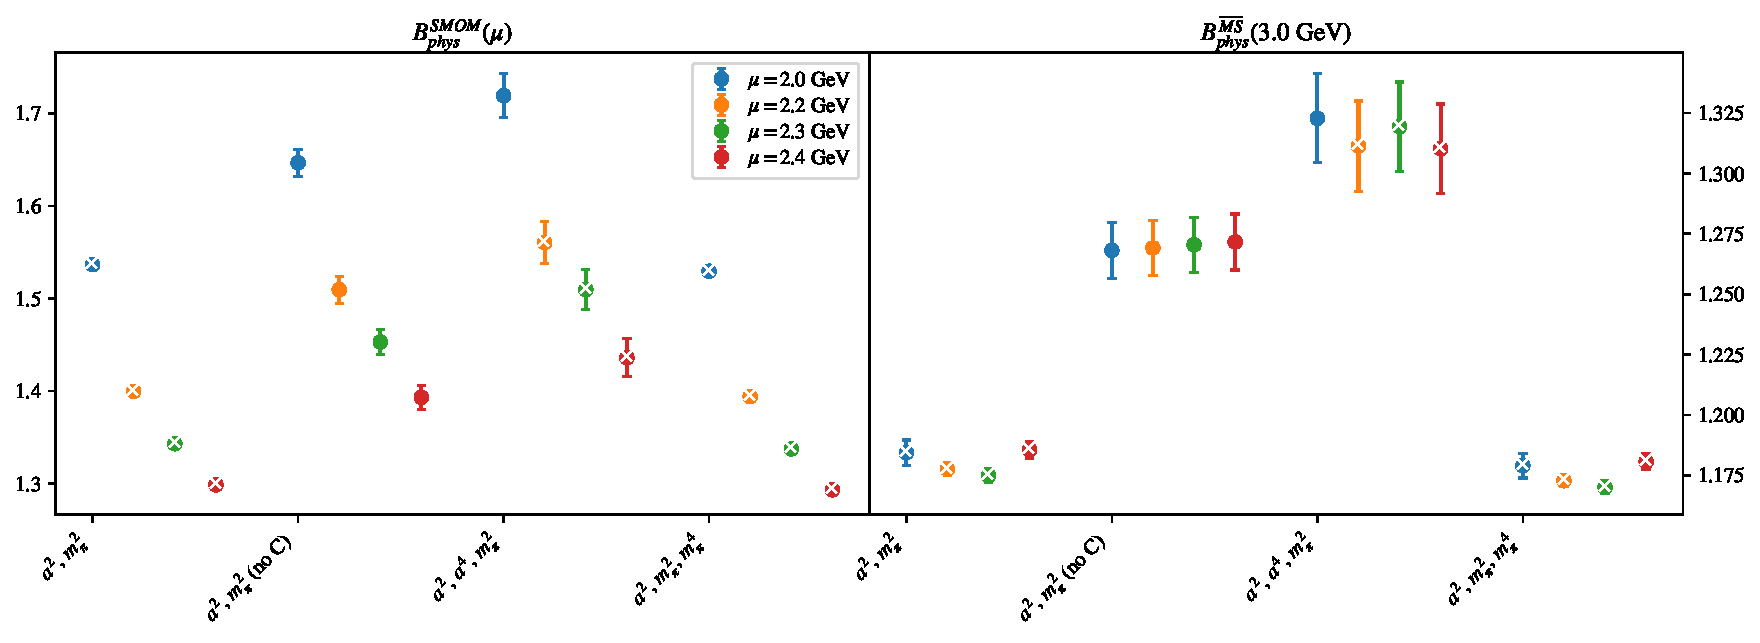
\includegraphics[page=1, width=1.1\textwidth]{TT/NPR/fit_summary.pdf}
\caption{$B_{5}$\\(left) $B_{phys}$ in RI/SMOM scheme from fit variations (fits with $p$-value $<0.05$ marked with ``$\times$"). \\(right) $B_{phys}$ in $\overline{MS}$ computed using $B^{\overline{MS}} = R^{\overline{MS}\leftarrow SMOM}(3.0)\sigma_{npt}(3.0,\mu) B^{SMOM}(\mu)$.}
\end{figure}
\clearpage
\section{$B_1$}
\begin{table}[h!]
\begin{center}
\begin{tabular}{|c|c|c|c|c|c|}
\hline
$\mu$ (GeV) & $a^2$, $m_\pi^2$& $a^2$, $m_\pi^2$ (no C)& $a^2$, $a^4$, $m_\pi^2$& $a^2$, $m_\pi^2$ (no M3, C2)& $a^2$, $m_\pi^2$, $m_\pi^4$\\
\hline
2.0& \hyperlink{VVpAA/NPR/a2m2_20.pdf.1}{\textbf{0.5264(10)}: 1.858 (0.098)} & \hyperlink{VVpAA/NPR/a2m2noC_20.pdf.1}{\textbf{0.5310(47)}: 0.876 (0.417)} & \hyperlink{VVpAA/NPR/a2a4m2_20.pdf.1}{\textbf{0.5327(81)}: 2.173 (0.069)} & \hyperlink{VVpAA/NPR/a2m2mcut_20.pdf.1}{\textbf{0.5283(12)}: 0.248 (0.863)} & \hyperlink{VVpAA/NPR/a2m2m4_20.pdf.1}{\textbf{0.5284(12)}: 0.661 (0.619)}\\
2.2& \hyperlink{VVpAA/NPR/a2m2_22.pdf.1}{\textbf{0.5236(10)}: 2.214 (0.05)} & \hyperlink{VVpAA/NPR/a2m2noC_22.pdf.1}{\textbf{0.5291(46)}: 1.143 (0.319)} & \hyperlink{VVpAA/NPR/a2a4m2_22.pdf.1}{\textbf{0.5314(79)}: 2.525 (0.039)} & \hyperlink{VVpAA/NPR/a2m2mcut_22.pdf.1}{\textbf{0.5257(12)}: 0.36 (0.782)} & \hyperlink{VVpAA/NPR/a2m2m4_22.pdf.1}{\textbf{0.5257(12)}: 0.923 (0.449)}\\
2.3& \hyperlink{VVpAA/NPR/a2m2_23.pdf.1}{\textbf{0.5224(10)}: 2.304 (0.042)} & \hyperlink{VVpAA/NPR/a2m2noC_23.pdf.1}{\textbf{0.5282(46)}: 1.197 (0.302)} & \hyperlink{VVpAA/NPR/a2a4m2_23.pdf.1}{\textbf{0.5306(78)}: 2.605 (0.034)} & \hyperlink{VVpAA/NPR/a2m2mcut_23.pdf.1}{\textbf{0.5245(12)}: 0.411 (0.745)} & \hyperlink{VVpAA/NPR/a2m2m4_23.pdf.1}{\textbf{0.5245(12)}: 0.993 (0.41)}\\
2.4& \hyperlink{VVpAA/NPR/a2m2_24.pdf.1}{\textbf{0.5213(10)}: 2.348 (0.039)} & \hyperlink{VVpAA/NPR/a2m2noC_24.pdf.1}{\textbf{0.5271(46)}: 1.223 (0.294)} & \hyperlink{VVpAA/NPR/a2a4m2_24.pdf.1}{\textbf{0.5295(78)}: 2.663 (0.031)} & \hyperlink{VVpAA/NPR/a2m2mcut_24.pdf.1}{\textbf{0.5234(12)}: 0.411 (0.745)} & \hyperlink{VVpAA/NPR/a2m2m4_24.pdf.1}{\textbf{0.5235(12)}: 1.005 (0.403)}\\
\hline
\end{tabular}
\caption{Physical point value from chiral and continuum extrapolation at renormalisation scale $\mu$. Entries are \textbf{value(error)}: $\chi^2/\text{DOF}$ ($p$-value).}
\end{center}
\end{table}
\begin{table}[h!]
\begin{center}
\begin{tabular}{|c c|c|c|c|c|c|}
\hline
$\mu$ (GeV) &  & $a^2$, $m_\pi^2$& $a^2$, $m_\pi^2$ (no C)& $a^2$, $a^4$, $m_\pi^2$& $a^2$, $m_\pi^2$ (no M3, C2)& $a^2$, $m_\pi^2$, $m_\pi^4$\\
\hline
\multirow{2}{0.5in}{2.0} & $\alpha$ & 0.0937(71)& 0.047(53)& -0.017& 0.0815(83)& 0.0813(82)\\
 & $\beta$ & 0.00261(14)& 0.00223(27)& 0.00263(15)& 0.00189(28)& 0.00031(90)\\
\hline
\multirow{2}{0.5in}{2.2} & $\alpha$ & 0.0977(70)& 0.041(52)& -0.038& 0.0847(83)& 0.0846(82)\\
 & $\beta$ & 0.00261(14)& 0.00220(27)& 0.00264(14)& 0.00184(28)& 0.00020(89)\\
\hline
\multirow{2}{0.5in}{2.3} & $\alpha$ & 0.0992(70)& 0.039(52)& -0.045& 0.0859(83)& 0.0859(82)\\
 & $\beta$ & 0.00262(14)& 0.00220(27)& 0.00265(14)& 0.00184(28)& 0.00018(89)\\
\hline
\multirow{2}{0.5in}{2.4} & $\alpha$ & 0.0999(70)& 0.040(52)& -0.044& 0.0864(83)& 0.0864(82)\\
 & $\beta$ & 0.00263(14)& 0.00220(27)& 0.00266(14)& 0.00184(28)& 0.00017(89)\\
\hline
\end{tabular}
\caption{Fit values of coefficients in $B = B_{phys} + \mathbf{\alpha} a^2 + \mathbf{\beta}\left(\frac{m_\pi^2}{f_\pi^2}-\frac{m_{\pi,PDG}^2}{f_\pi^2}\right) + \ldots$.}
\end{center}
\end{table}
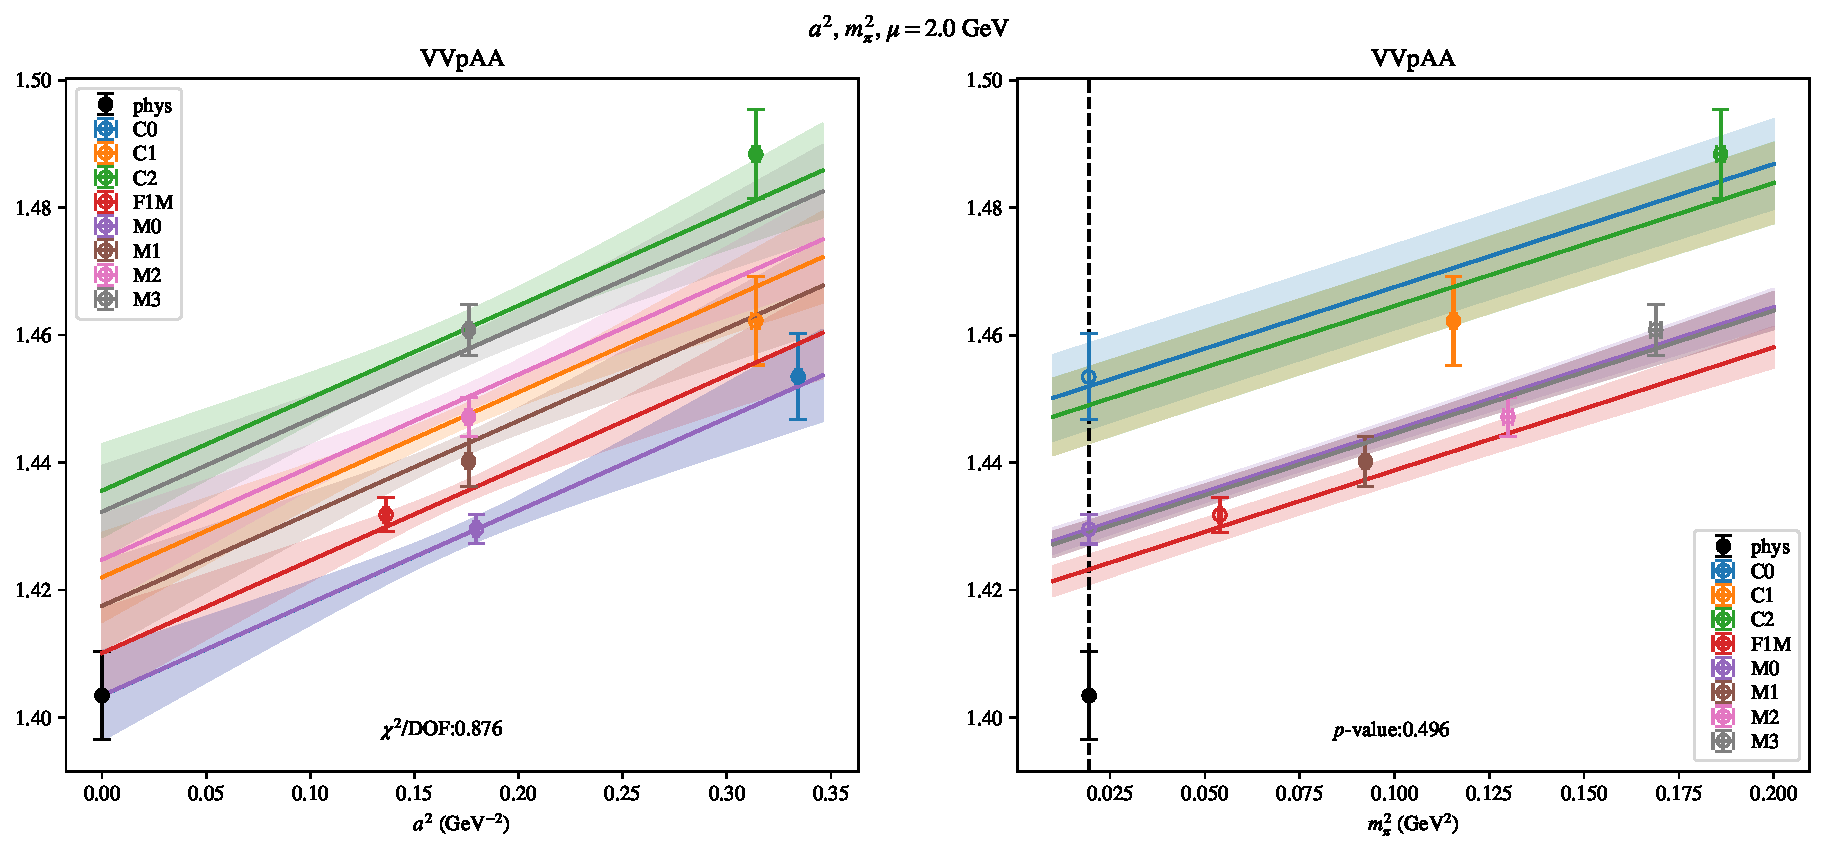
\includepdf[link, pages=-]{VVpAA/NPR/a2m2_20.pdf}
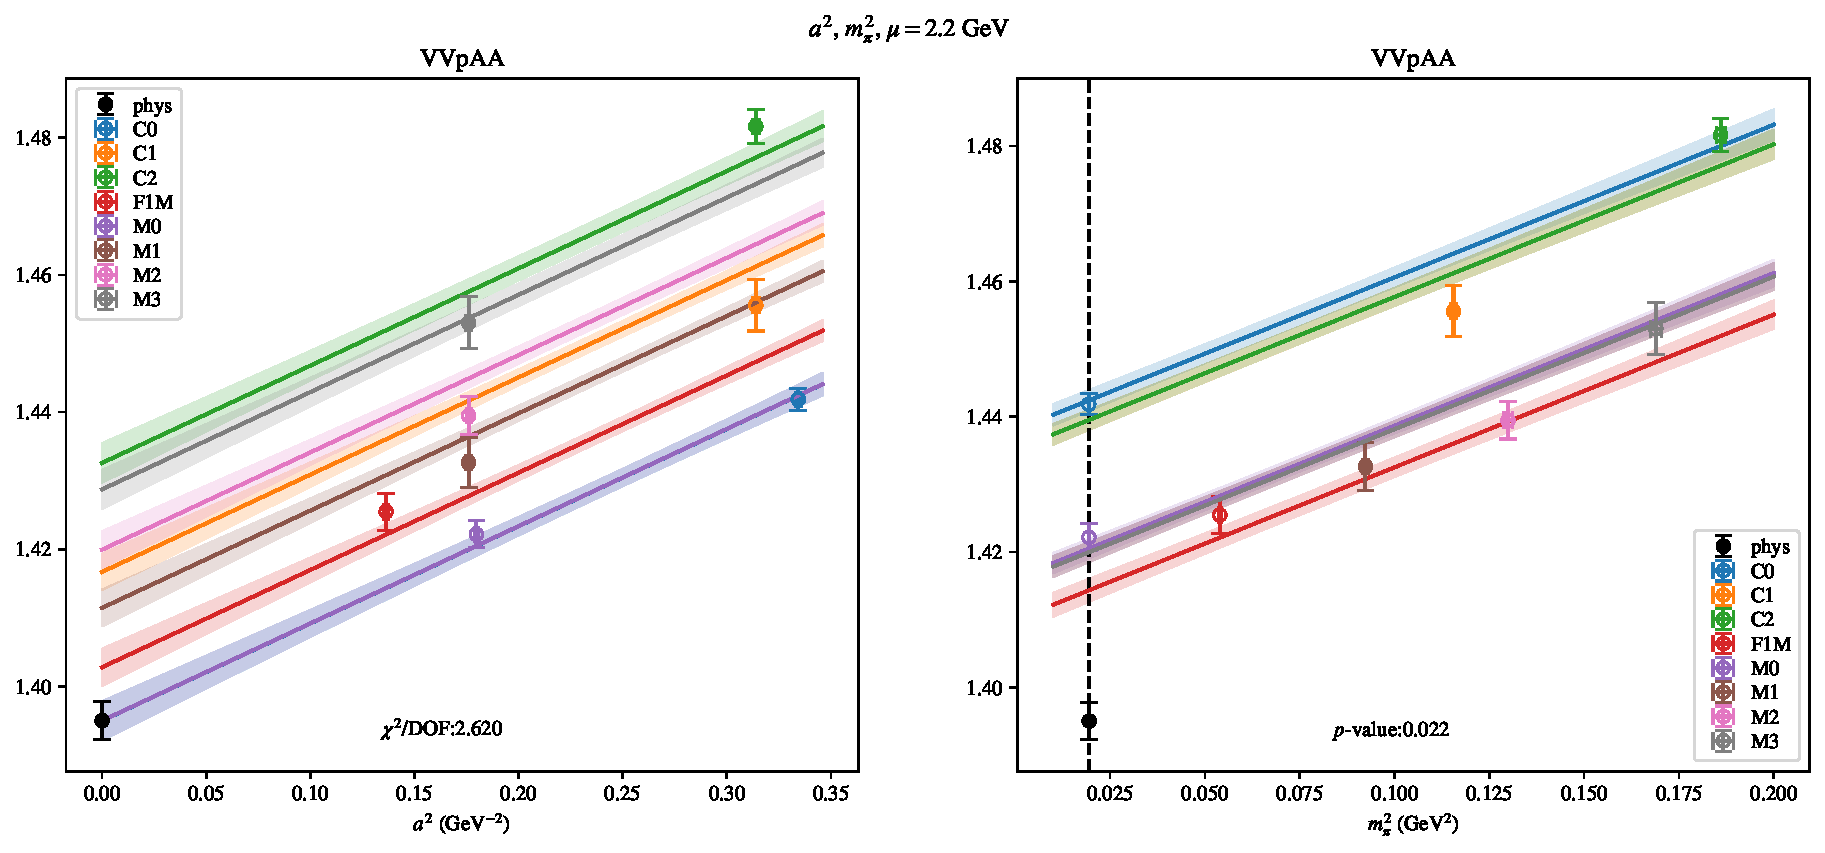
\includepdf[link, pages=-]{VVpAA/NPR/a2m2_22.pdf}
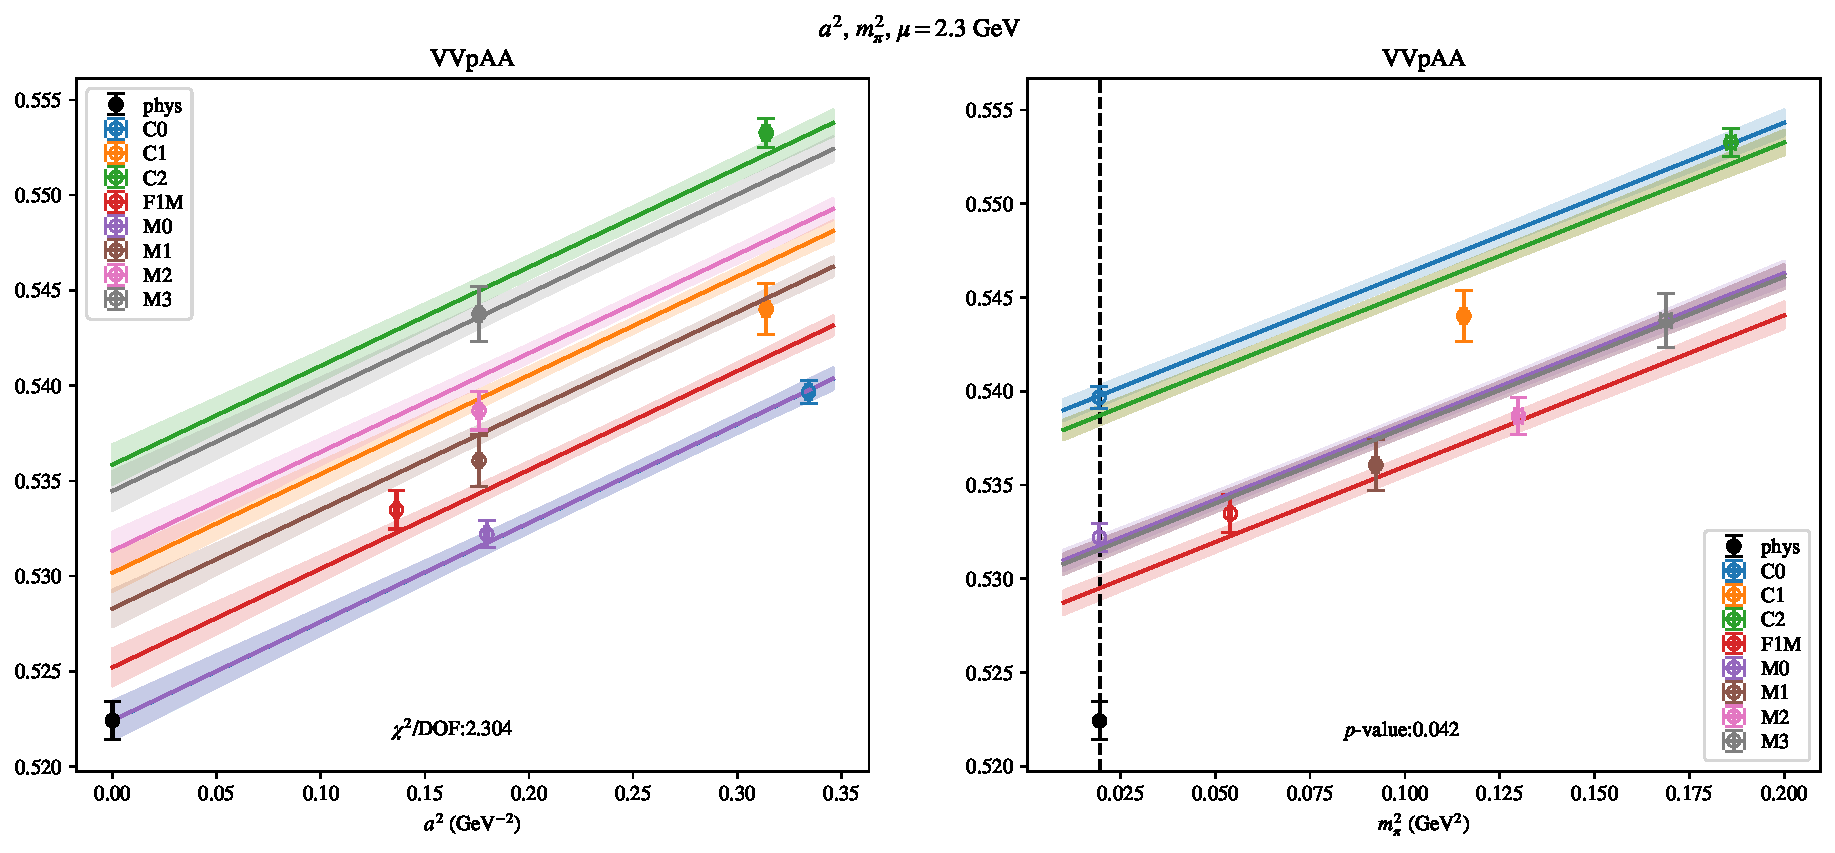
\includepdf[link, pages=-]{VVpAA/NPR/a2m2_23.pdf}
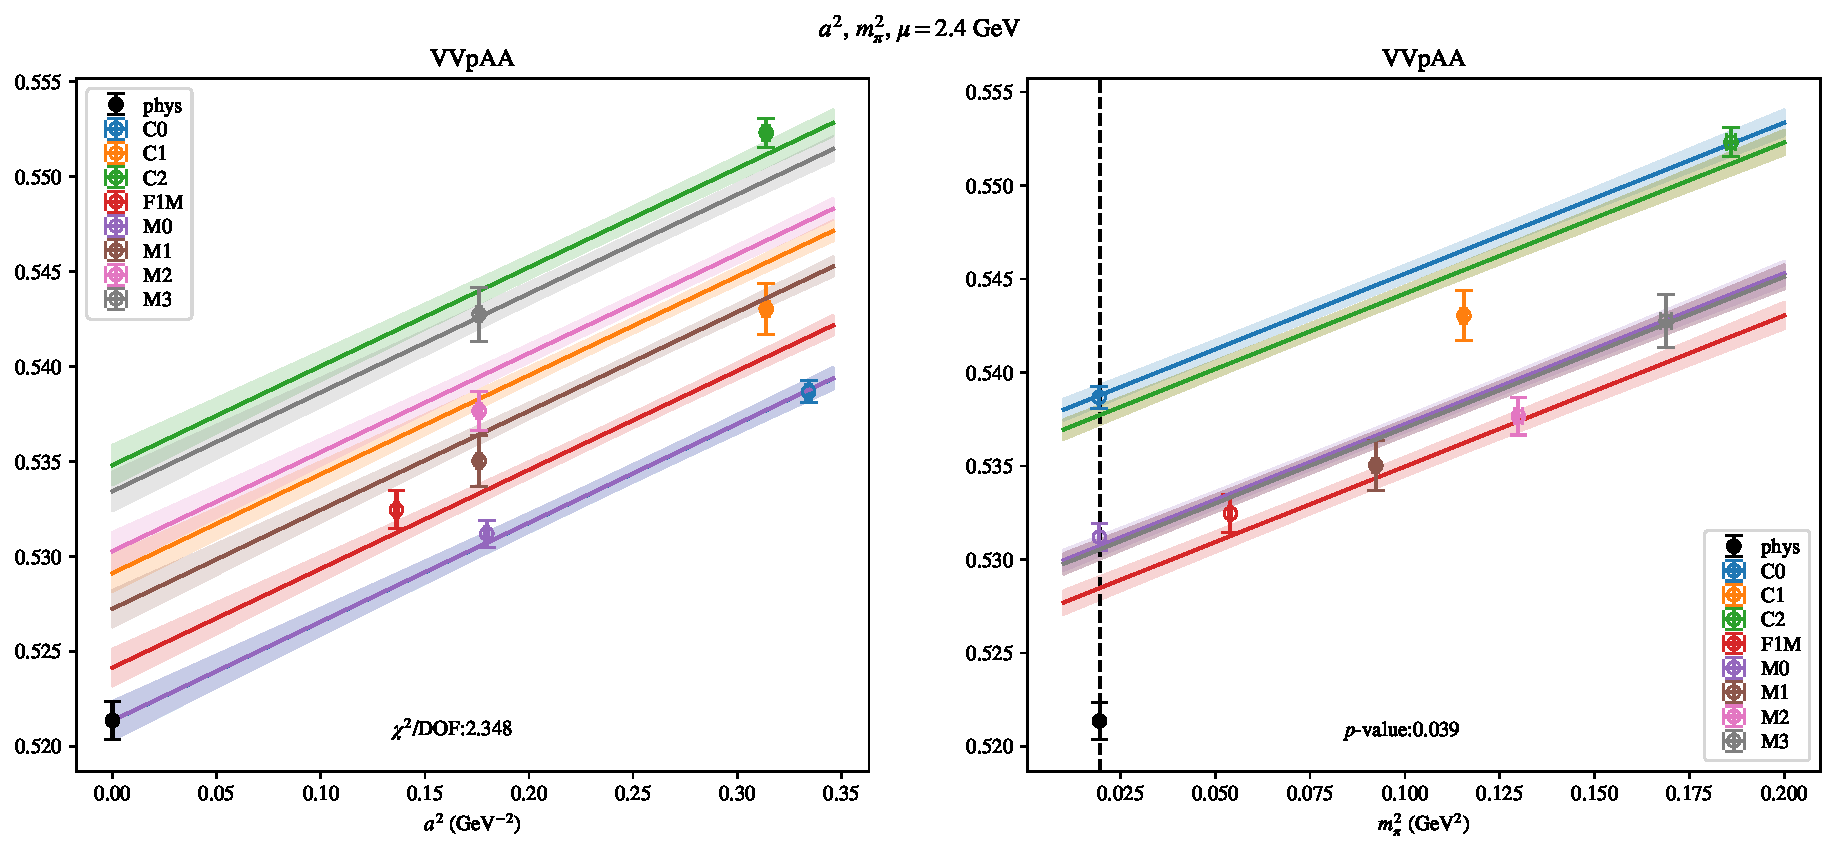
\includepdf[link, pages=-]{VVpAA/NPR/a2m2_24.pdf}
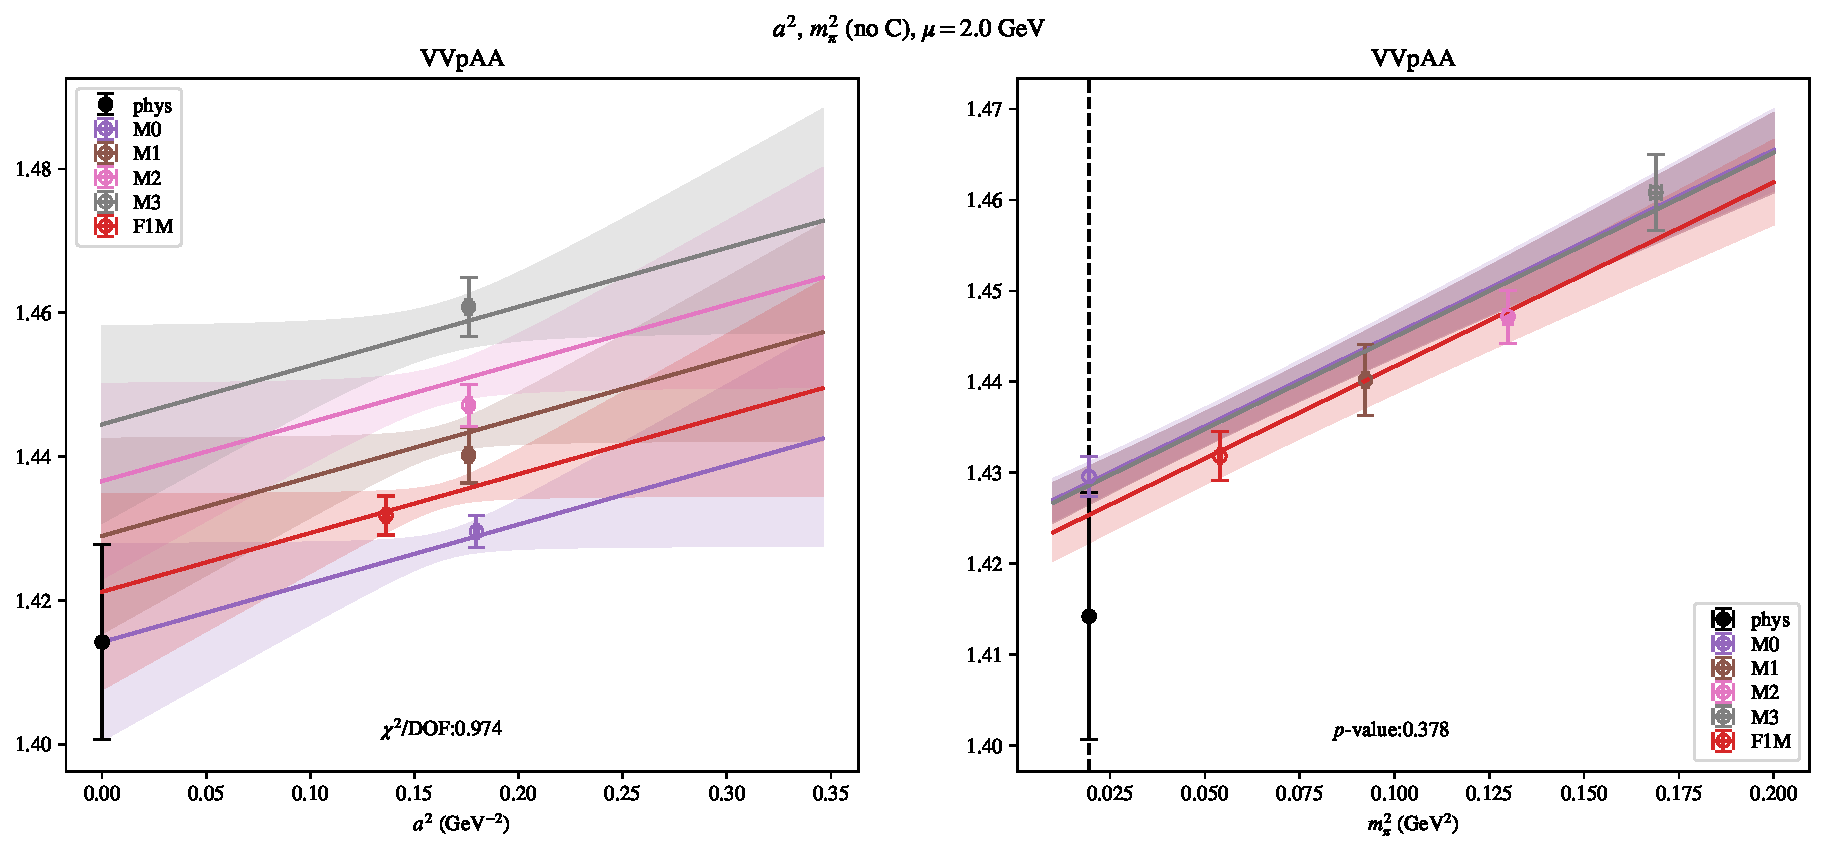
\includepdf[link, pages=-]{VVpAA/NPR/a2m2noC_20.pdf}
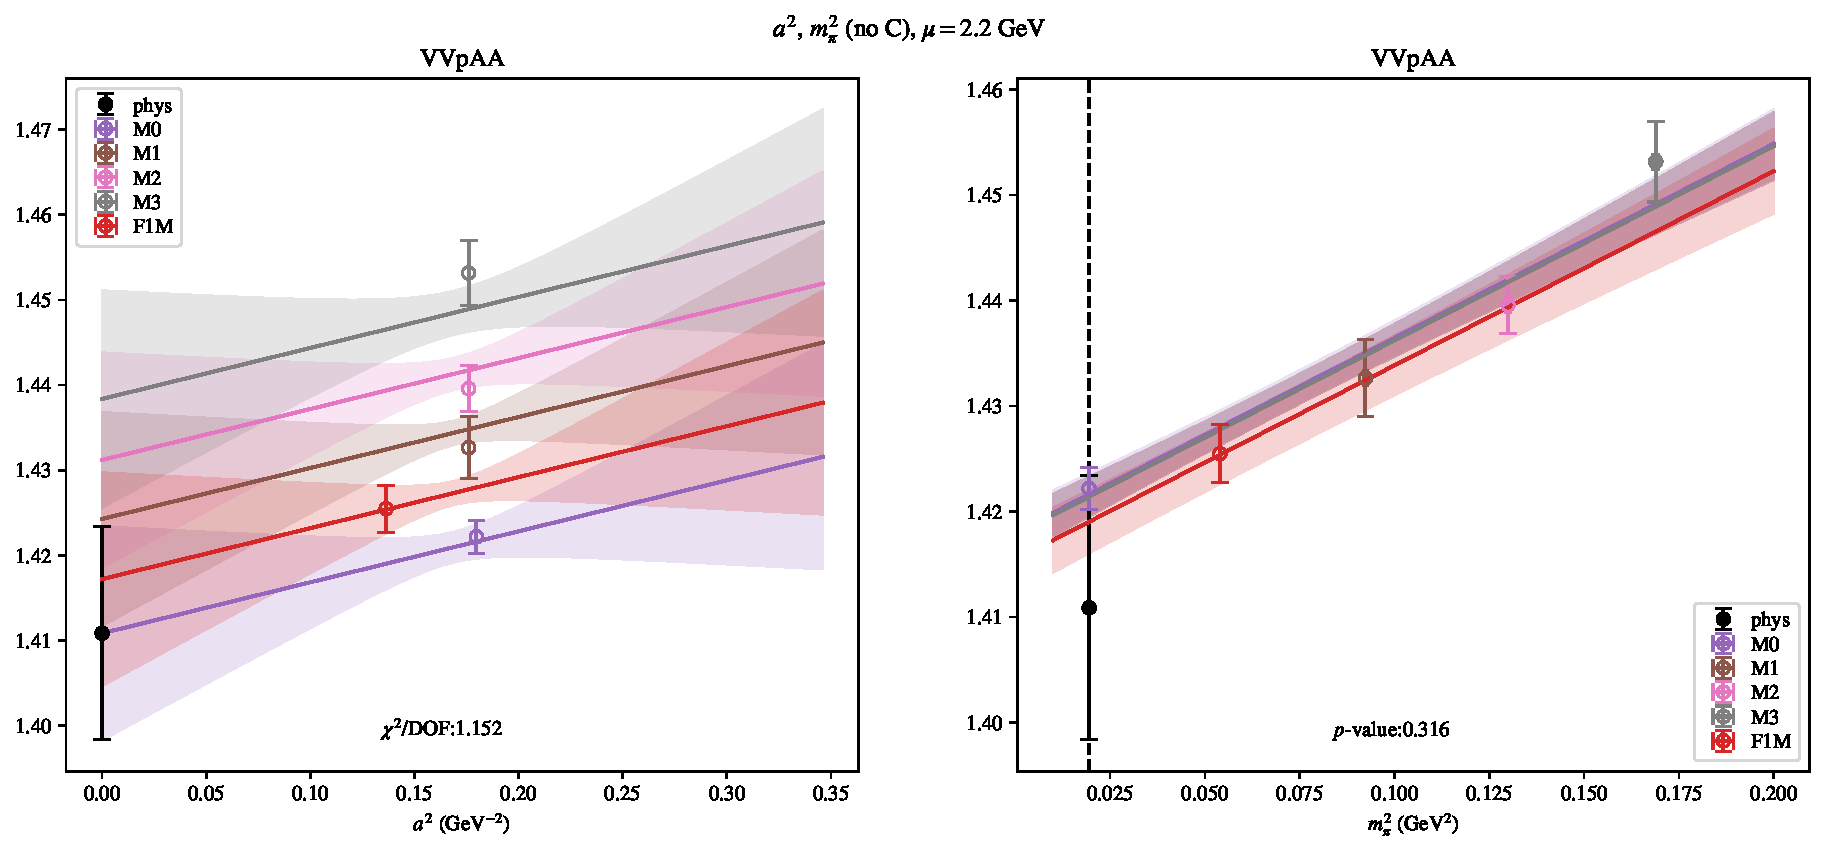
\includepdf[link, pages=-]{VVpAA/NPR/a2m2noC_22.pdf}
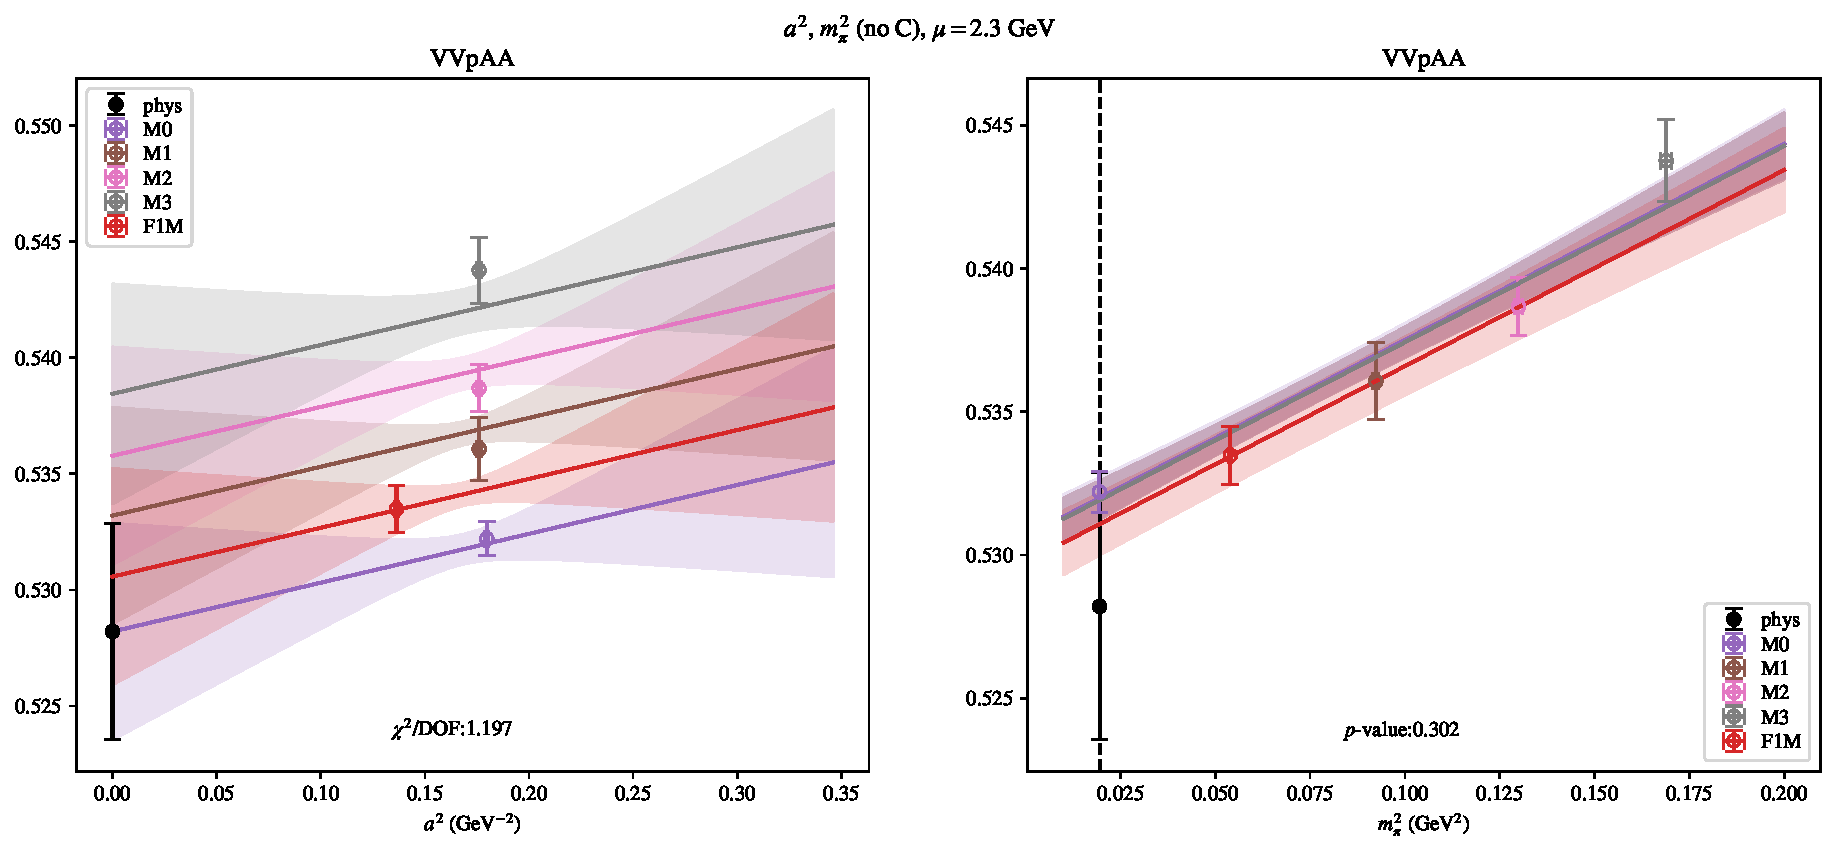
\includepdf[link, pages=-]{VVpAA/NPR/a2m2noC_23.pdf}
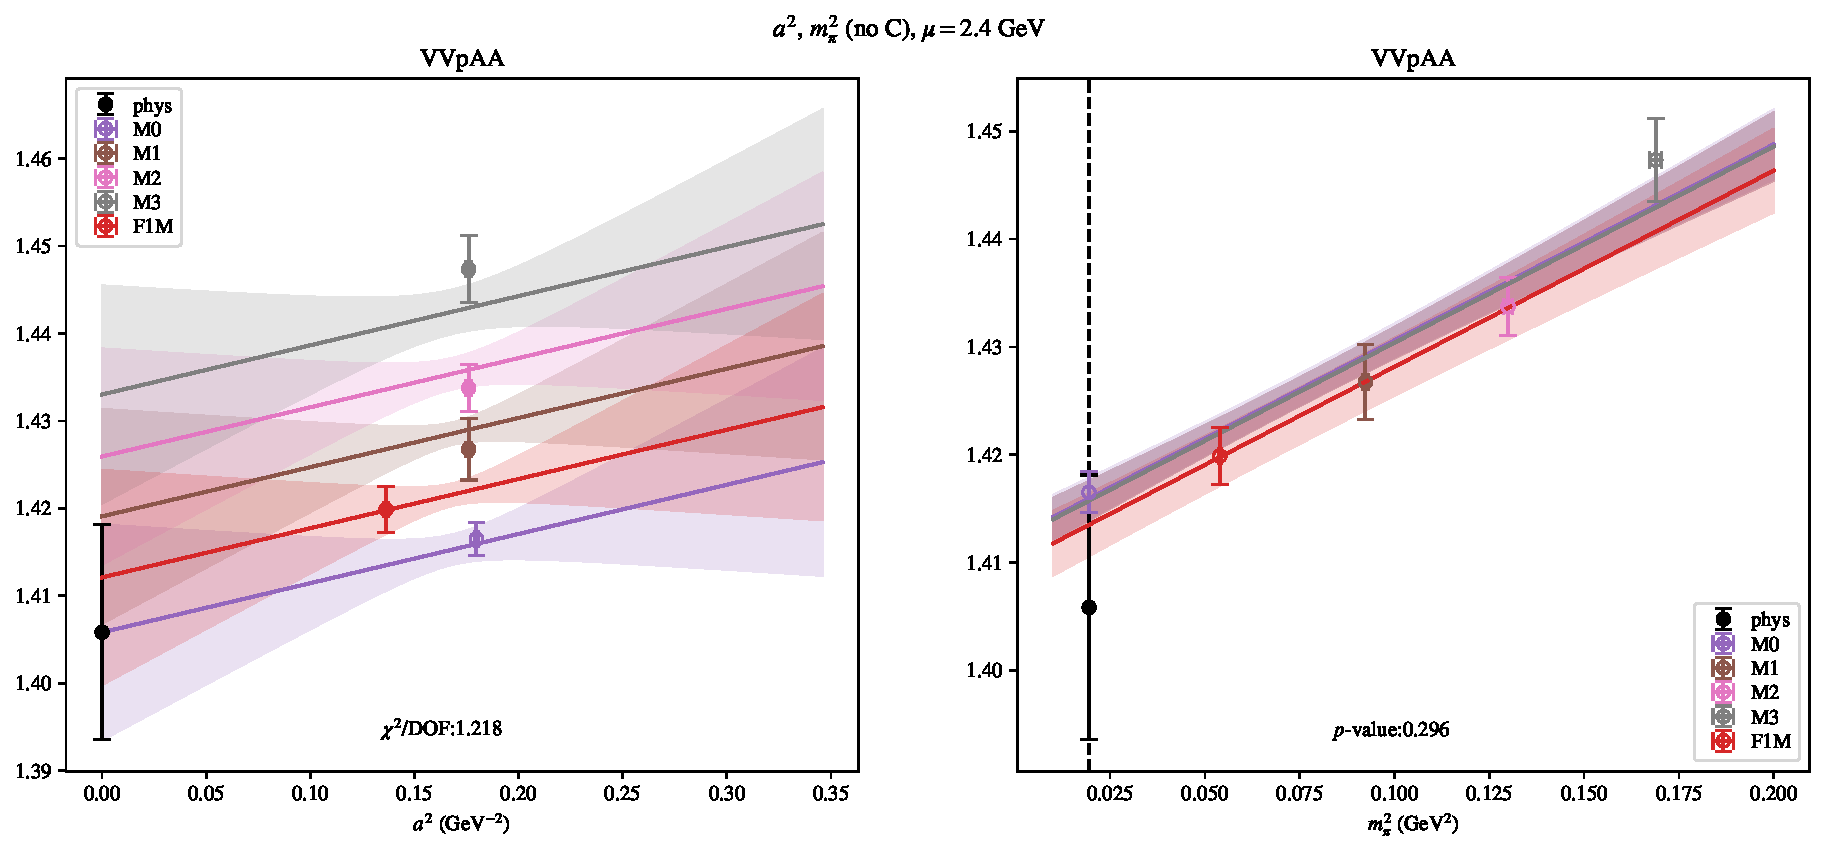
\includepdf[link, pages=-]{VVpAA/NPR/a2m2noC_24.pdf}
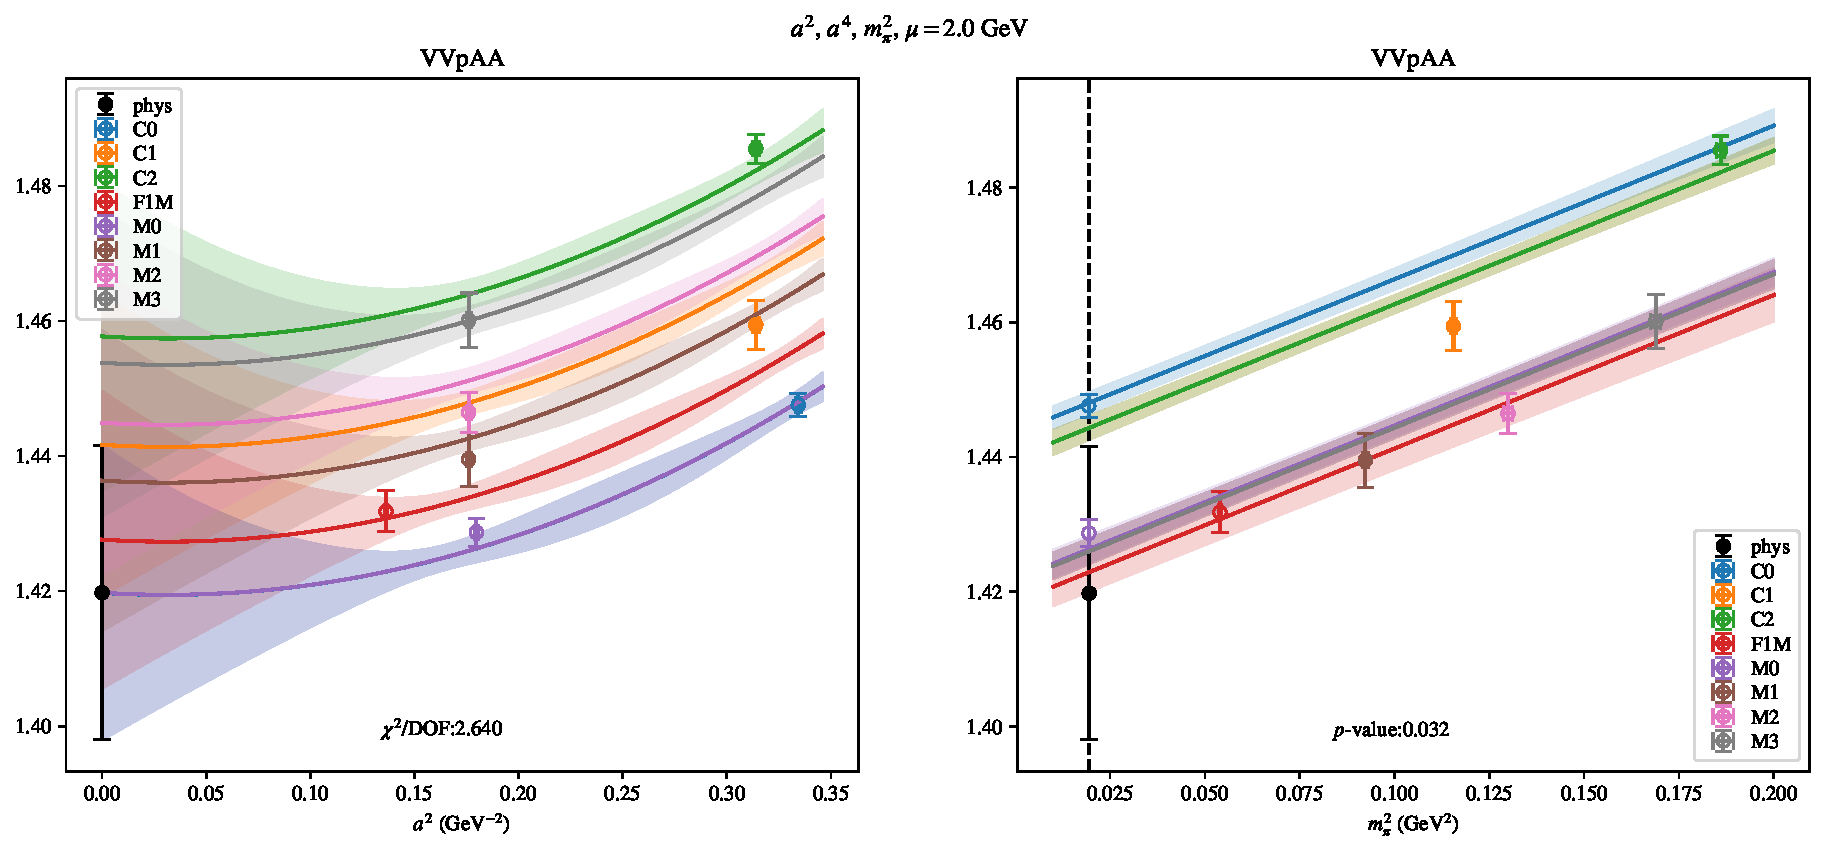
\includepdf[link, pages=-]{VVpAA/NPR/a2a4m2_20.pdf}
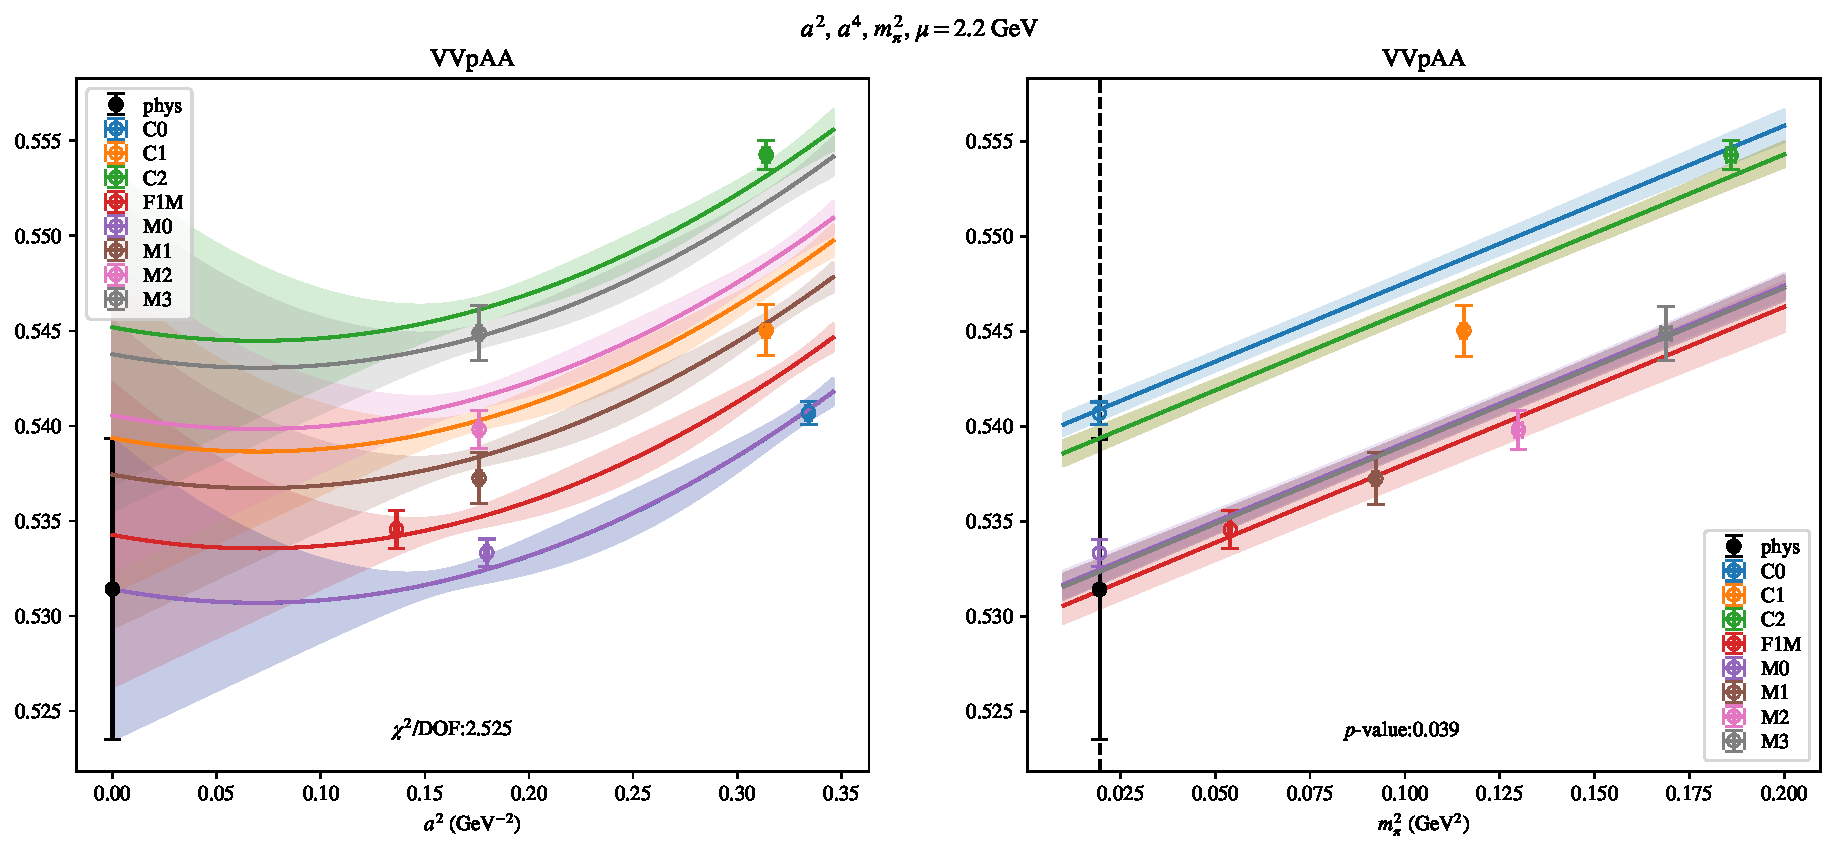
\includepdf[link, pages=-]{VVpAA/NPR/a2a4m2_22.pdf}
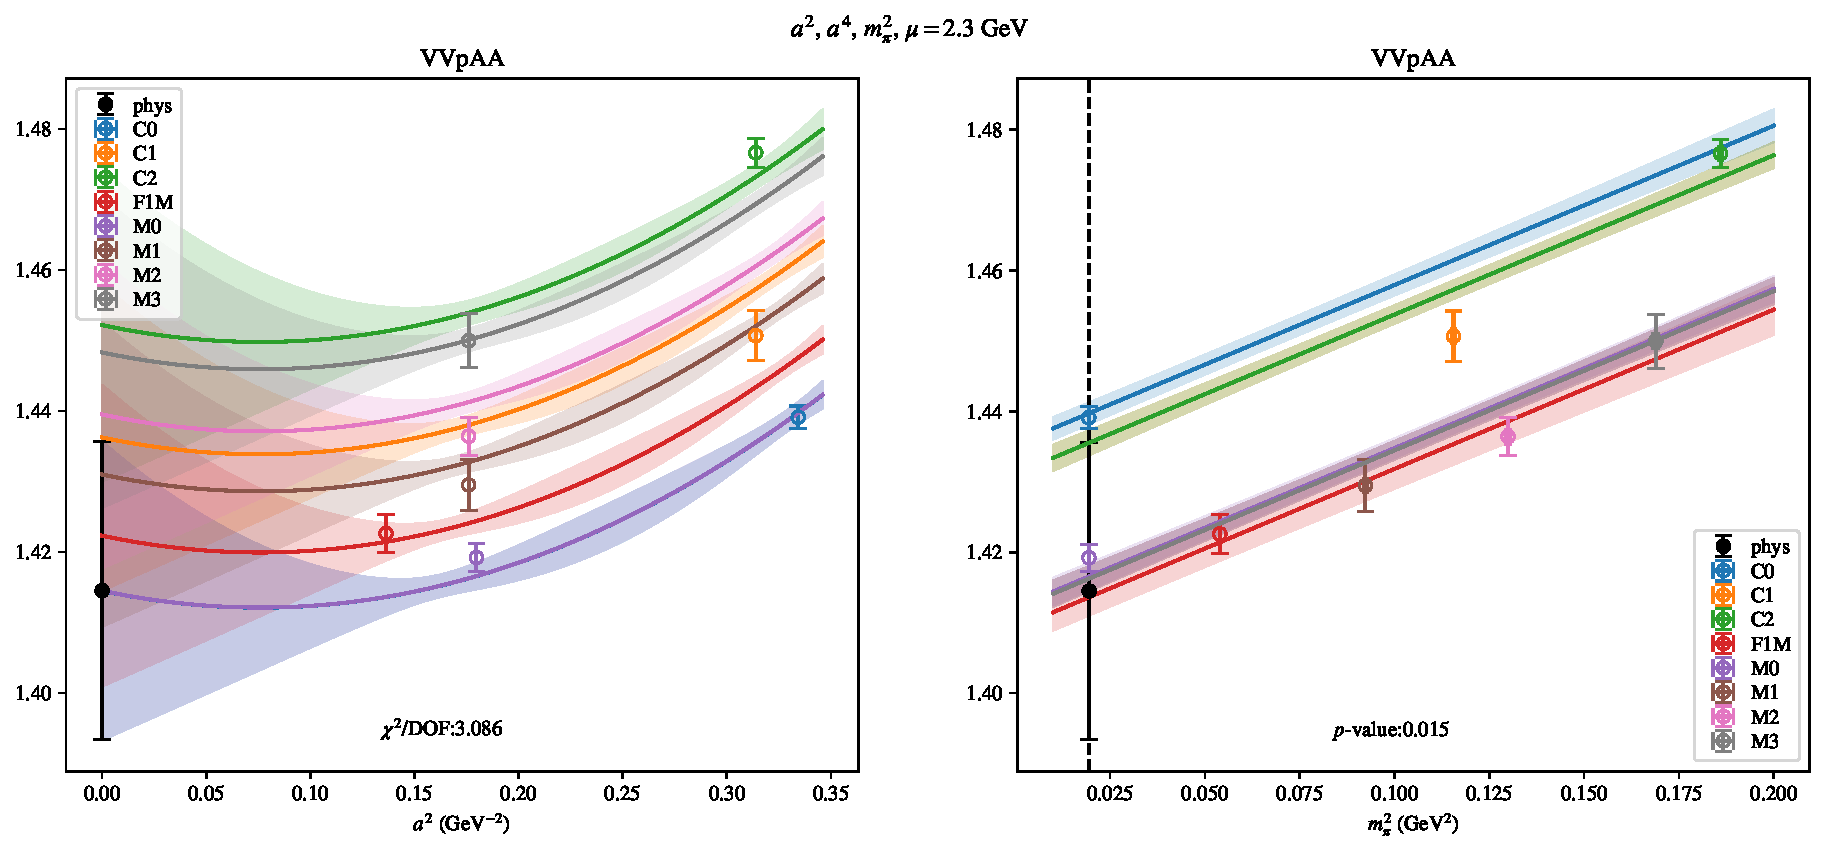
\includepdf[link, pages=-]{VVpAA/NPR/a2a4m2_23.pdf}
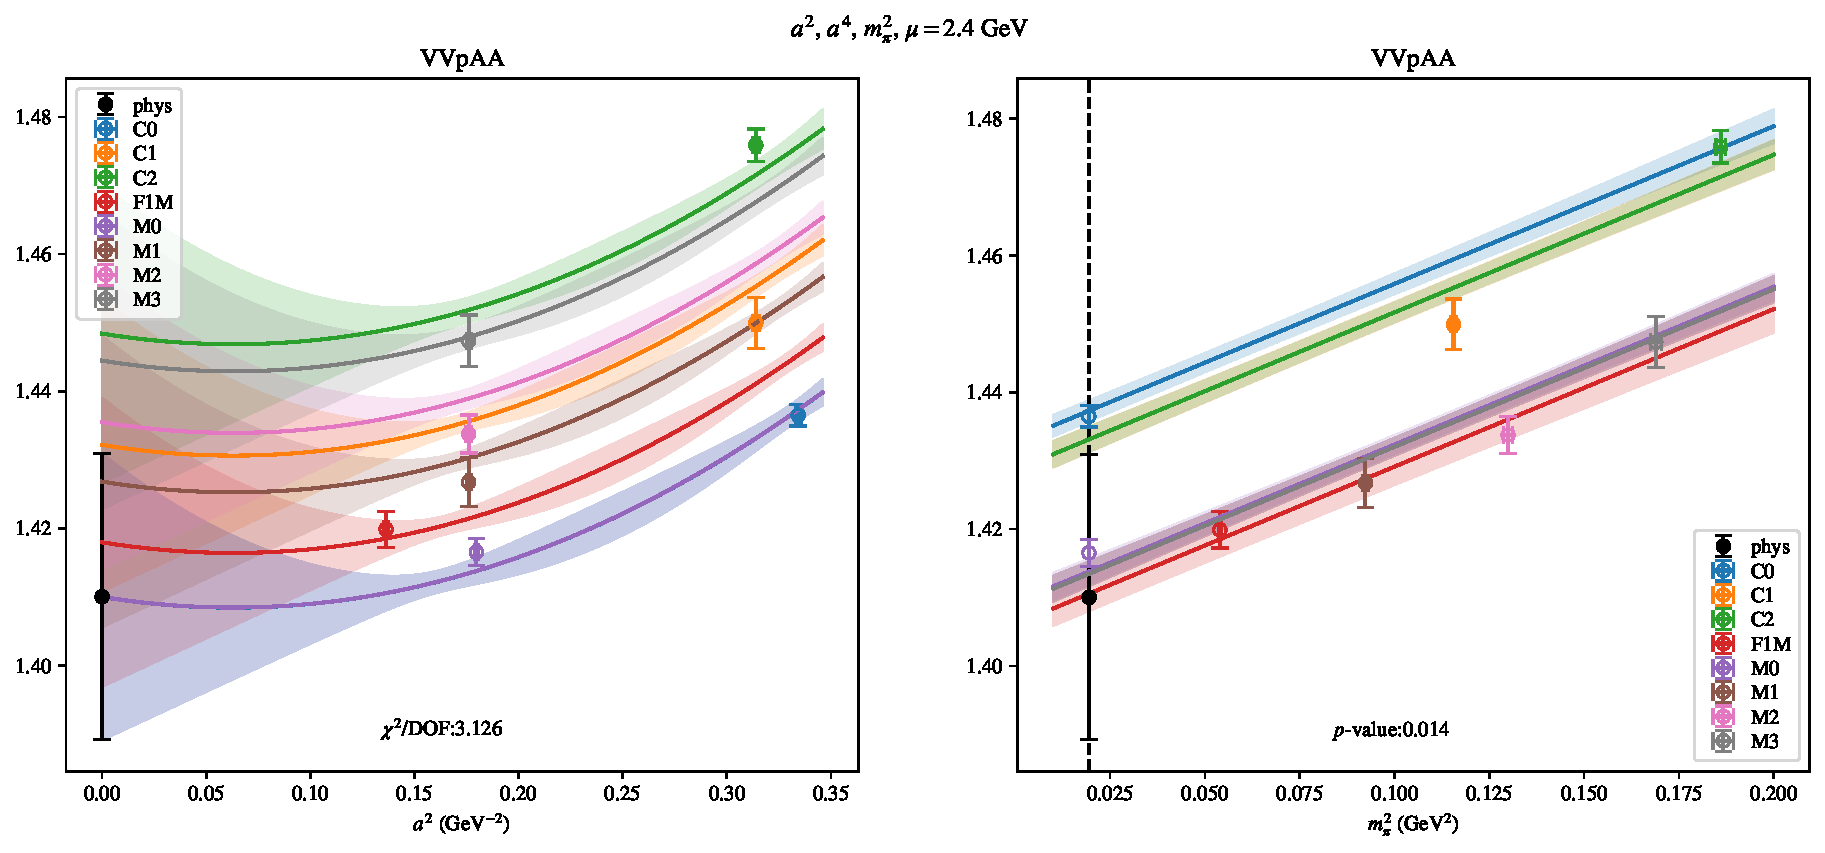
\includepdf[link, pages=-]{VVpAA/NPR/a2a4m2_24.pdf}
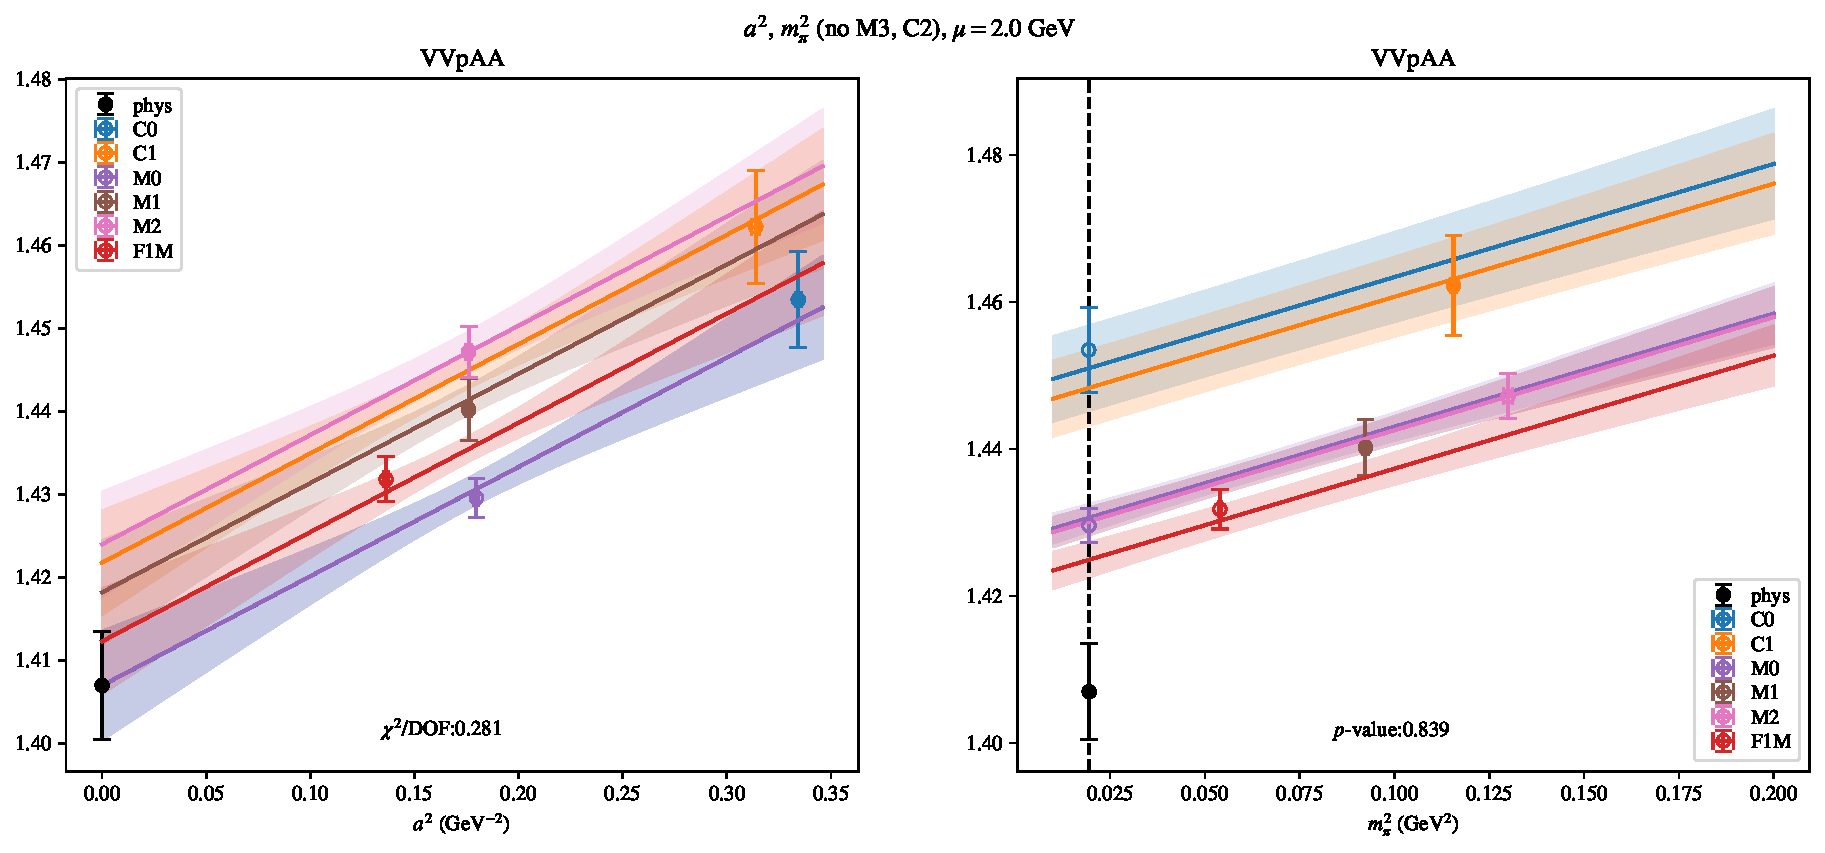
\includepdf[link, pages=-]{VVpAA/NPR/a2m2mcut_20.pdf}
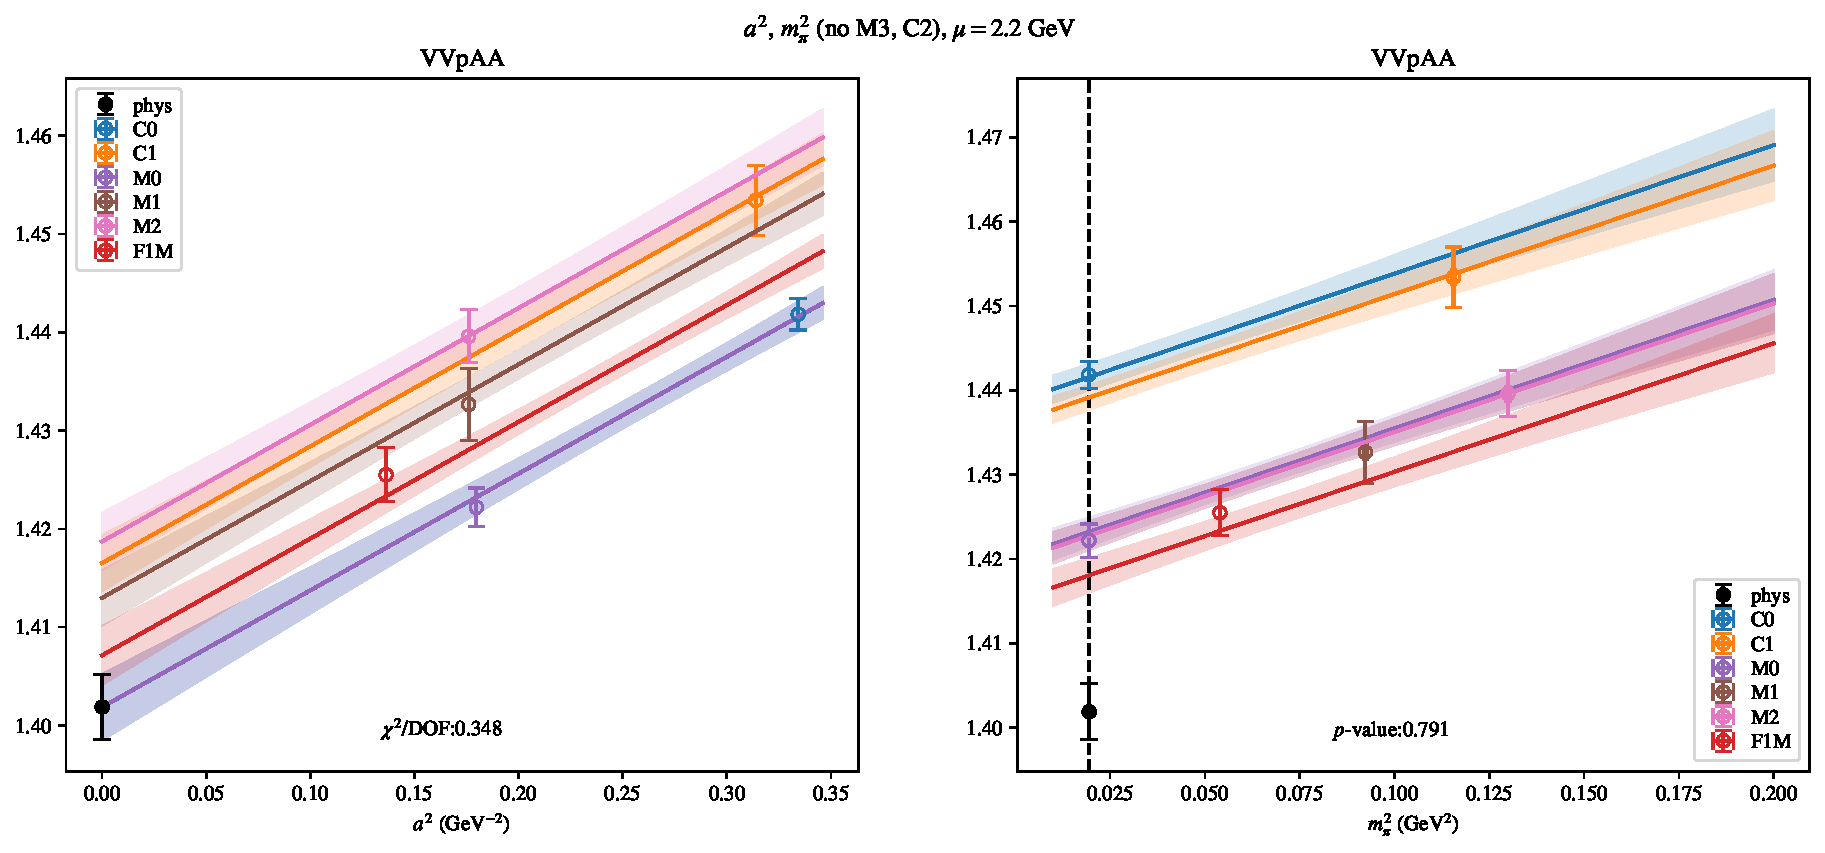
\includepdf[link, pages=-]{VVpAA/NPR/a2m2mcut_22.pdf}
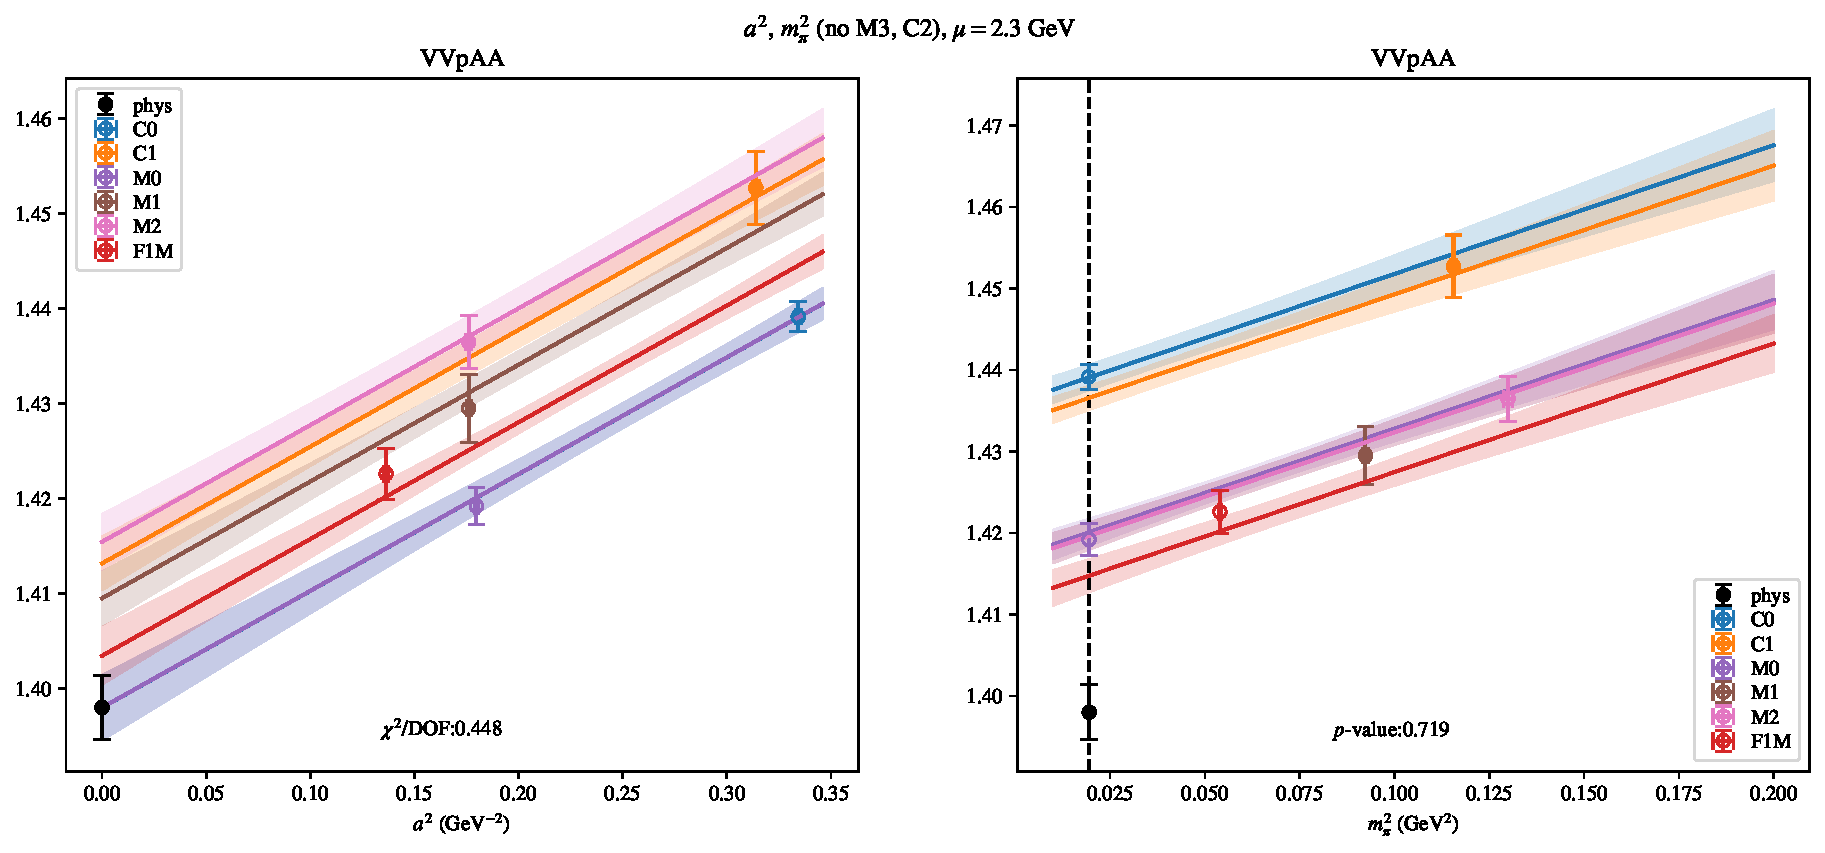
\includepdf[link, pages=-]{VVpAA/NPR/a2m2mcut_23.pdf}
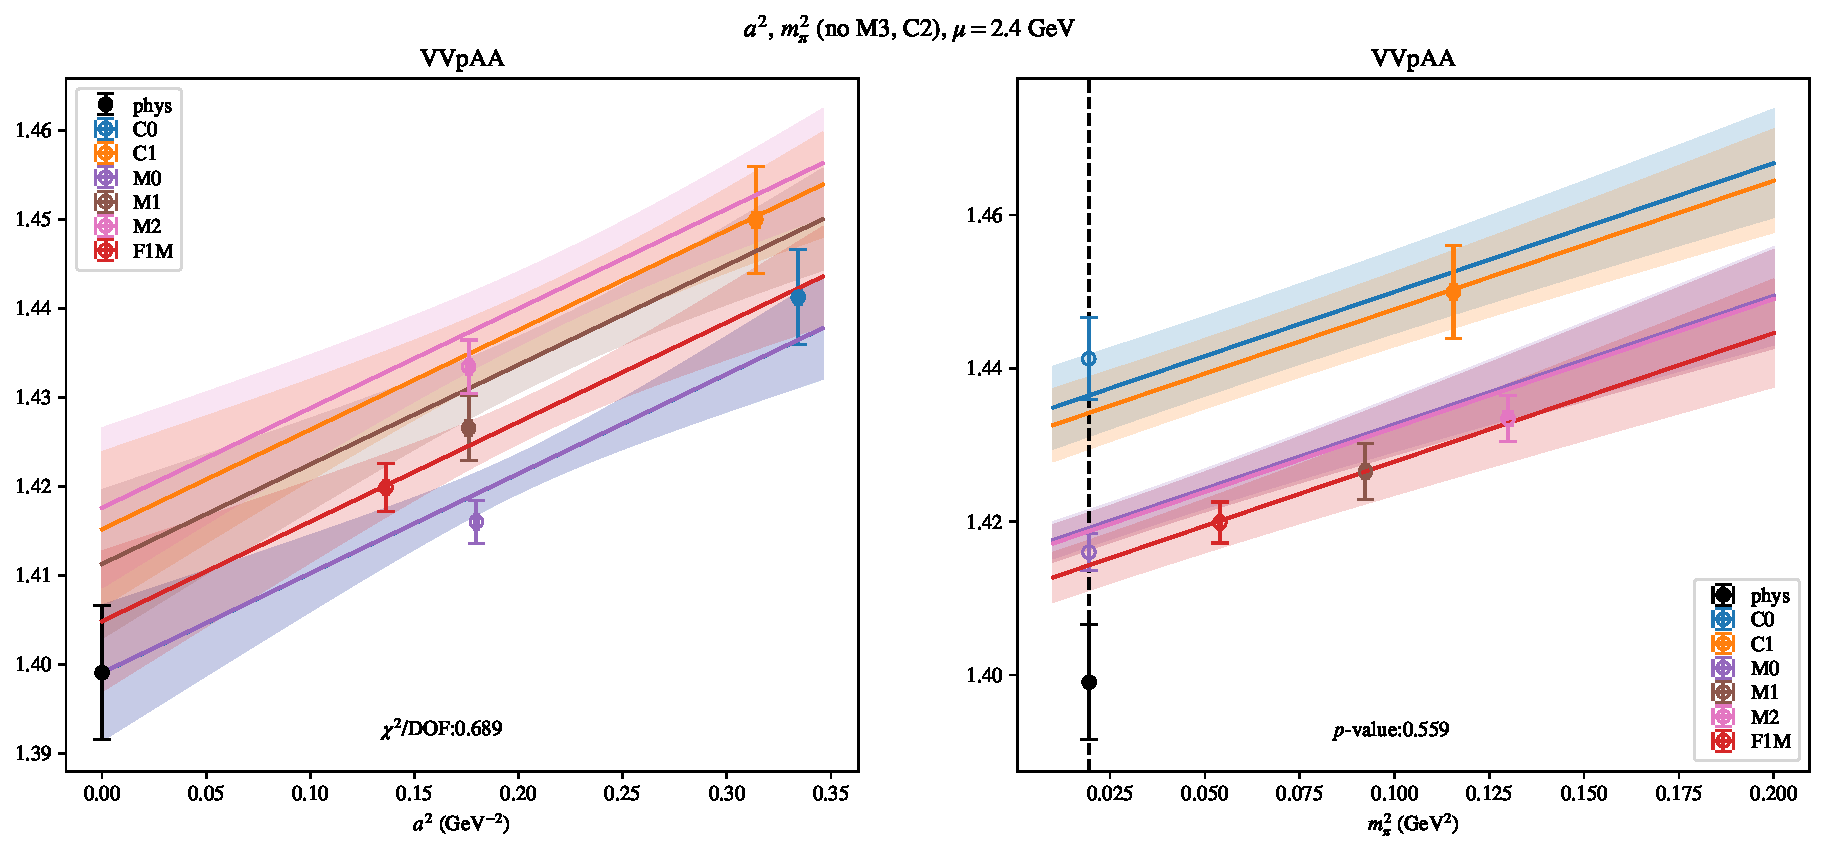
\includepdf[link, pages=-]{VVpAA/NPR/a2m2mcut_24.pdf}
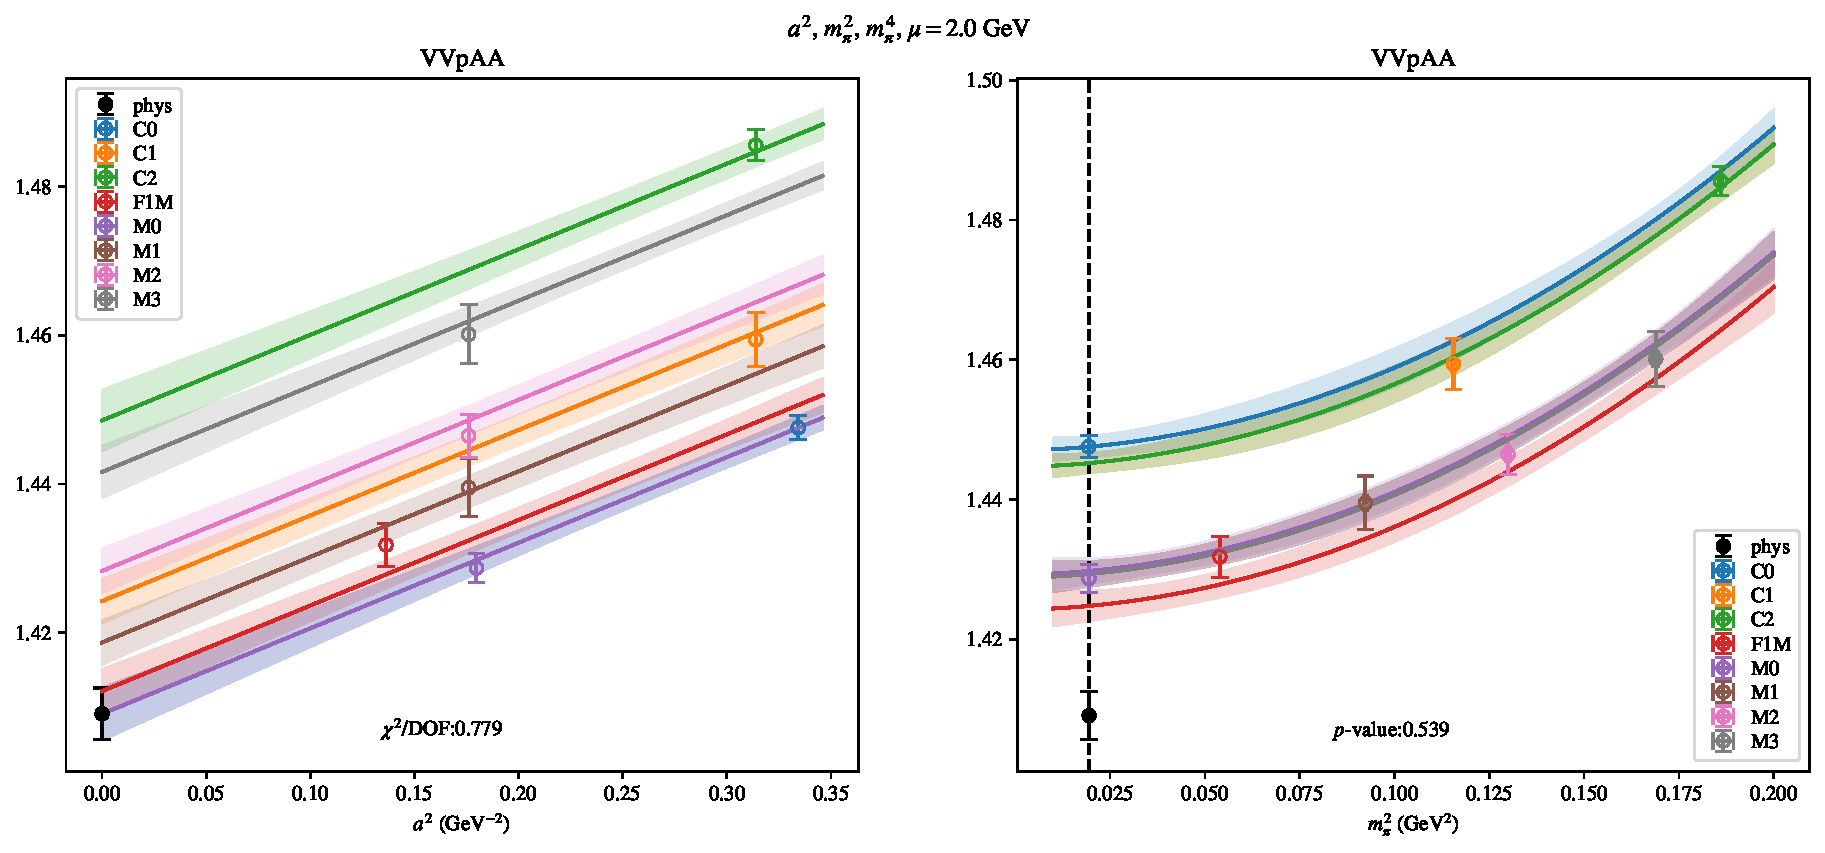
\includepdf[link, pages=-]{VVpAA/NPR/a2m2m4_20.pdf}
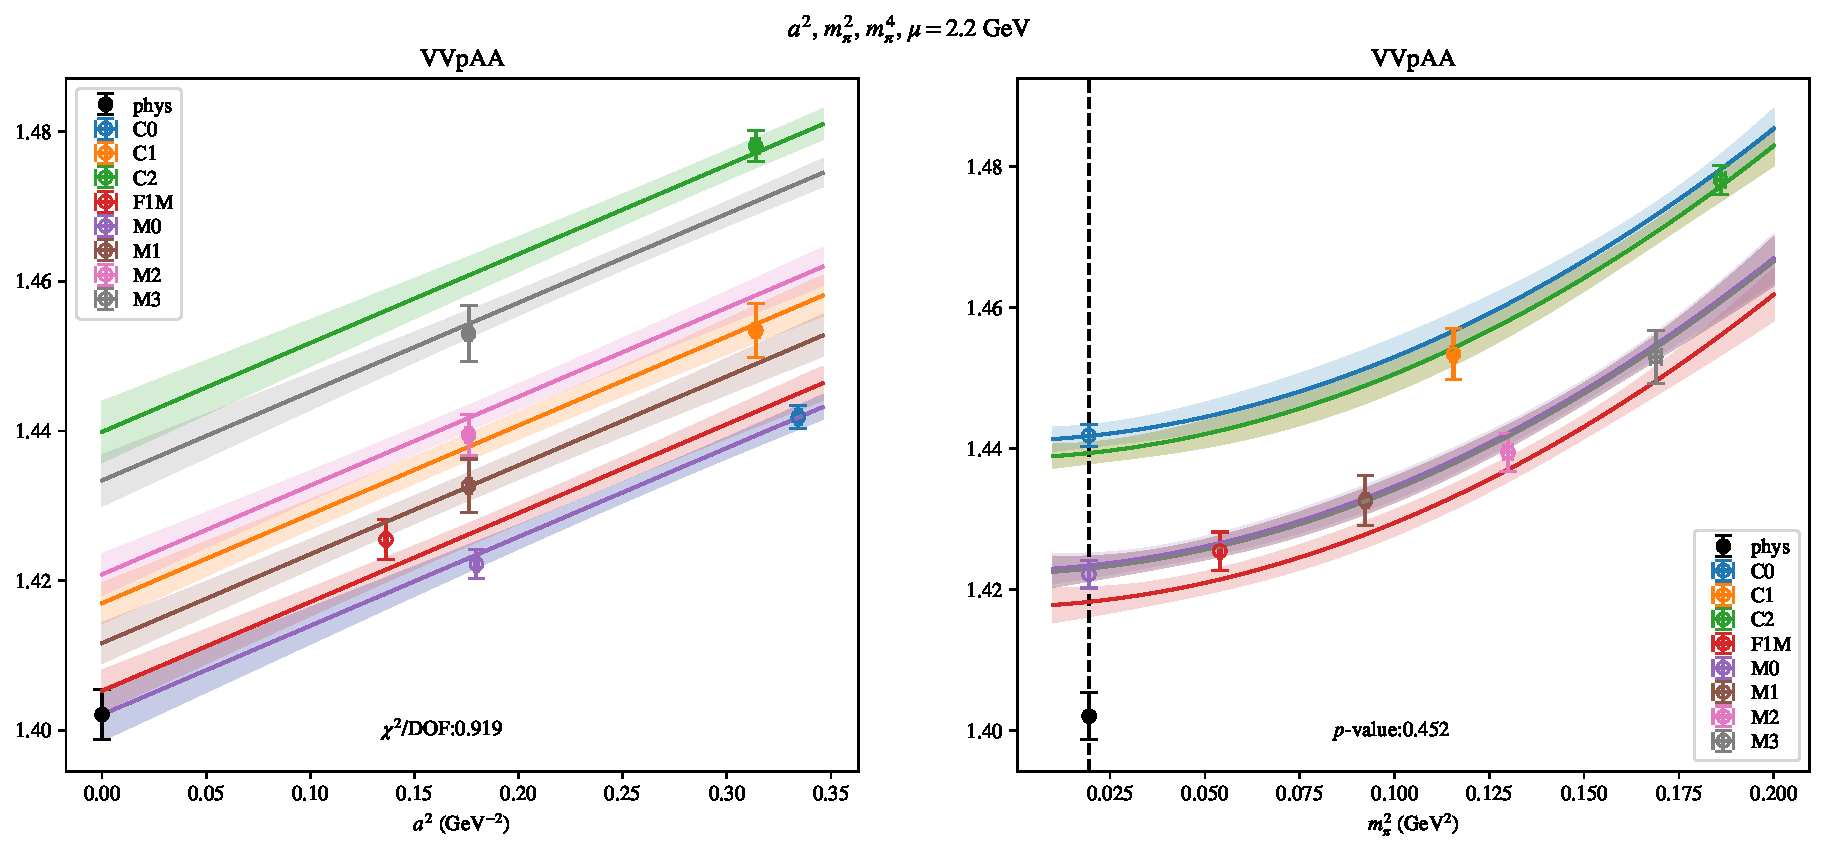
\includepdf[link, pages=-]{VVpAA/NPR/a2m2m4_22.pdf}
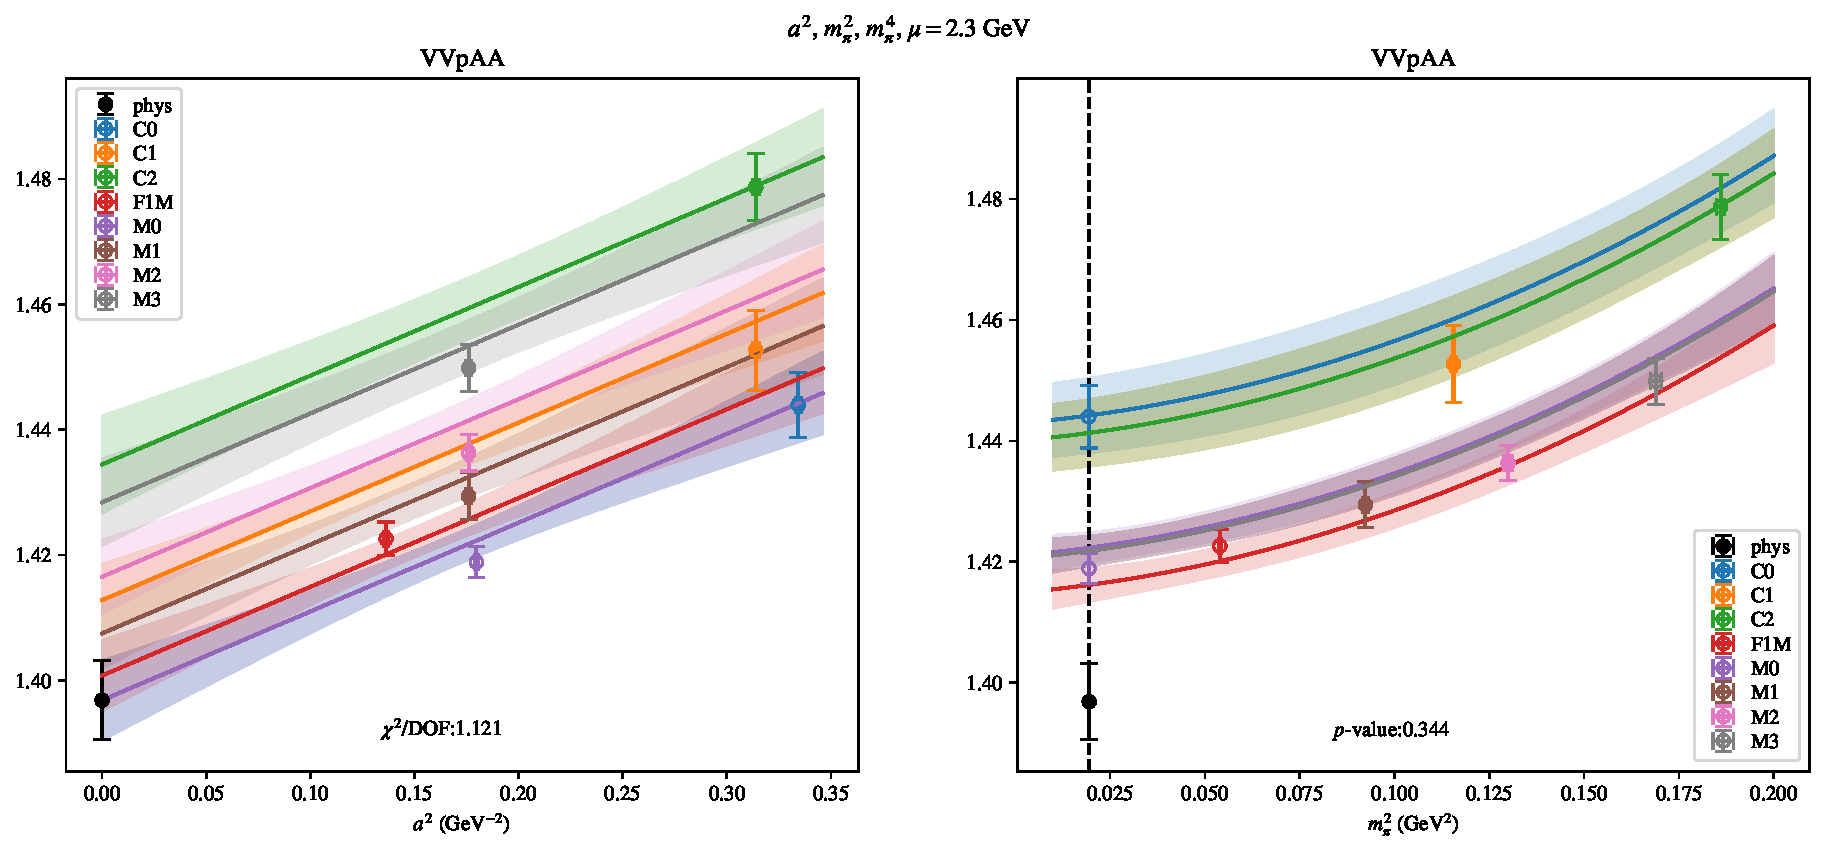
\includepdf[link, pages=-]{VVpAA/NPR/a2m2m4_23.pdf}
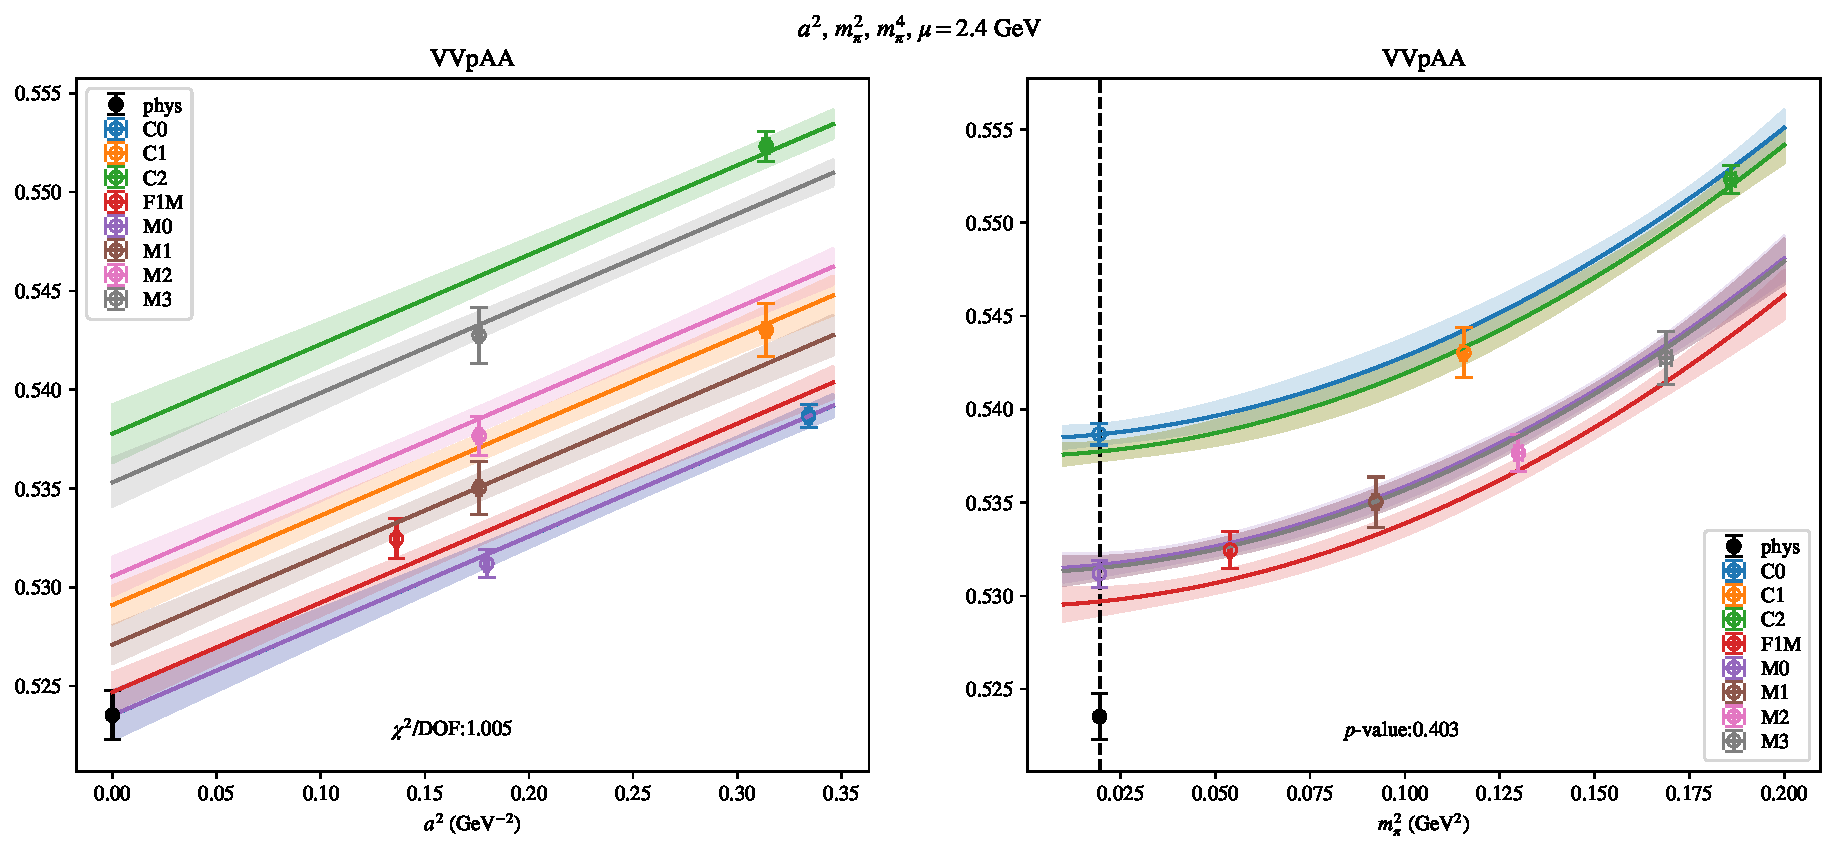
\includepdf[link, pages=-]{VVpAA/NPR/a2m2m4_24.pdf}
\clearpage
\section{$B_2$}
\begin{table}[h!]
\begin{center}
\begin{tabular}{|c|c|c|c|c|c|}
\hline
$\mu$ (GeV) & $a^2$, $m_\pi^2$& $a^2$, $m_\pi^2$ (no C)& $a^2$, $a^4$, $m_\pi^2$& $a^2$, $m_\pi^2$ (no M3, C2)& $a^2$, $m_\pi^2$, $m_\pi^4$\\
\hline
2.0& \hyperlink{VVmAA/NPR/a2m2_20.pdf.1}{\textbf{-1.082(20)}: 0.775 (0.568)} & \hyperlink{VVmAA/NPR/a2m2noC_20.pdf.1}{\textbf{-1.083(85)}: 1.461 (0.232)} & \hyperlink{VVmAA/NPR/a2a4m2_20.pdf.1}{\textbf{-1.08(13)}: 0.917 (0.453)} & \hyperlink{VVmAA/NPR/a2m2mcut_20.pdf.1}{\textbf{-1.082(19)}: 0.593 (0.619)} & \hyperlink{VVmAA/NPR/a2m2m4_20.pdf.1}{\textbf{-1.083(19)}: 0.839 (0.5)}\\
2.2& \hyperlink{VVmAA/NPR/a2m2_22.pdf.1}{\textbf{-1.042(20)}: 0.499 (0.777)} & \hyperlink{VVmAA/NPR/a2m2noC_22.pdf.1}{\textbf{-1.043(83)}: 1.153 (0.316)} & \hyperlink{VVmAA/NPR/a2a4m2_22.pdf.1}{\textbf{-1.04(12)}: 0.611 (0.654)} & \hyperlink{VVmAA/NPR/a2m2mcut_22.pdf.1}{\textbf{-1.042(19)}: 0.421 (0.738)} & \hyperlink{VVmAA/NPR/a2m2m4_22.pdf.1}{\textbf{-1.043(19)}: 0.524 (0.718)}\\
2.3& \hyperlink{VVmAA/NPR/a2m2_23.pdf.1}{\textbf{-1.025(19)}: 0.588 (0.709)} & \hyperlink{VVmAA/NPR/a2m2noC_23.pdf.1}{\textbf{-1.026(81)}: 1.295 (0.274)} & \hyperlink{VVmAA/NPR/a2a4m2_23.pdf.1}{\textbf{-1.03(12)}: 0.713 (0.583)} & \hyperlink{VVmAA/NPR/a2m2mcut_23.pdf.1}{\textbf{-1.025(18)}: 0.488 (0.691)} & \hyperlink{VVmAA/NPR/a2m2m4_23.pdf.1}{\textbf{-1.026(18)}: 0.623 (0.646)}\\
2.4& \hyperlink{VVmAA/NPR/a2m2_24.pdf.1}{\textbf{-1.012(19)}: 0.829 (0.529)} & \hyperlink{VVmAA/NPR/a2m2noC_24.pdf.1}{\textbf{-1.008(79)}: 1.935 (0.144)} & \hyperlink{VVmAA/NPR/a2a4m2_24.pdf.1}{\textbf{-1.00(12)}: 1.026 (0.392)} & \hyperlink{VVmAA/NPR/a2m2mcut_24.pdf.1}{\textbf{-1.012(18)}: 0.736 (0.53)} & \hyperlink{VVmAA/NPR/a2m2m4_24.pdf.1}{\textbf{-1.012(18)}: 0.765 (0.548)}\\
\hline
\end{tabular}
\caption{Physical point value from chiral and continuum extrapolation at renormalisation scale $\mu$. Entries are \textbf{value(error)}: $\chi^2/\text{DOF}$ ($p$-value).}
\end{center}
\end{table}
\begin{table}[h!]
\begin{center}
\begin{tabular}{|c c|c|c|c|c|c|}
\hline
$\mu$ (GeV) &  & $a^2$, $m_\pi^2$& $a^2$, $m_\pi^2$ (no C)& $a^2$, $a^4$, $m_\pi^2$& $a^2$, $m_\pi^2$ (no M3, C2)& $a^2$, $m_\pi^2$, $m_\pi^4$\\
\hline
\multirow{2}{0.5in}{2.0} & $\alpha$ & -0.400(43)& -0.40(42)& -0.4(10)& -0.398(47)& -0.401(46)\\
 & $\beta$ & 0.00174(15)& 0.00194(25)& 0.00176(15)& 0.00160(25)& 0.00117(65)\\
\hline
\multirow{2}{0.5in}{2.2} & $\alpha$ & -0.393(43)& -0.39(41)& -0.4(10)& -0.392(45)& -0.394(45)\\
 & $\beta$ & 0.00139(13)& 0.00147(23)& 0.00139(13)& 0.00125(25)& 0.00091(68)\\
\hline
\multirow{2}{0.5in}{2.3} & $\alpha$ & -0.388(43)& -0.39(41)& -0.4(10)& -0.387(44)& -0.390(44)\\
 & $\beta$ & 0.00128(13)& 0.00139(22)& 0.00129(13)& 0.00115(24)& 0.00080(67)\\
\hline
\multirow{2}{0.5in}{2.4} & $\alpha$ & -0.389(43)& -0.37(41)& -0.3(10)& -0.388(45)& -0.391(45)\\
 & $\beta$ & 0.00125(11)& 0.00132(20)& 0.00124(12)& 0.00108(21)& 0.00053(62)\\
\hline
\end{tabular}
\caption{Fit values of coefficients in $B = B_{phys} + \mathbf{\alpha} a^2 + \mathbf{\beta}\left(\frac{m_\pi^2}{f_\pi^2}-\frac{m_{\pi,PDG}^2}{f_\pi^2}\right) + \ldots$.}
\end{center}
\end{table}
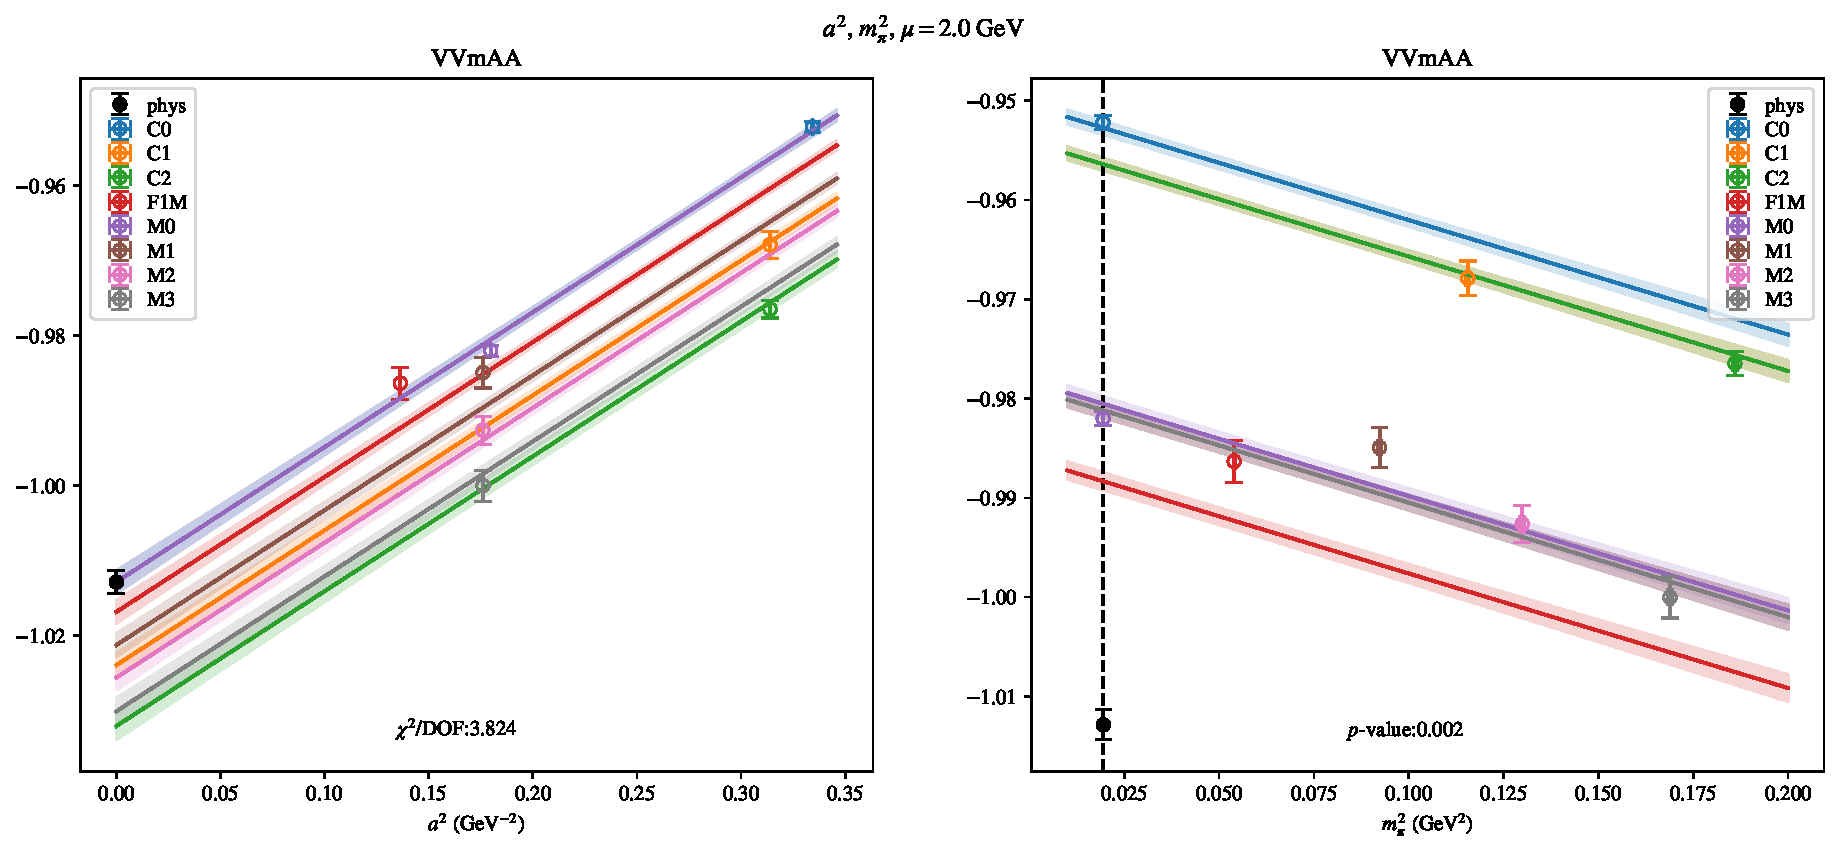
\includepdf[link, pages=-]{VVmAA/NPR/a2m2_20.pdf}
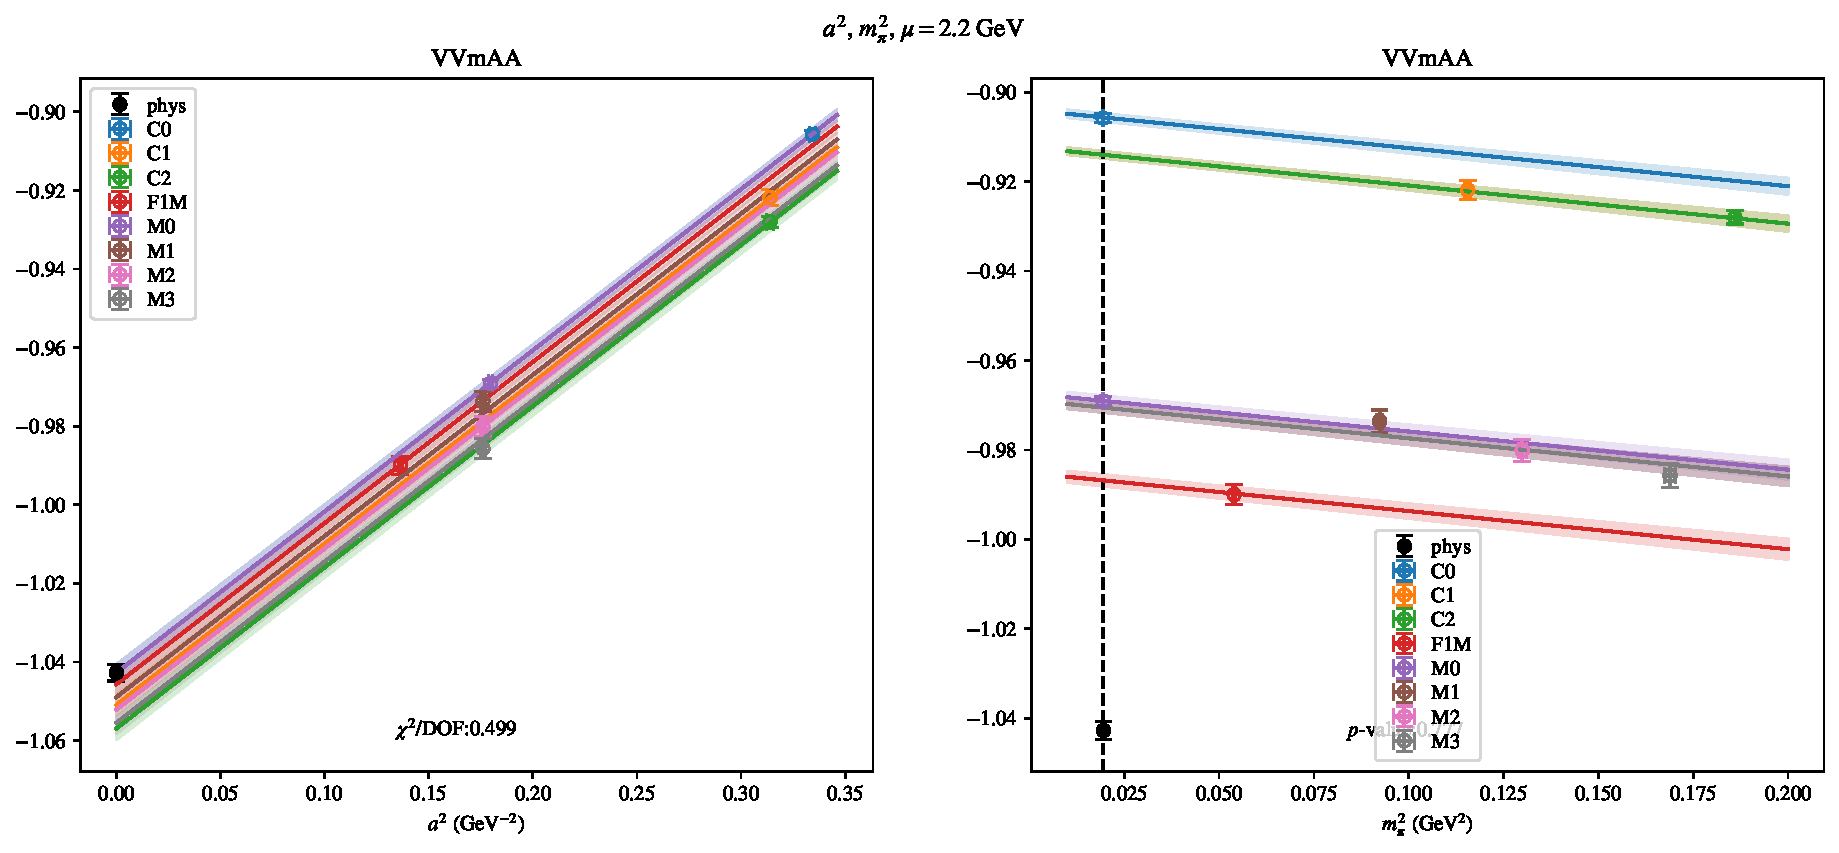
\includepdf[link, pages=-]{VVmAA/NPR/a2m2_22.pdf}
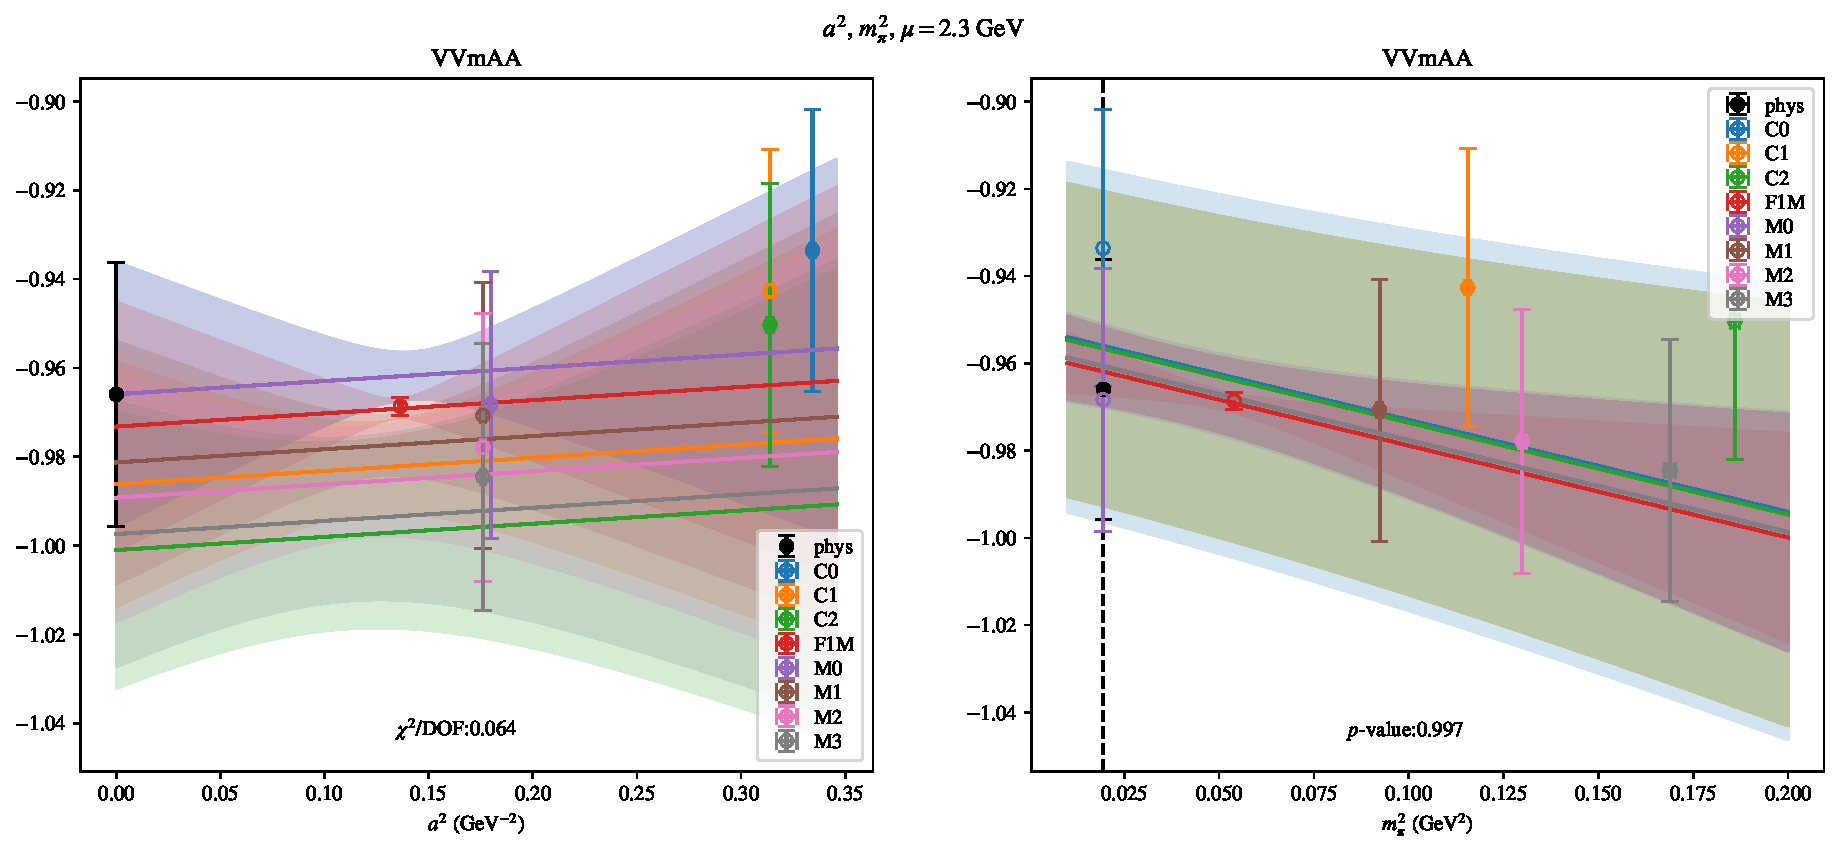
\includepdf[link, pages=-]{VVmAA/NPR/a2m2_23.pdf}
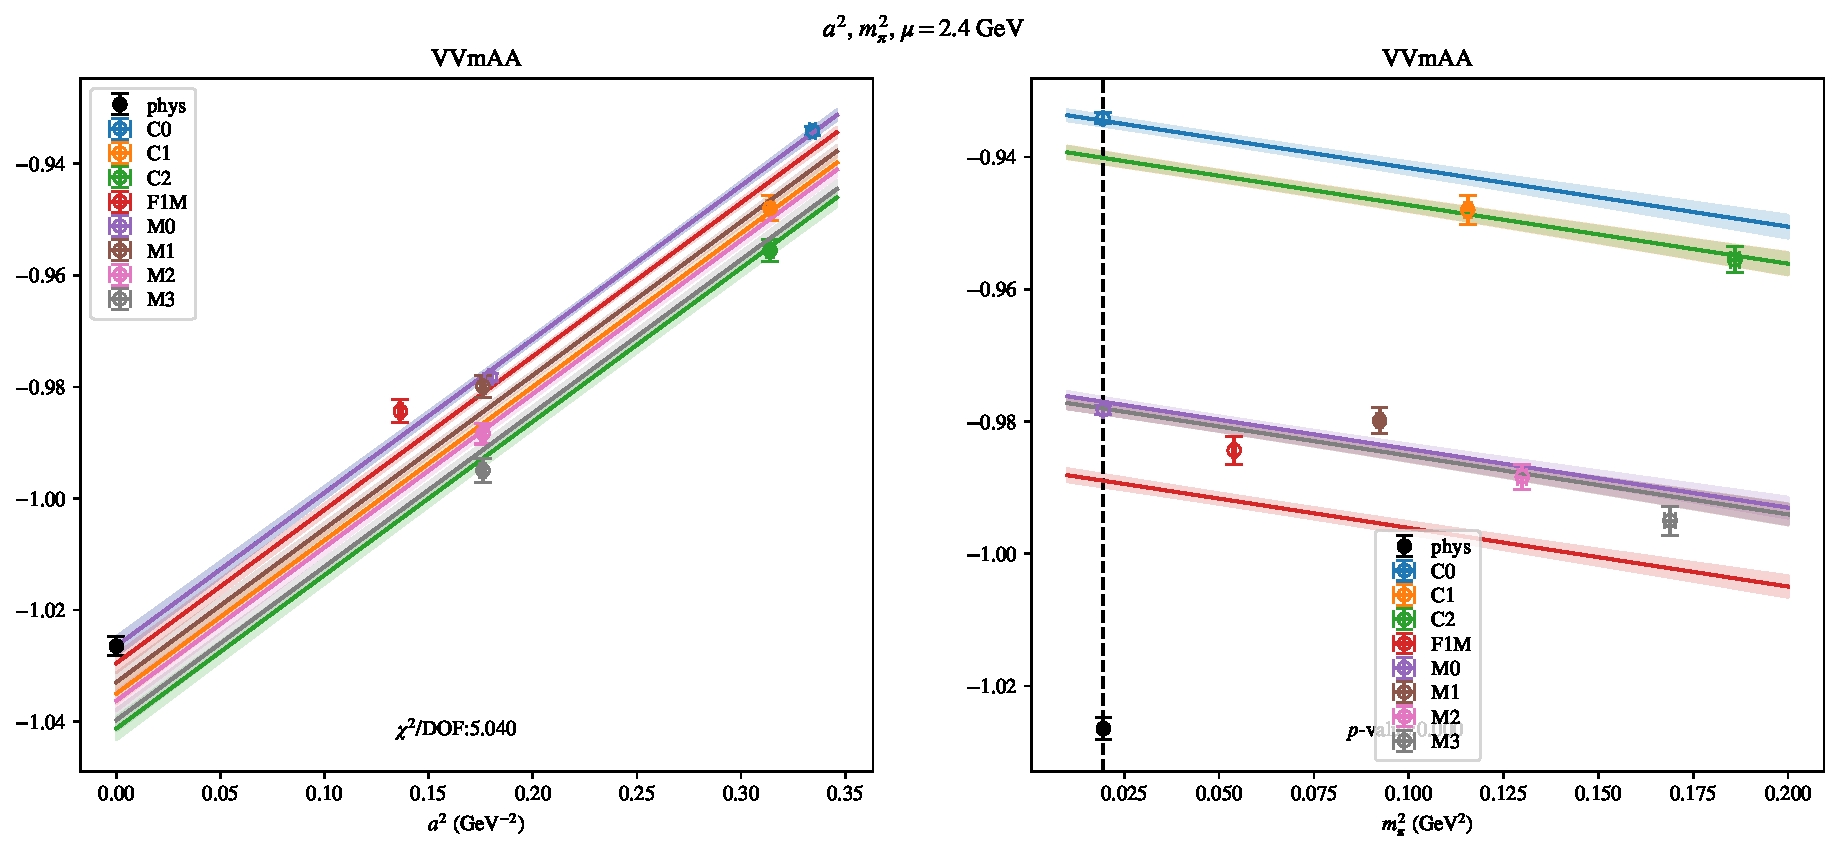
\includepdf[link, pages=-]{VVmAA/NPR/a2m2_24.pdf}
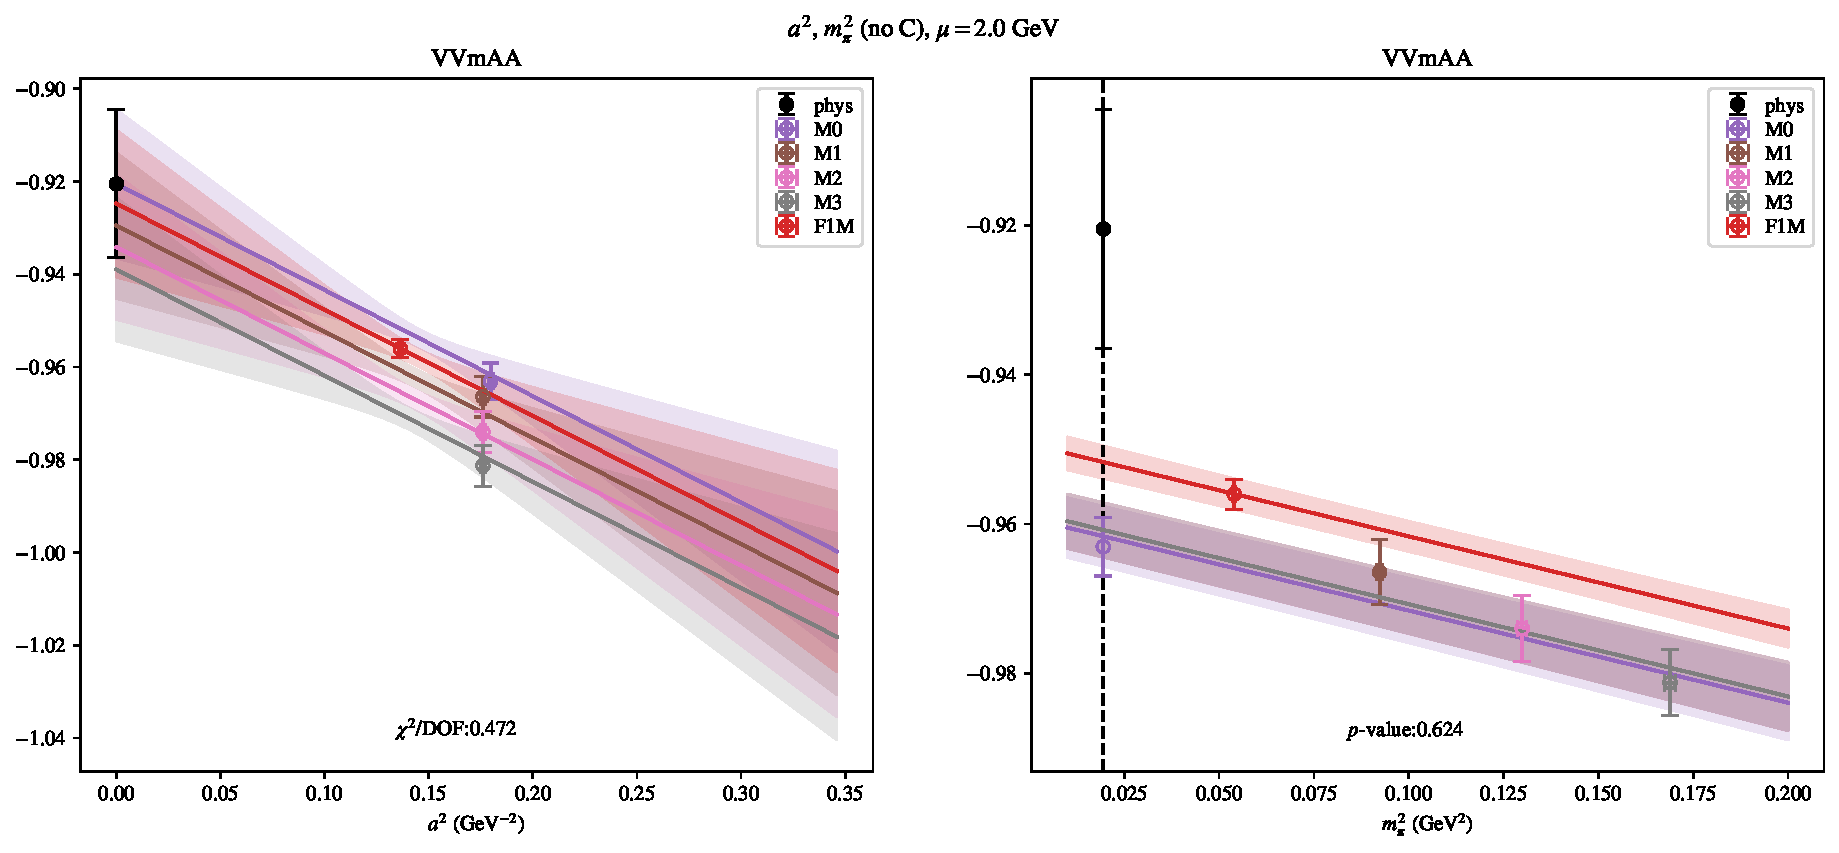
\includepdf[link, pages=-]{VVmAA/NPR/a2m2noC_20.pdf}
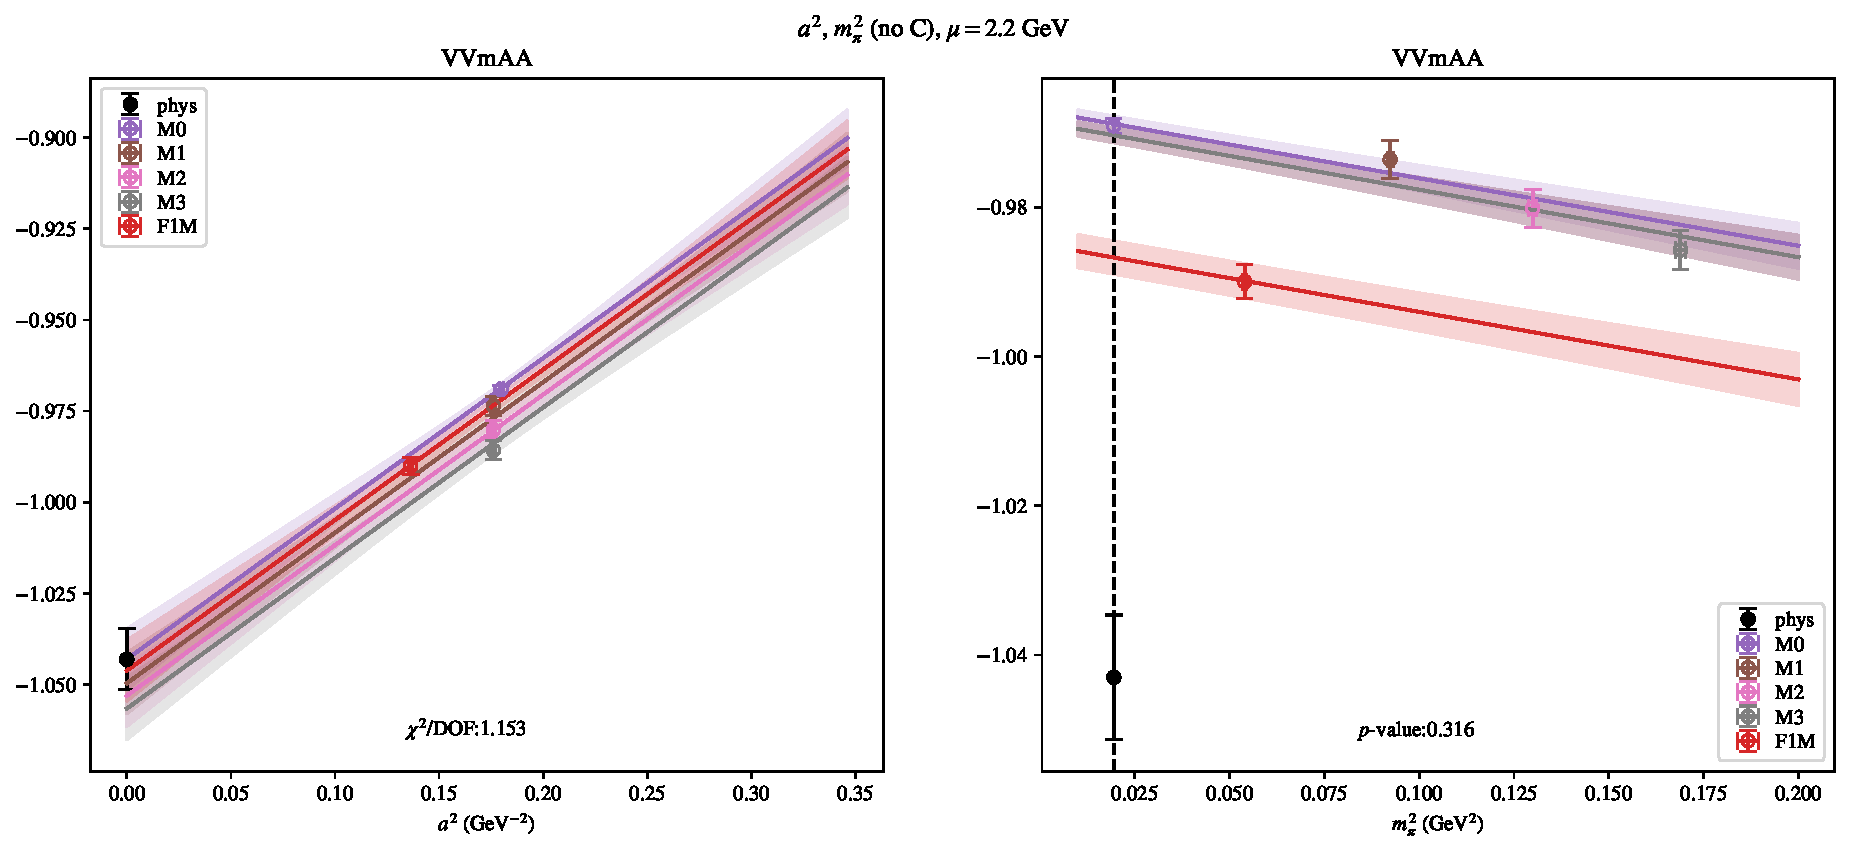
\includepdf[link, pages=-]{VVmAA/NPR/a2m2noC_22.pdf}
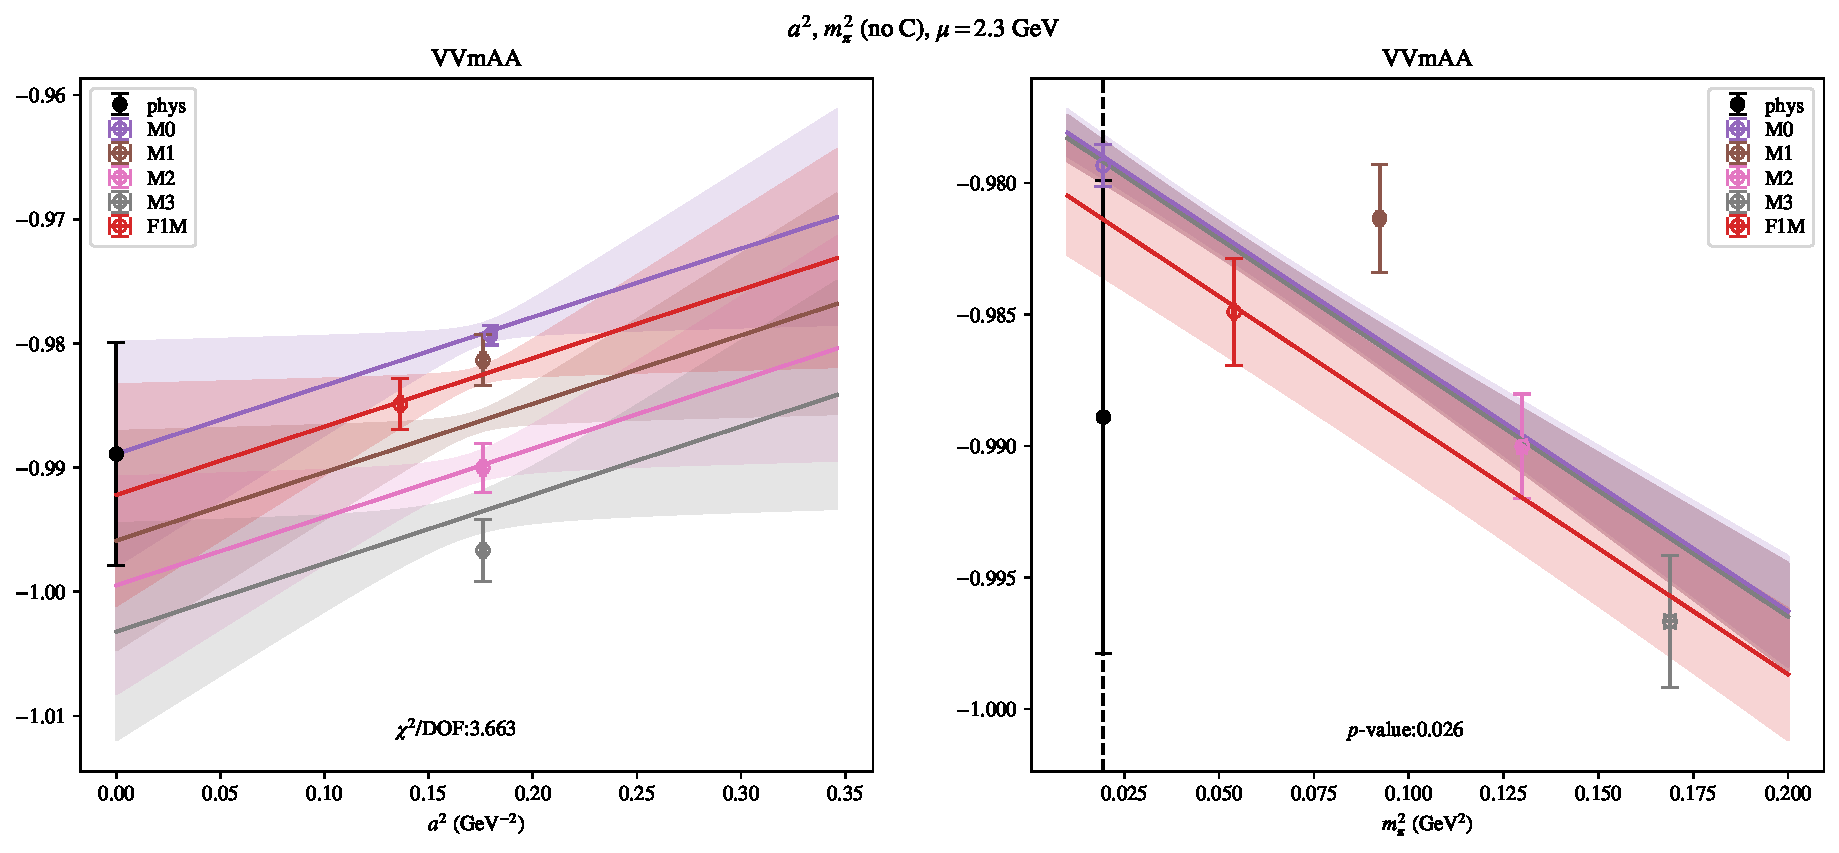
\includepdf[link, pages=-]{VVmAA/NPR/a2m2noC_23.pdf}
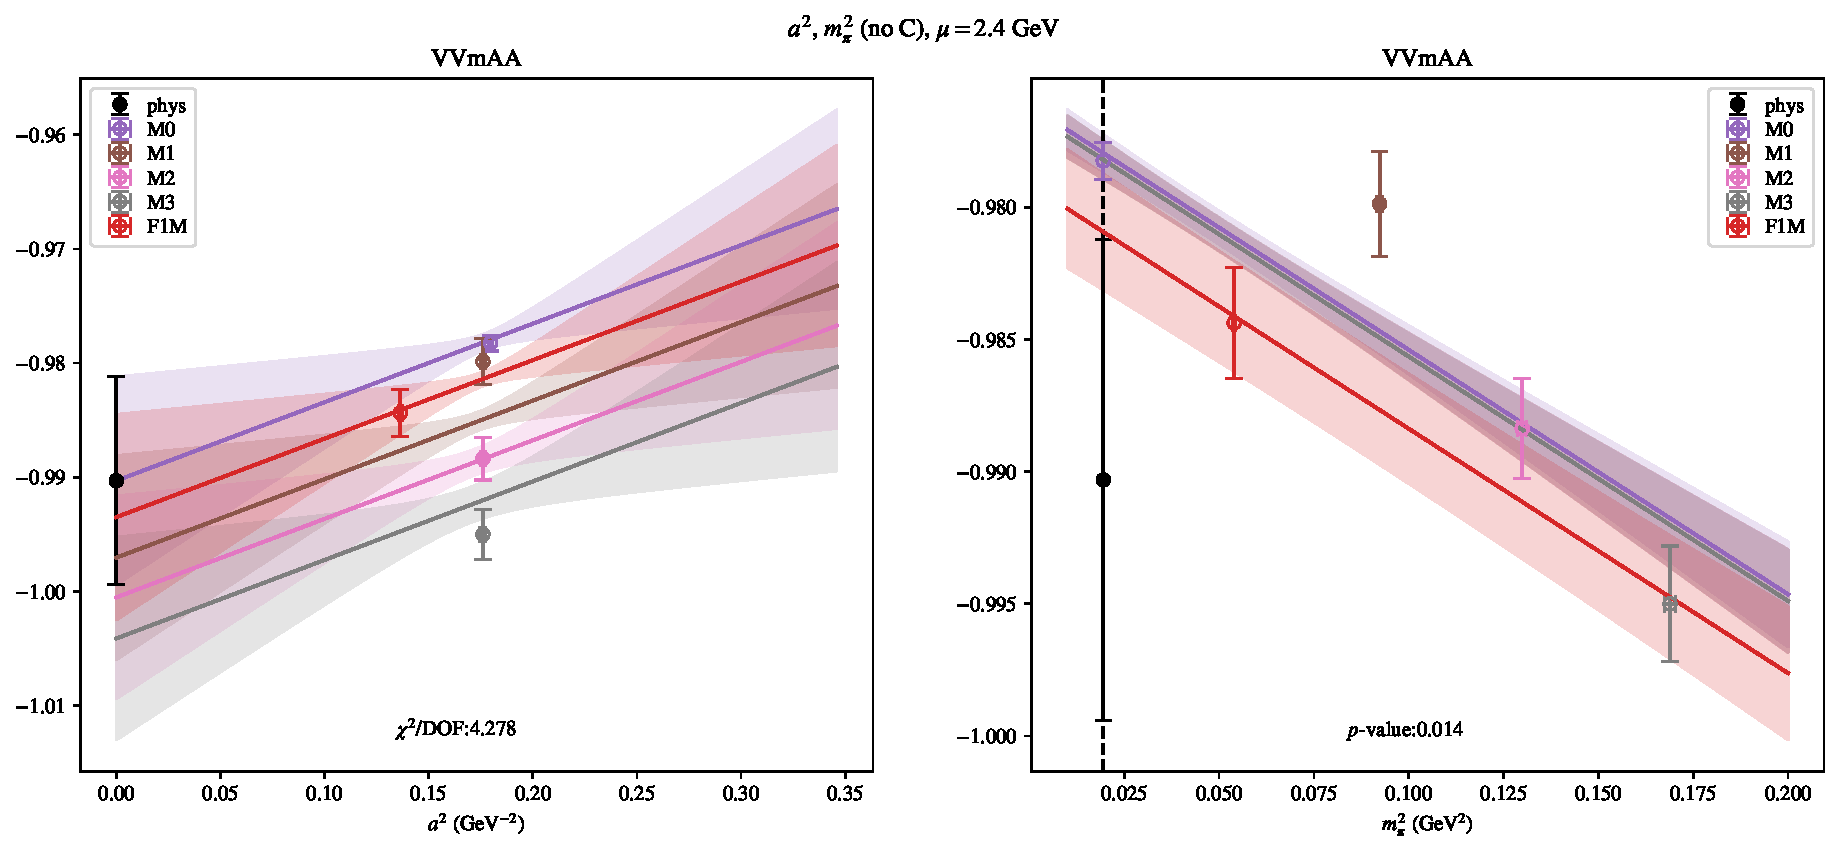
\includepdf[link, pages=-]{VVmAA/NPR/a2m2noC_24.pdf}
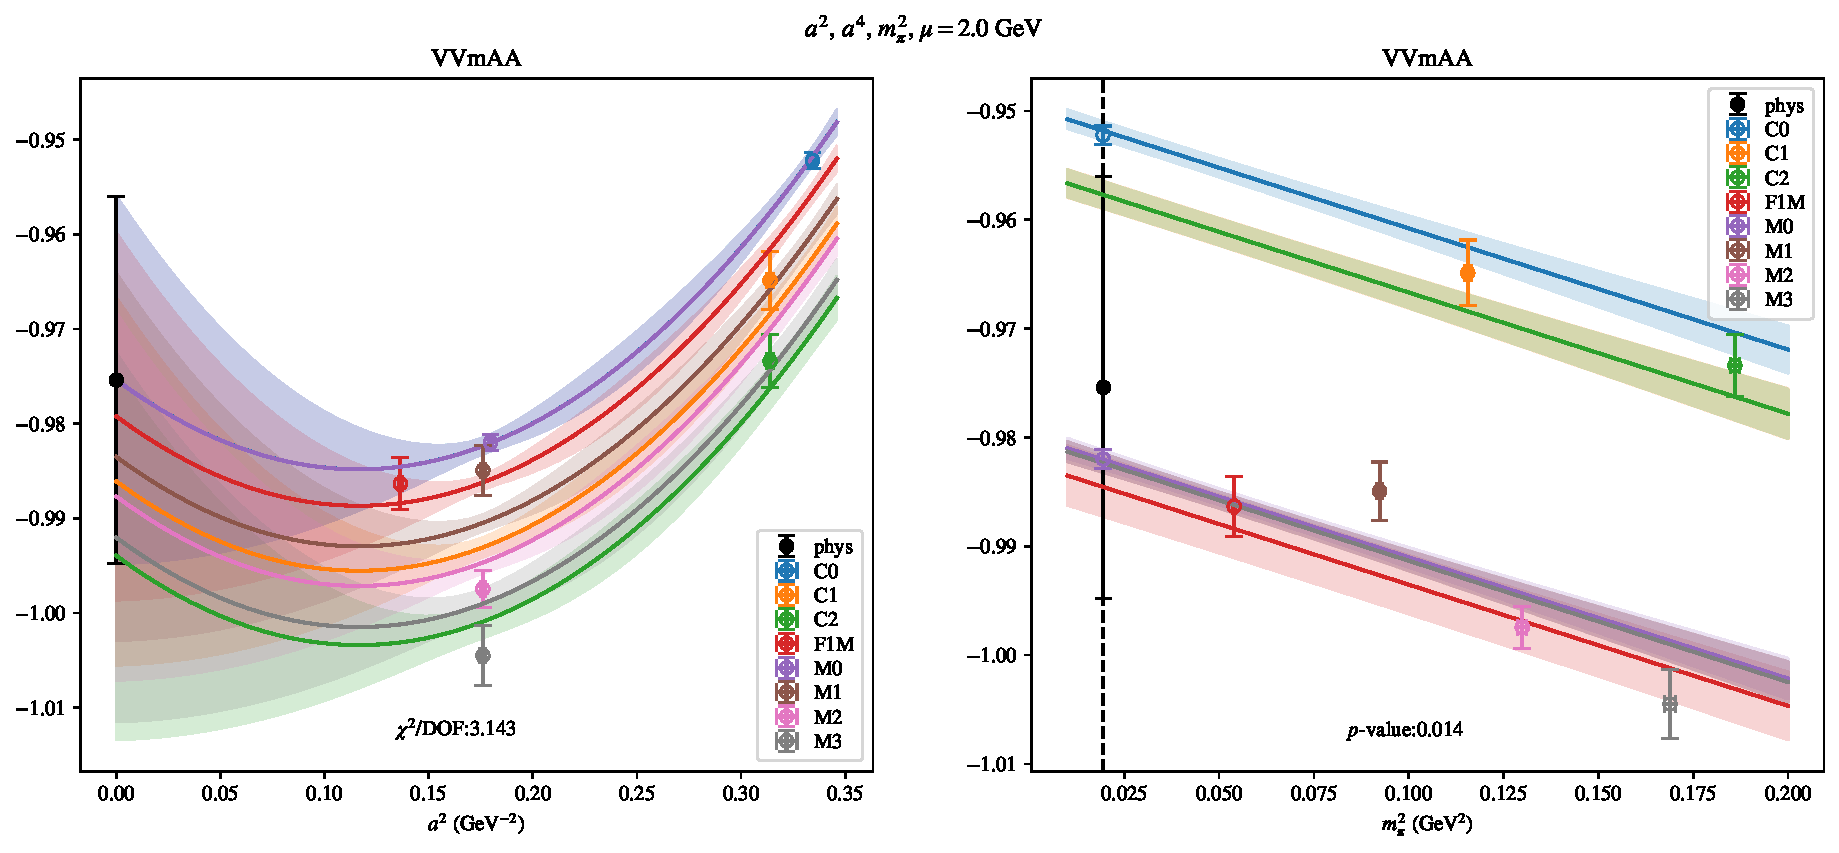
\includepdf[link, pages=-]{VVmAA/NPR/a2a4m2_20.pdf}
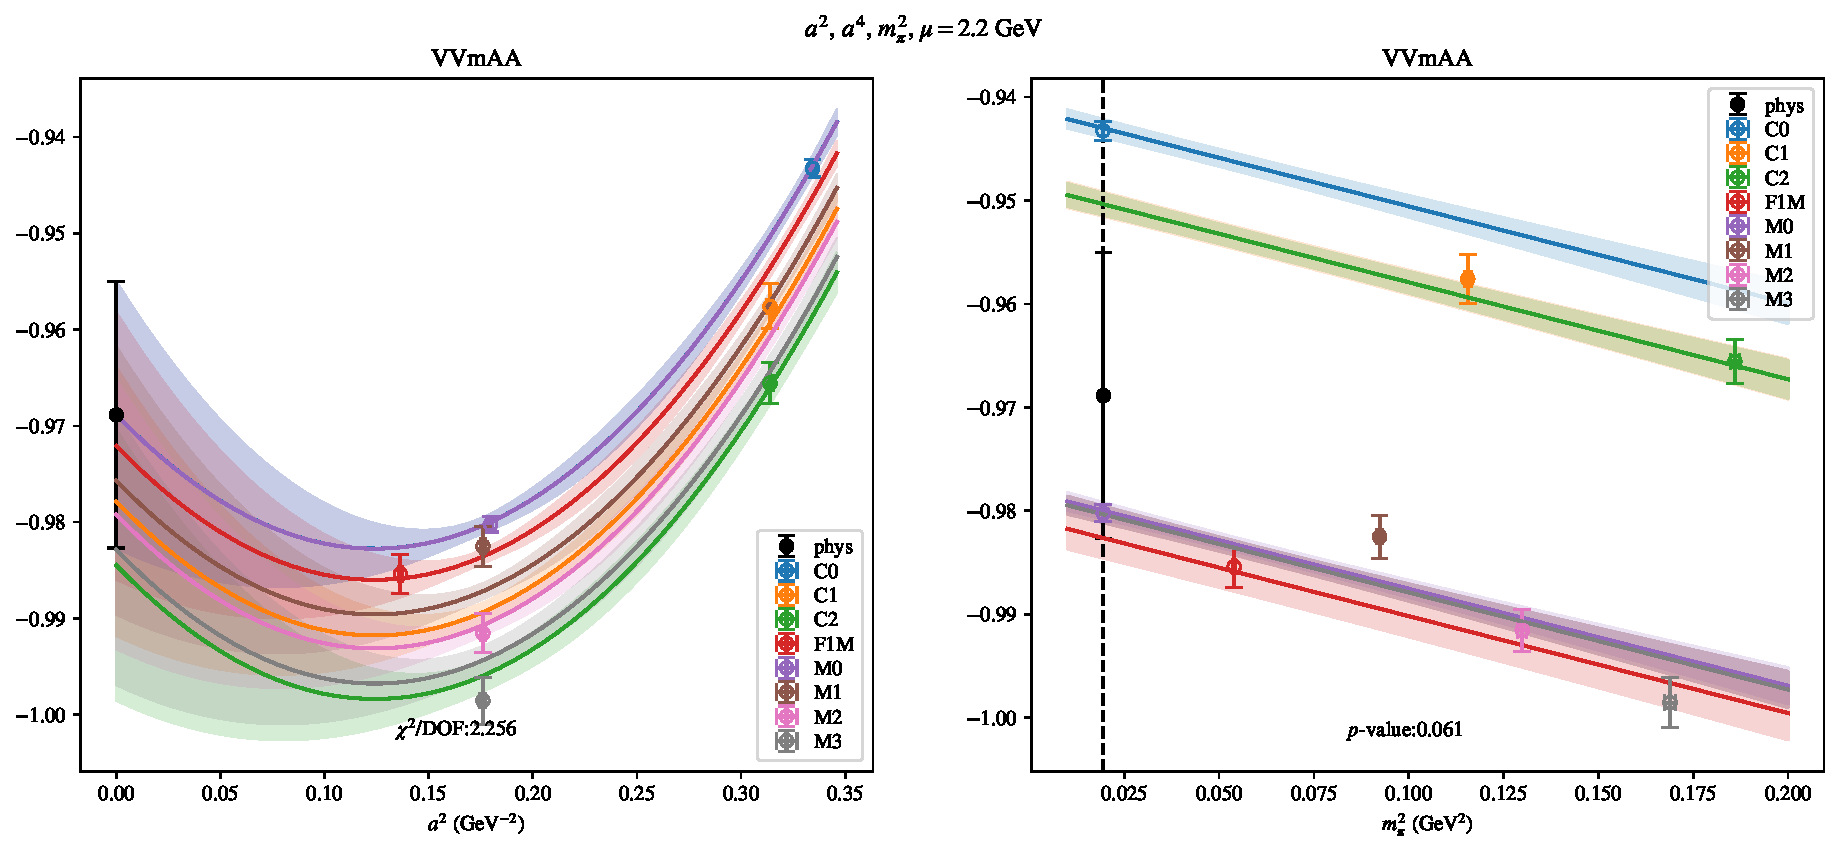
\includepdf[link, pages=-]{VVmAA/NPR/a2a4m2_22.pdf}
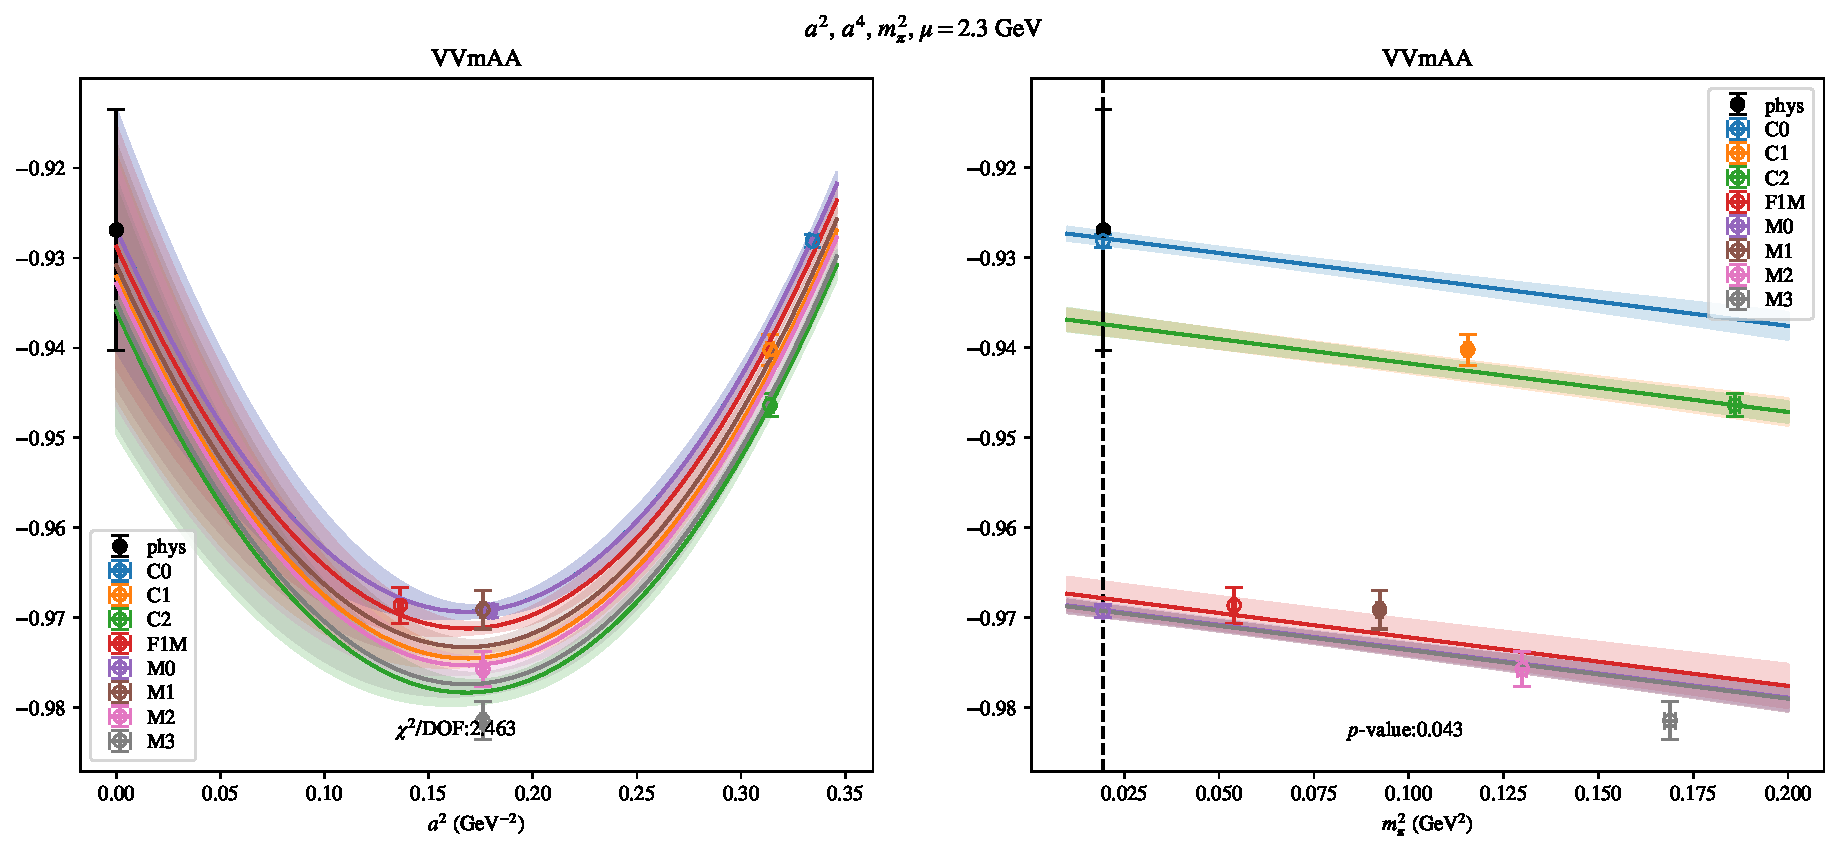
\includepdf[link, pages=-]{VVmAA/NPR/a2a4m2_23.pdf}
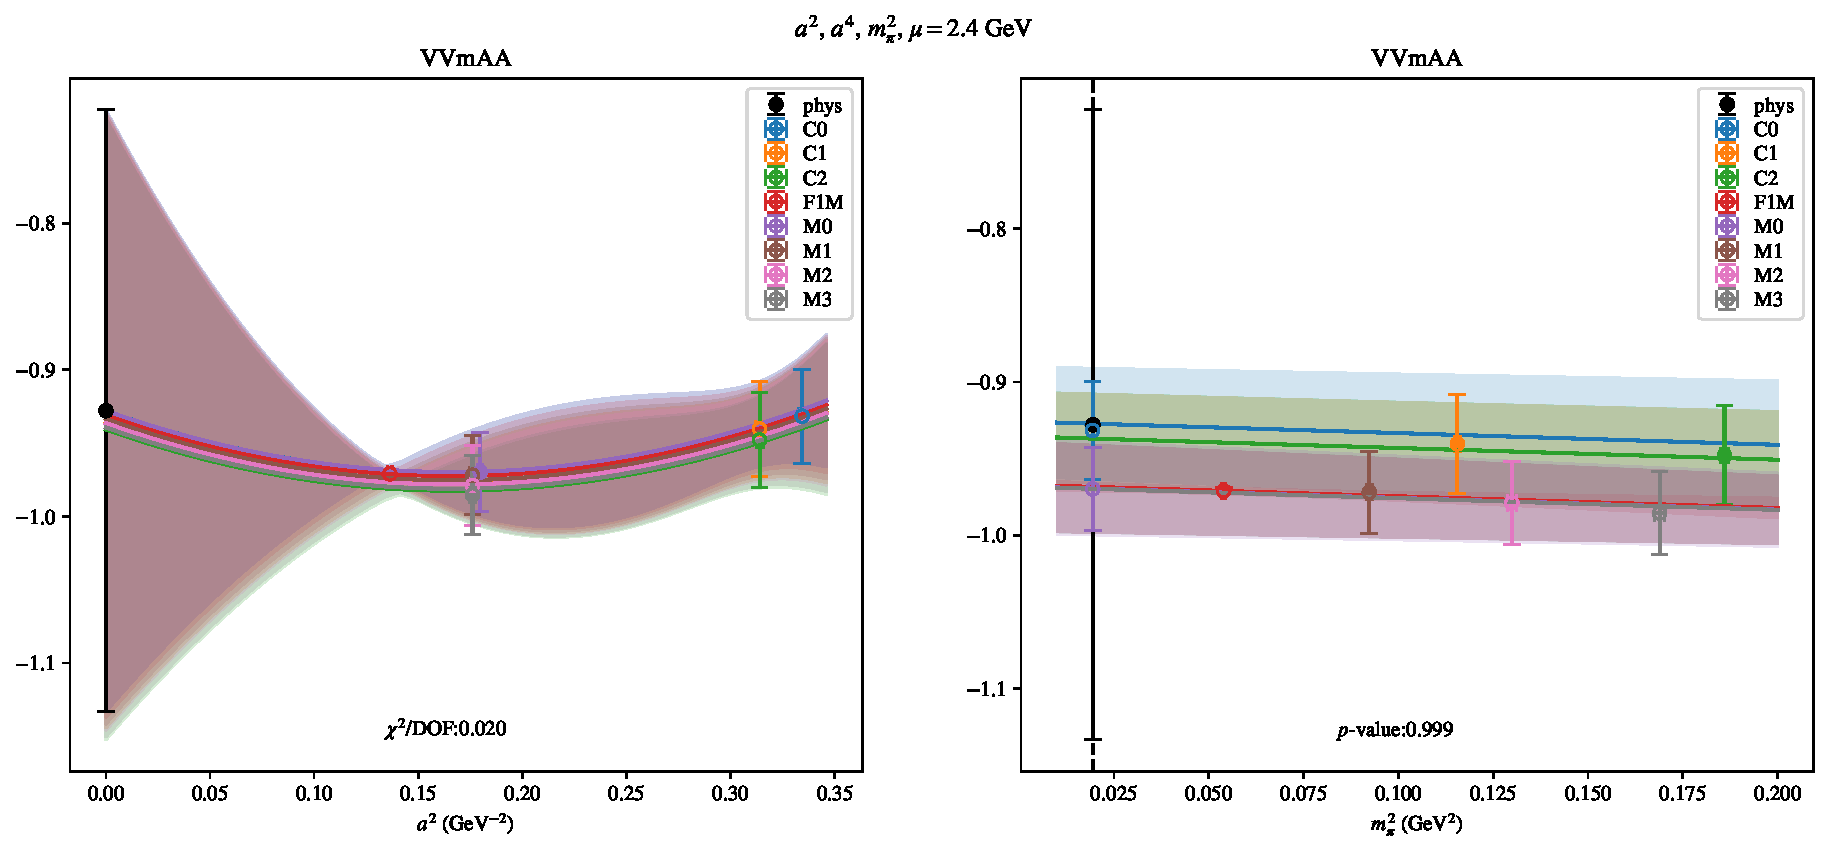
\includepdf[link, pages=-]{VVmAA/NPR/a2a4m2_24.pdf}
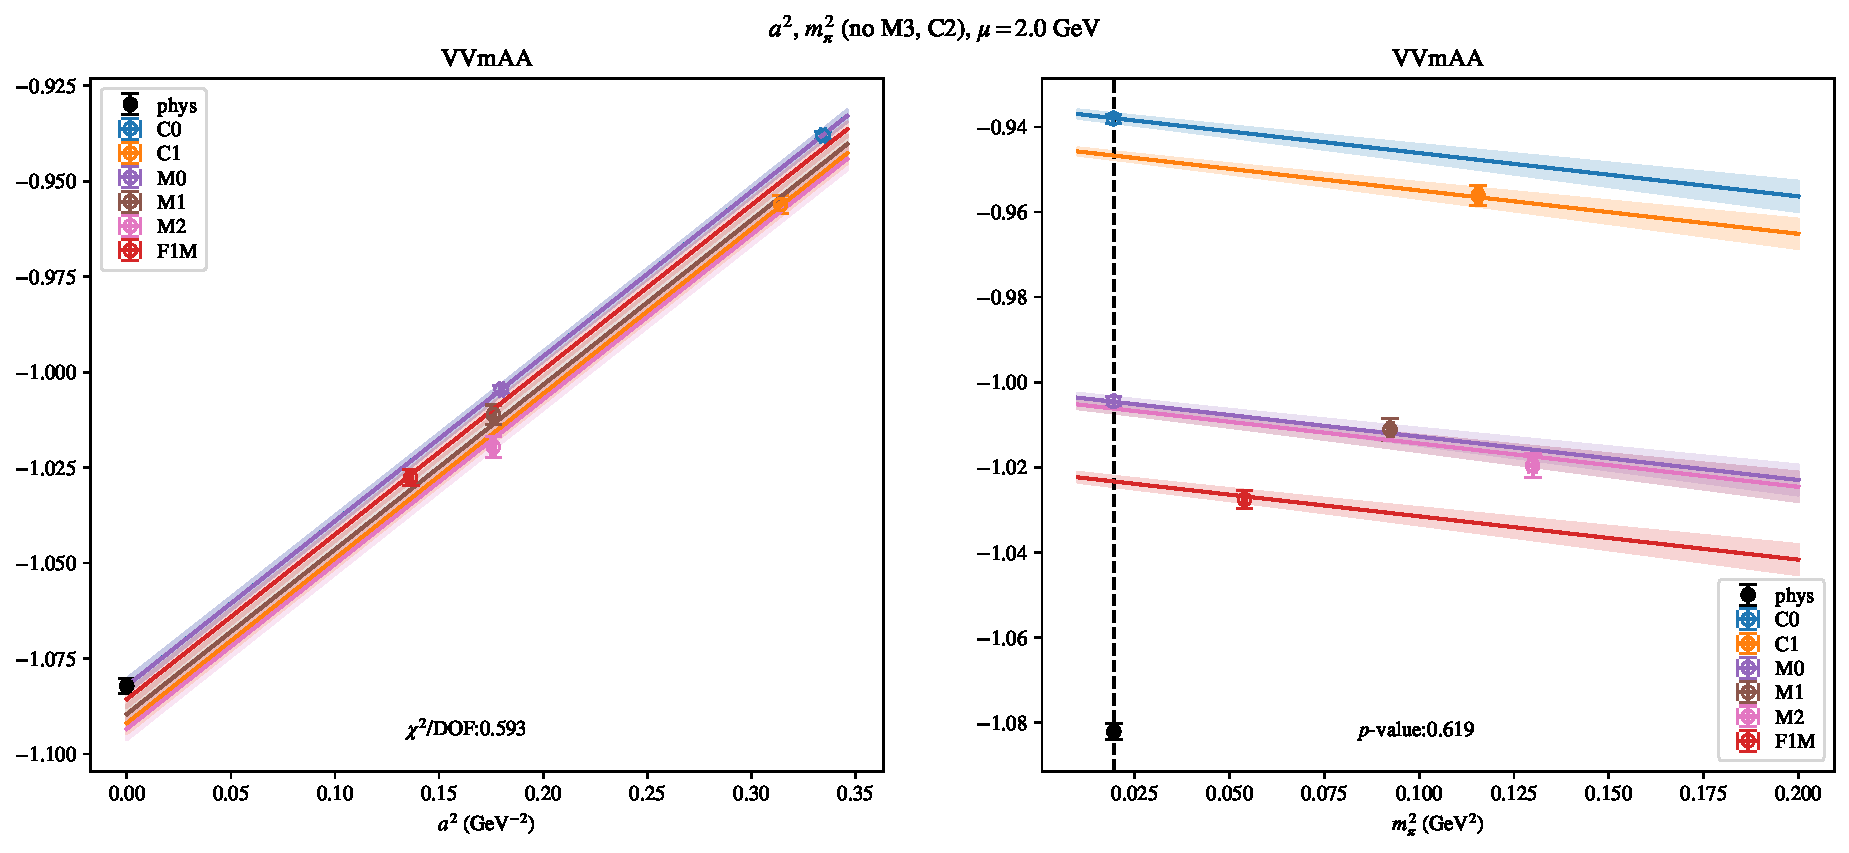
\includepdf[link, pages=-]{VVmAA/NPR/a2m2mcut_20.pdf}
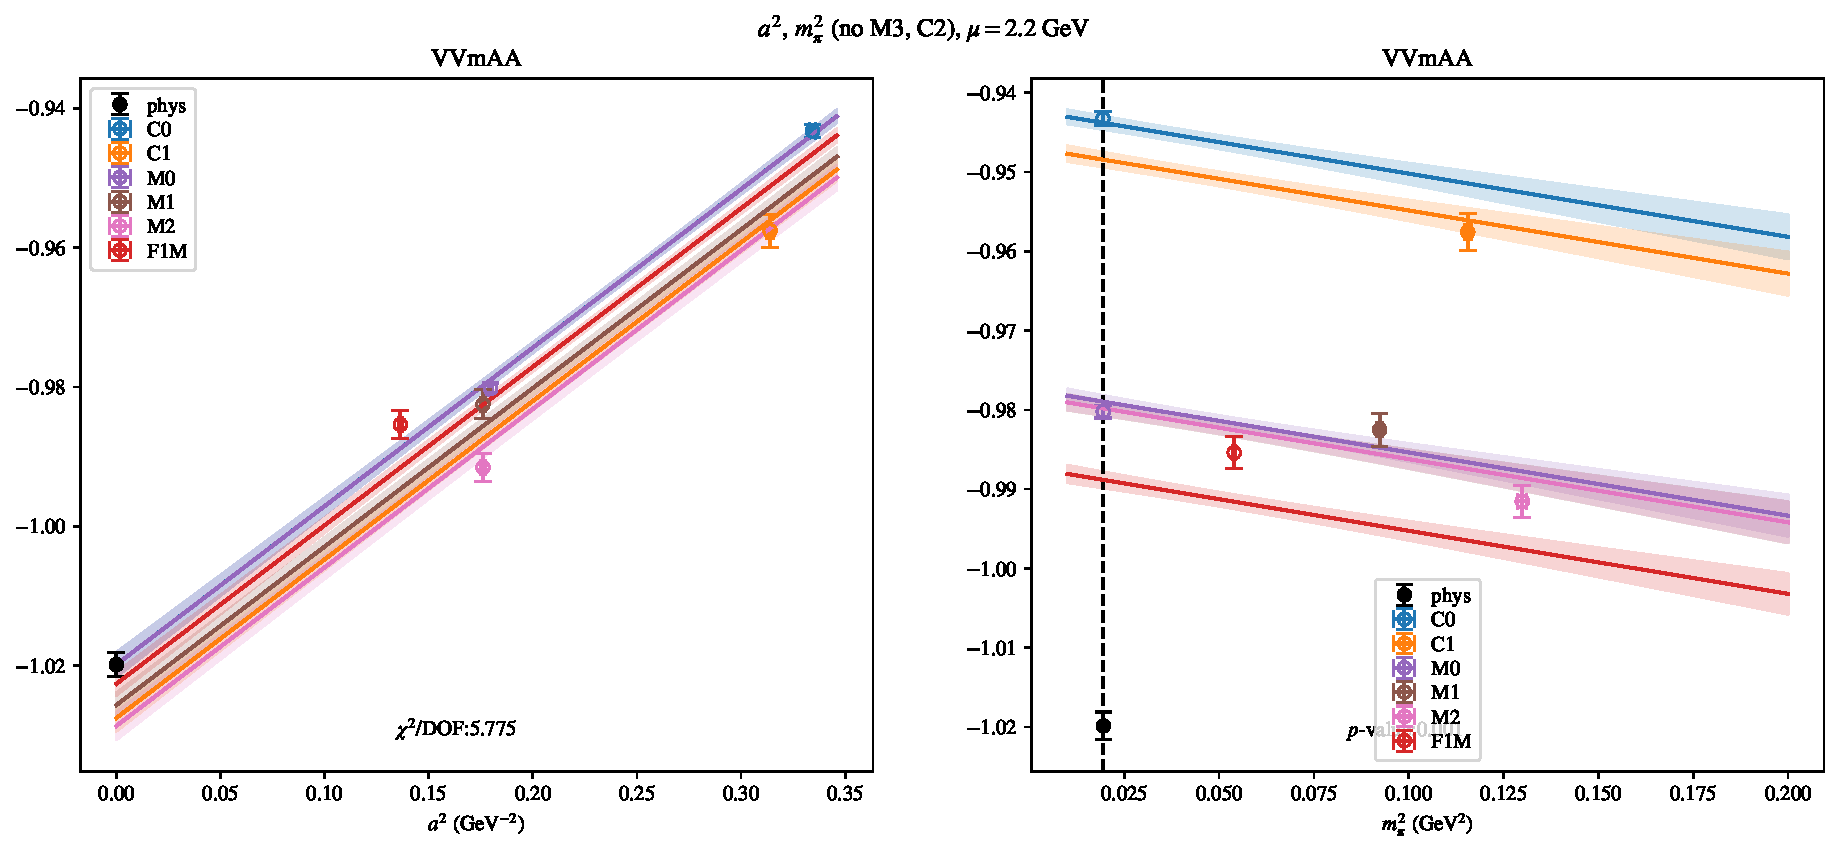
\includepdf[link, pages=-]{VVmAA/NPR/a2m2mcut_22.pdf}
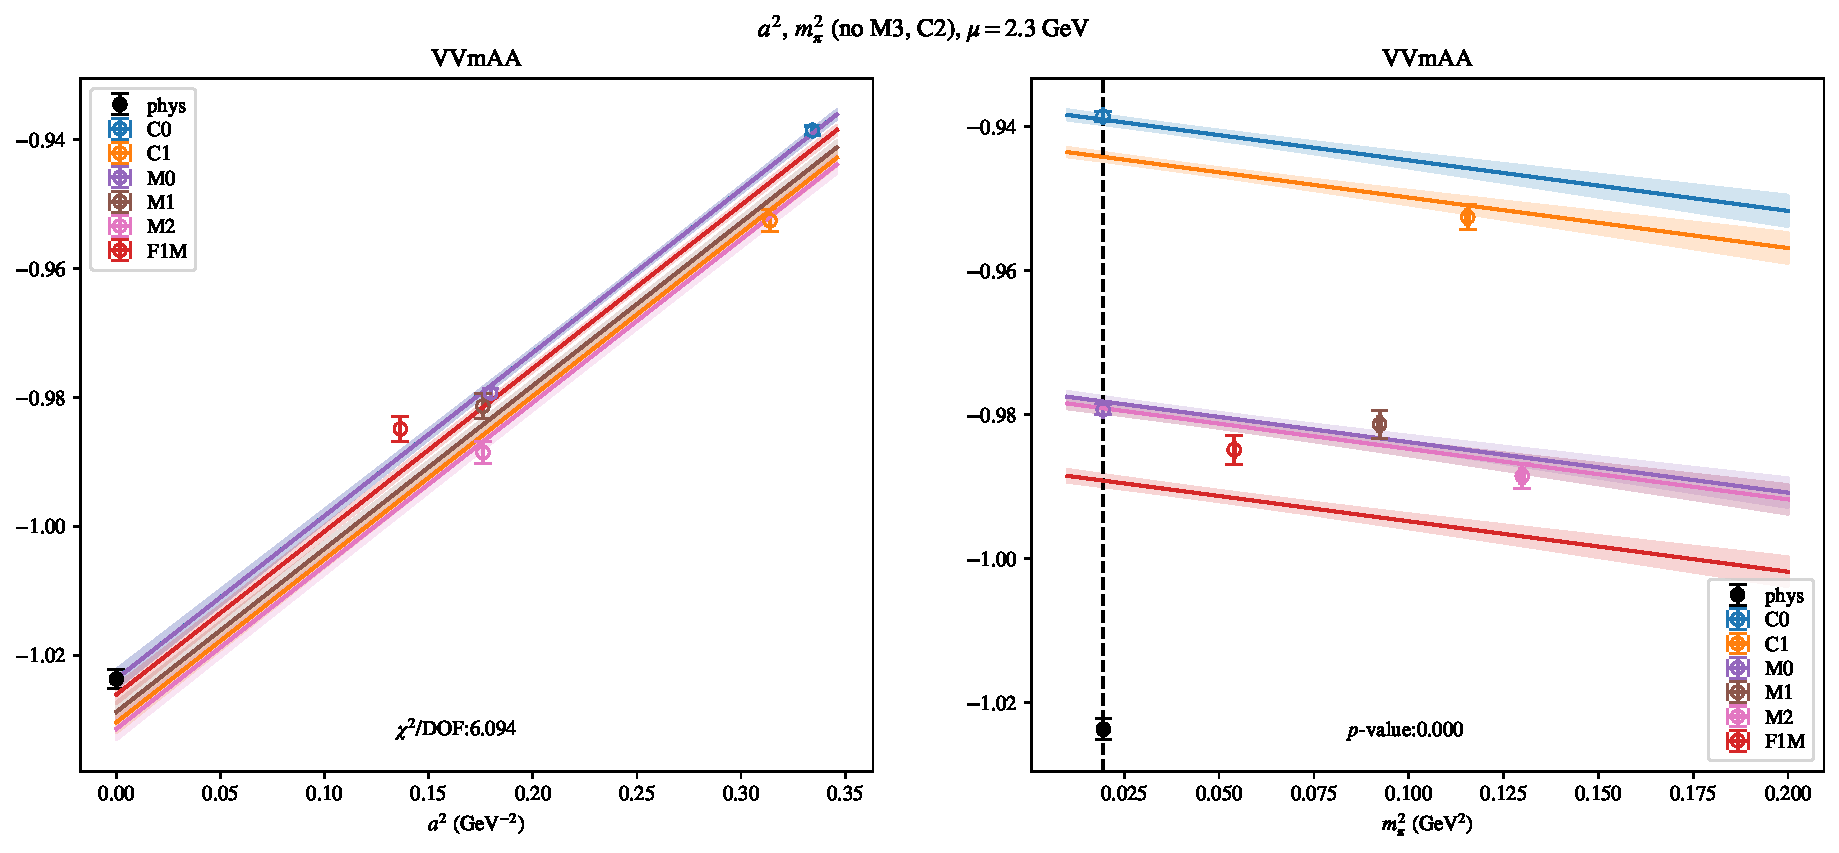
\includepdf[link, pages=-]{VVmAA/NPR/a2m2mcut_23.pdf}
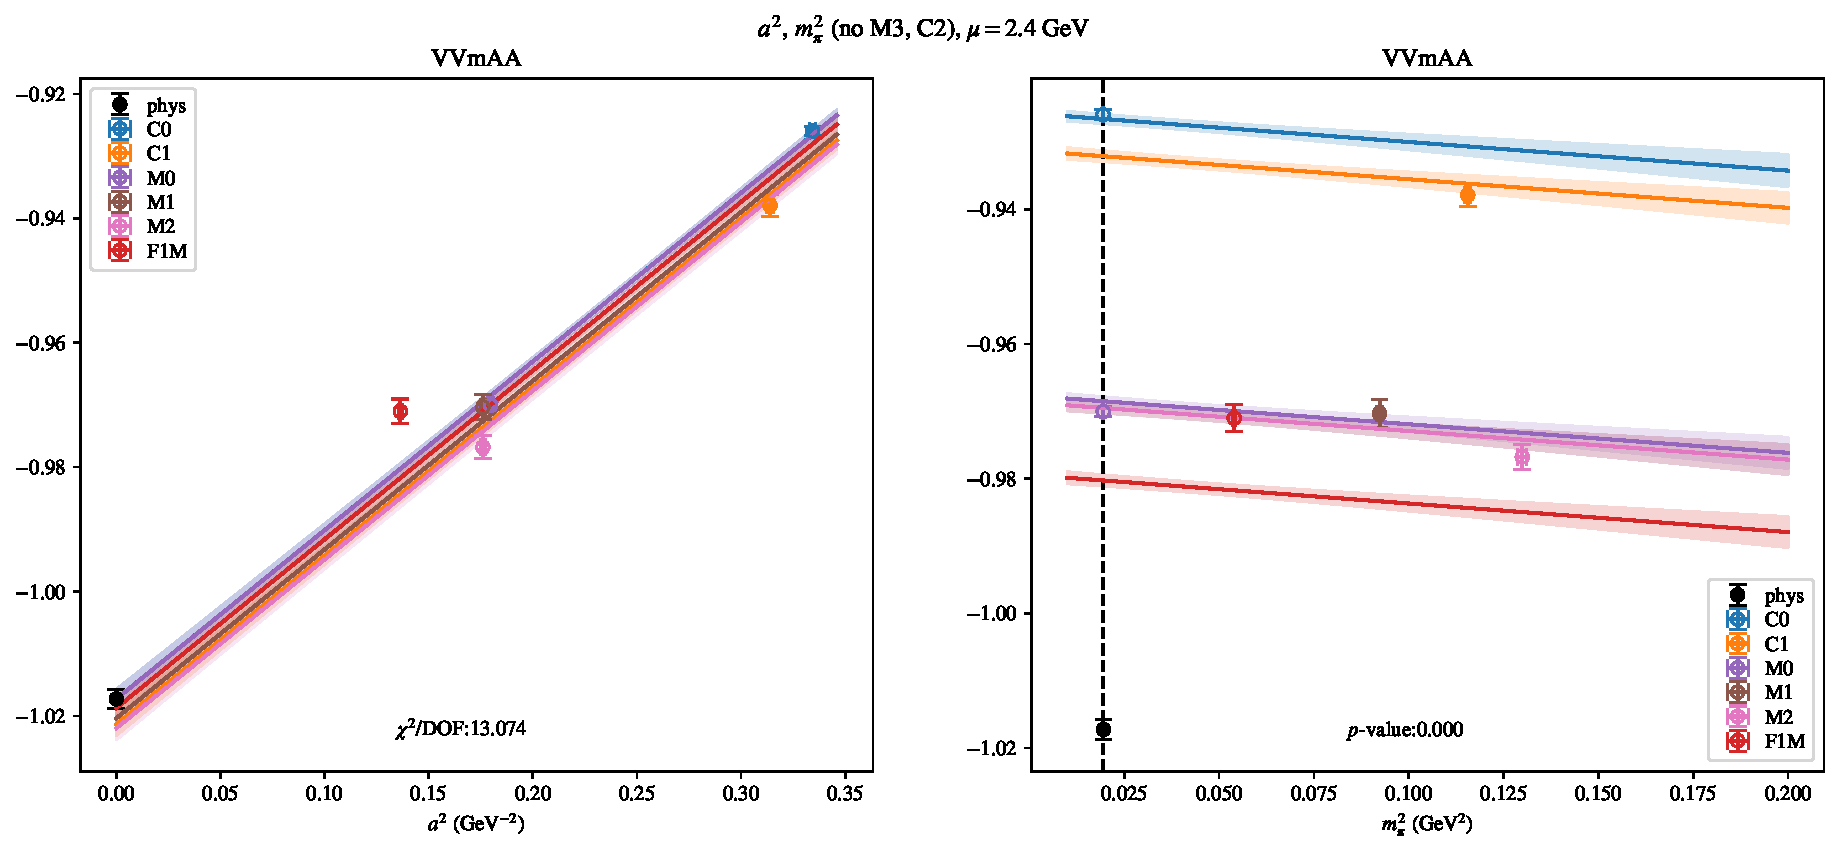
\includepdf[link, pages=-]{VVmAA/NPR/a2m2mcut_24.pdf}
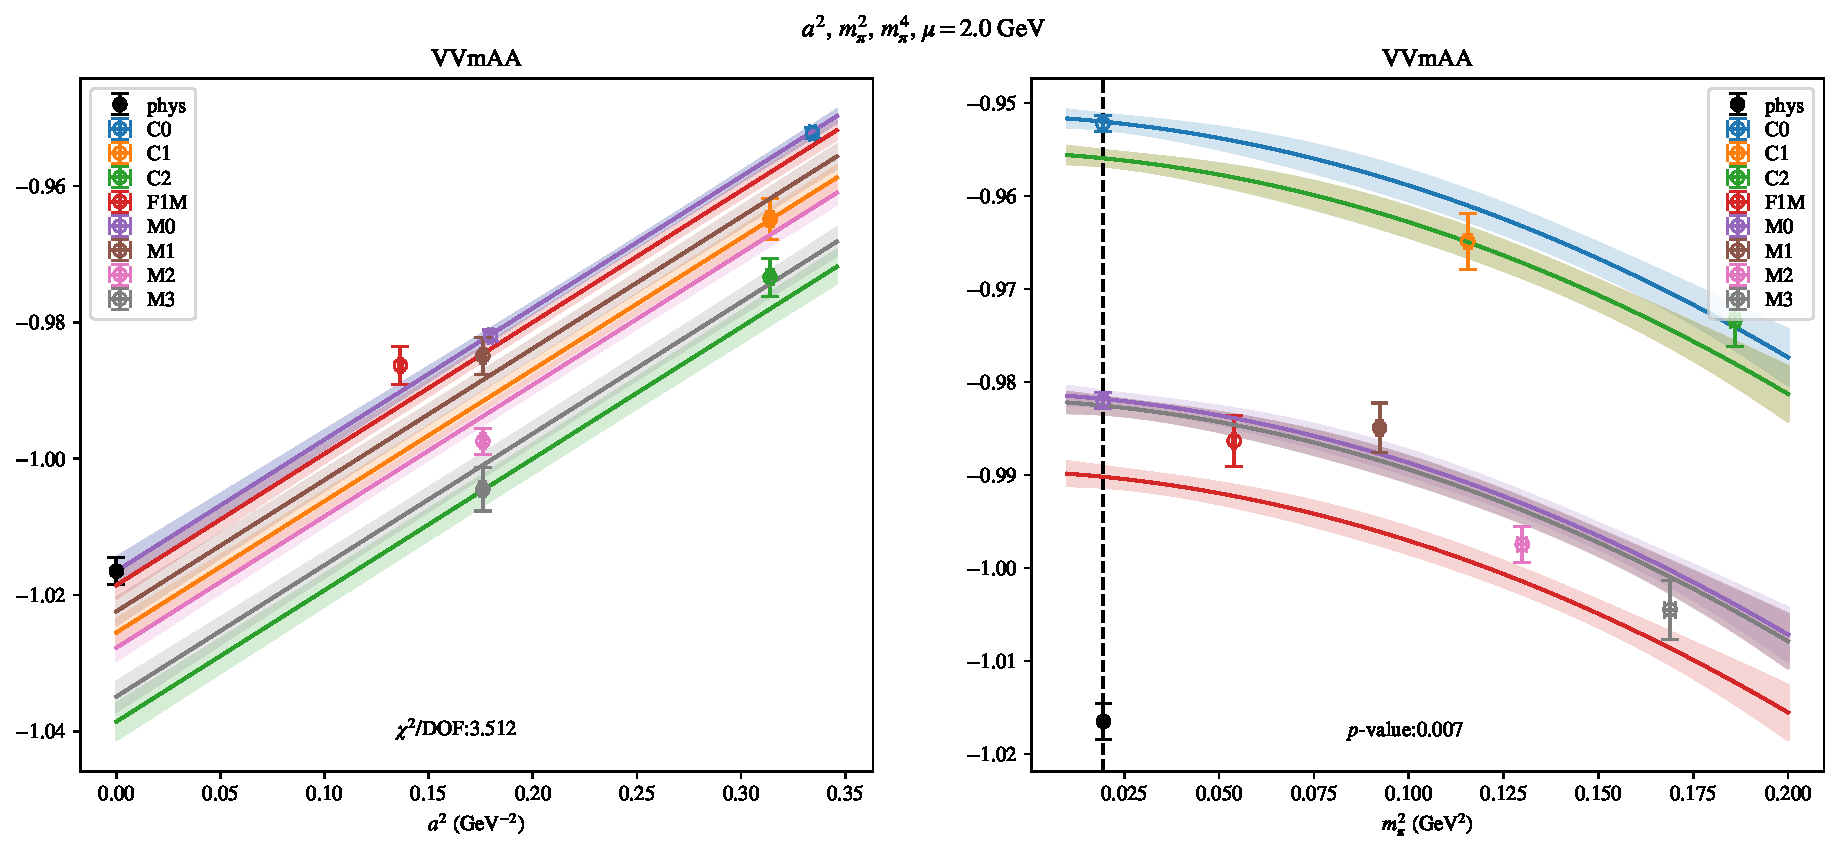
\includepdf[link, pages=-]{VVmAA/NPR/a2m2m4_20.pdf}
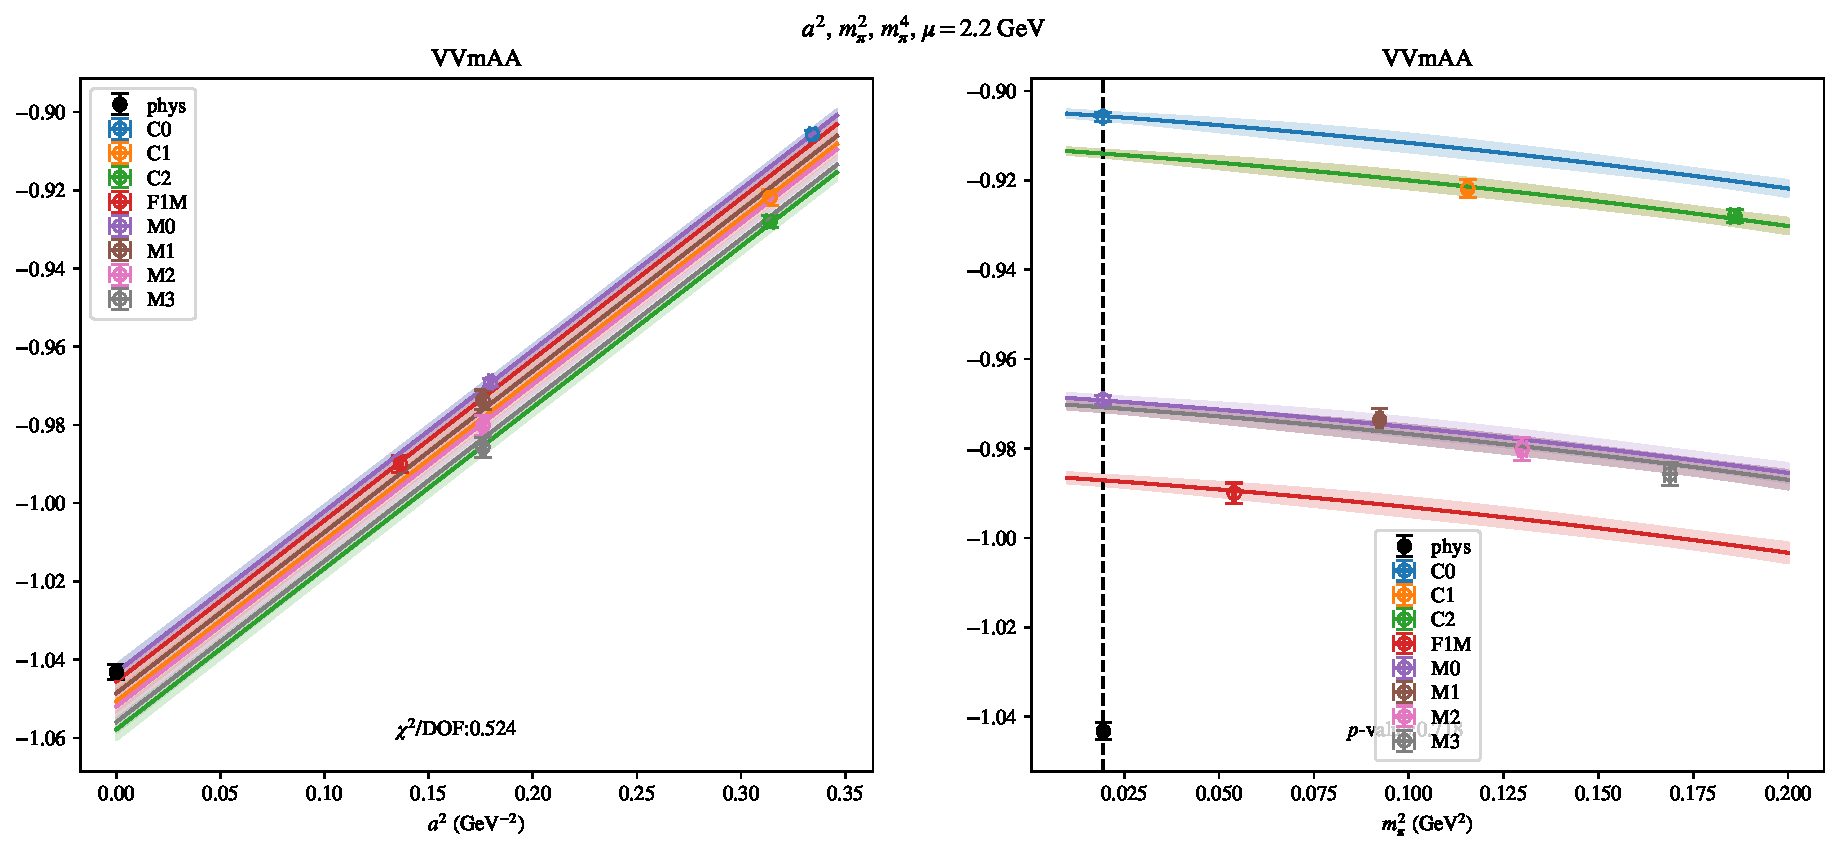
\includepdf[link, pages=-]{VVmAA/NPR/a2m2m4_22.pdf}
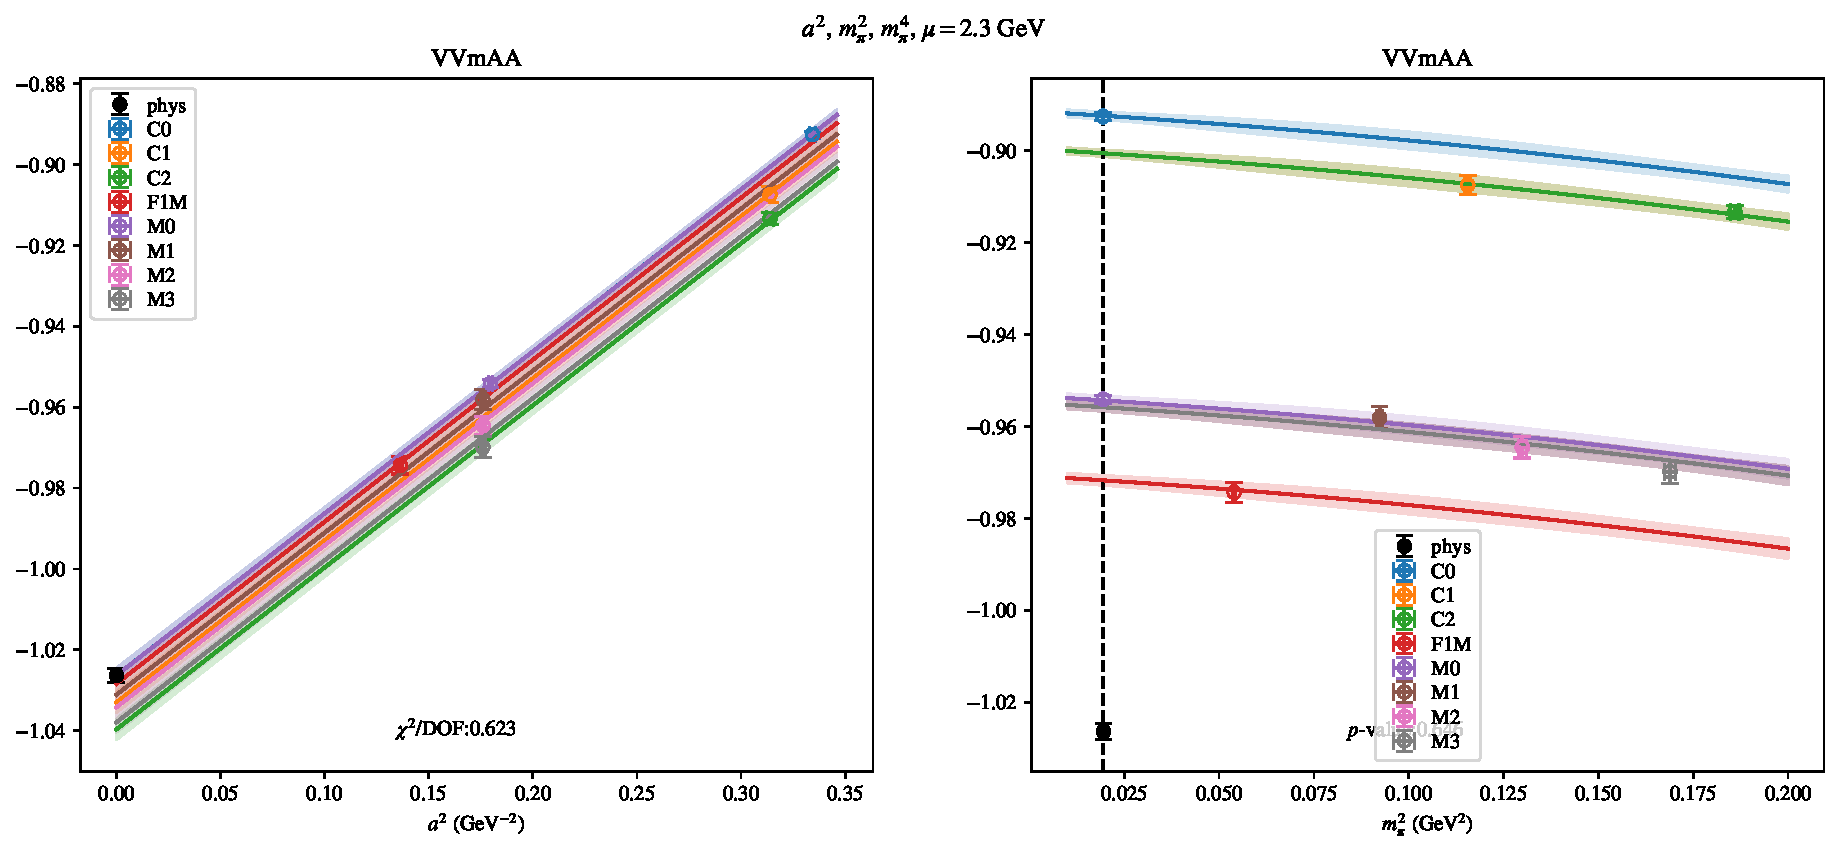
\includepdf[link, pages=-]{VVmAA/NPR/a2m2m4_23.pdf}
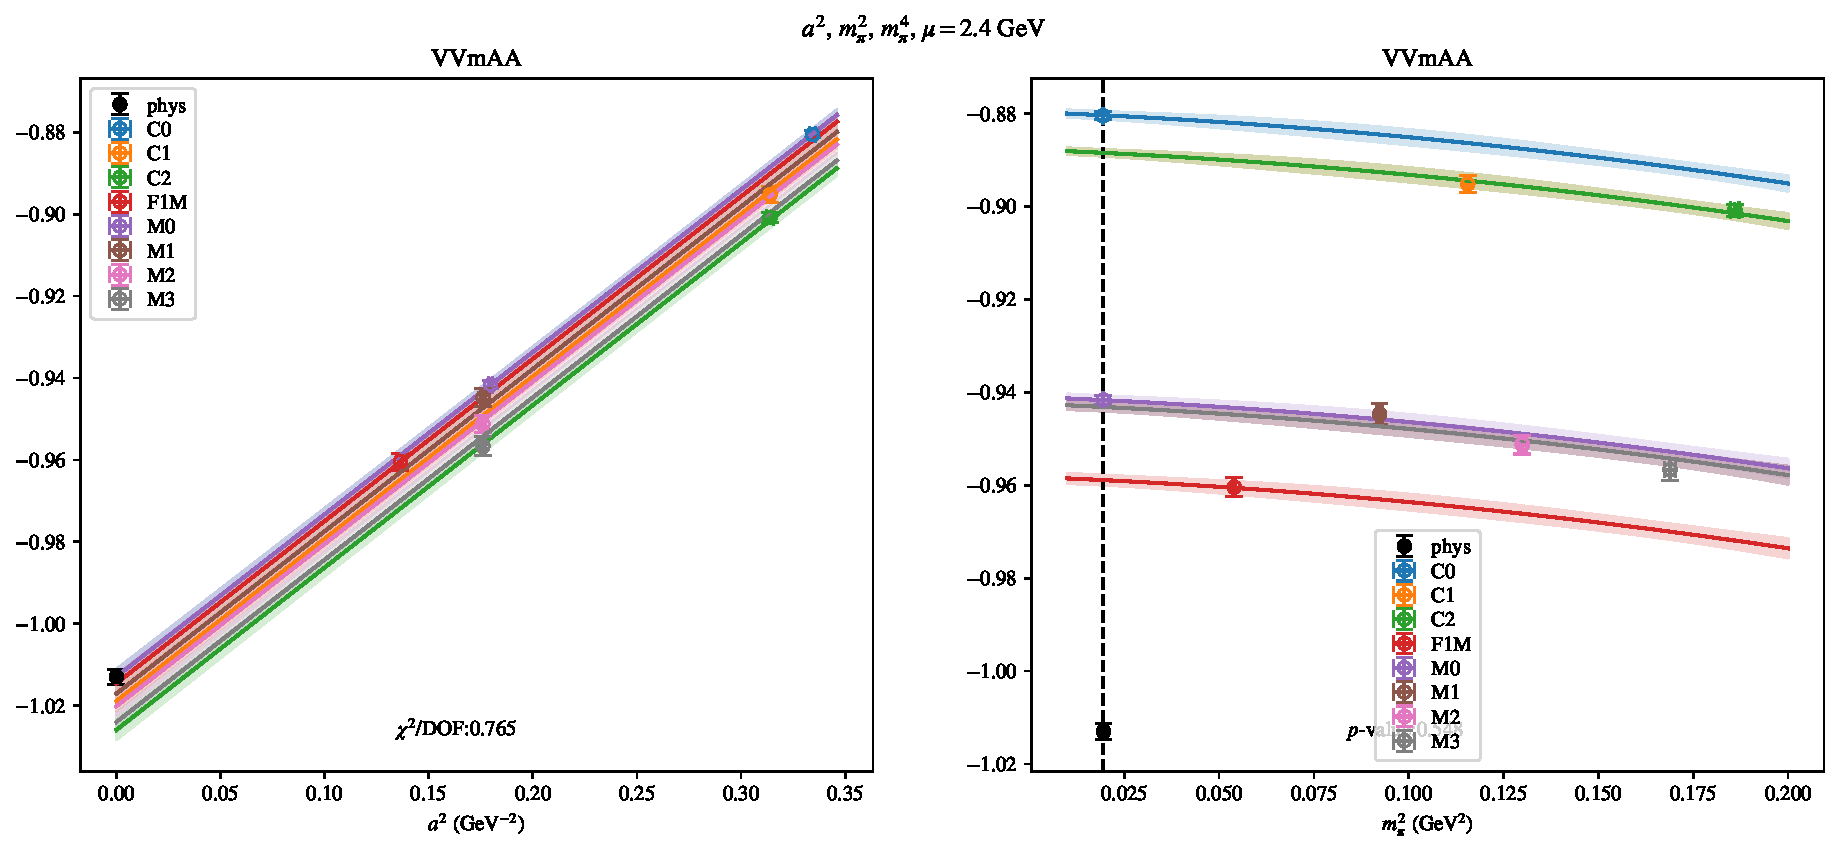
\includepdf[link, pages=-]{VVmAA/NPR/a2m2m4_24.pdf}
\clearpage
\section{$B_3$}
\begin{table}[h!]
\begin{center}
\begin{tabular}{|c|c|c|c|c|c|}
\hline
$\mu$ (GeV) & $a^2$, $m_\pi^2$& $a^2$, $m_\pi^2$ (no C)& $a^2$, $a^4$, $m_\pi^2$& $a^2$, $m_\pi^2$ (no M3, C2)& $a^2$, $m_\pi^2$, $m_\pi^4$\\
\hline
2.0& \hyperlink{SSmPP/NPR/a2m2_20.pdf.1}{\textbf{0.9140(12)}: 5.64 (0.0)} & \hyperlink{SSmPP/NPR/a2m2noC_20.pdf.1}{\textbf{0.8853(65)}: 3.392 (0.034)} & \hyperlink{SSmPP/NPR/a2a4m2_20.pdf.1}{\textbf{0.868(10)}: 2.094 (0.079)} & \hyperlink{SSmPP/NPR/a2m2mcut_20.pdf.1}{\textbf{0.9144(14)}: 7.793 (0.0)} & \hyperlink{SSmPP/NPR/a2m2m4_20.pdf.1}{\textbf{0.9159(14)}: 4.752 (0.001)}\\
2.2& \hyperlink{SSmPP/NPR/a2m2_22.pdf.1}{\textbf{0.9104(12)}: 5.627 (0.0)} & \hyperlink{SSmPP/NPR/a2m2noC_22.pdf.1}{\textbf{0.8803(63)}: 2.059 (0.128)} & \hyperlink{SSmPP/NPR/a2a4m2_22.pdf.1}{\textbf{0.861(10)}: 1.37 (0.242)} & \hyperlink{SSmPP/NPR/a2m2mcut_22.pdf.1}{\textbf{0.9106(13)}: 8.235 (0.0)} & \hyperlink{SSmPP/NPR/a2m2m4_22.pdf.1}{\textbf{0.9121(14)}: 5.199 (0.0)}\\
2.3& \hyperlink{SSmPP/NPR/a2m2_23.pdf.1}{\textbf{0.9090(12)}: 5.971 (0.0)} & \hyperlink{SSmPP/NPR/a2m2noC_23.pdf.1}{\textbf{0.8781(63)}: 2.161 (0.115)} & \hyperlink{SSmPP/NPR/a2a4m2_23.pdf.1}{\textbf{0.859(10)}: 1.532 (0.19)} & \hyperlink{SSmPP/NPR/a2m2mcut_23.pdf.1}{\textbf{0.9093(13)}: 8.74 (0.0)} & \hyperlink{SSmPP/NPR/a2m2m4_23.pdf.1}{\textbf{0.9108(13)}: 5.437 (0.0)}\\
2.4& \hyperlink{SSmPP/NPR/a2m2_24.pdf.1}{\textbf{0.9080(12)}: 6.697 (0.0)} & \hyperlink{SSmPP/NPR/a2m2noC_24.pdf.1}{\textbf{0.8757(62)}: 2.496 (0.082)} & \hyperlink{SSmPP/NPR/a2a4m2_24.pdf.1}{\textbf{0.8559(99)}: 1.713 (0.144)} & \hyperlink{SSmPP/NPR/a2m2mcut_24.pdf.1}{\textbf{0.9084(13)}: 9.824 (0.0)} & \hyperlink{SSmPP/NPR/a2m2m4_24.pdf.1}{\textbf{0.9100(13)}: 6.06 (0.0)}\\
\hline
\end{tabular}
\caption{Physical point value from chiral and continuum extrapolation at renormalisation scale $\mu$. Entries are \textbf{value(error)}: $\chi^2/\text{DOF}$ ($p$-value).}
\end{center}
\end{table}
\begin{table}[h!]
\begin{center}
\begin{tabular}{|c c|c|c|c|c|c|}
\hline
$\mu$ (GeV) &  & $a^2$, $m_\pi^2$& $a^2$, $m_\pi^2$ (no C)& $a^2$, $a^4$, $m_\pi^2$& $a^2$, $m_\pi^2$ (no M3, C2)& $a^2$, $m_\pi^2$, $m_\pi^4$\\
\hline
\multirow{2}{0.5in}{2.0} & $\alpha$ & 0.0556(54)& 0.246(43)& 0.53(11)& 0.0548(60)& 0.0486(59)\\
 & $\beta$ & 0.0& 0.0& -0.0001(14)& -0.0002(23)& -0.0019(63)\\
\hline
\multirow{2}{0.5in}{2.2} & $\alpha$ & 0.0542(53)& 0.254(42)& 0.56(11)& 0.0537(57)& 0.0480(58)\\
 & $\beta$ & -0.0002(12)& -0.0002(22)& -0.0004(13)& -0.0005(23)& -0.0019(66)\\
\hline
\multirow{2}{0.5in}{2.3} & $\alpha$ & 0.0544(52)& 0.261(42)& 0.57(11)& 0.0536(57)& 0.0477(57)\\
 & $\beta$ & -0.0003(11)& -0.0003(21)& -0.0005(13)& -0.0005(22)& -0.0020(64)\\
\hline
\multirow{2}{0.5in}{2.4} & $\alpha$ & 0.0540(52)& 0.271(42)& 0.60(11)& 0.0529(57)& 0.0468(57)\\
 & $\beta$ & -0.0003(11)& -0.0003(20)& -0.0005(12)& -0.0006(20)& -0.0022(62)\\
\hline
\end{tabular}
\caption{Fit values of coefficients in $B = B_{phys} + \mathbf{\alpha} a^2 + \mathbf{\beta}\left(\frac{m_\pi^2}{f_\pi^2}-\frac{m_{\pi,PDG}^2}{f_\pi^2}\right) + \ldots$.}
\end{center}
\end{table}
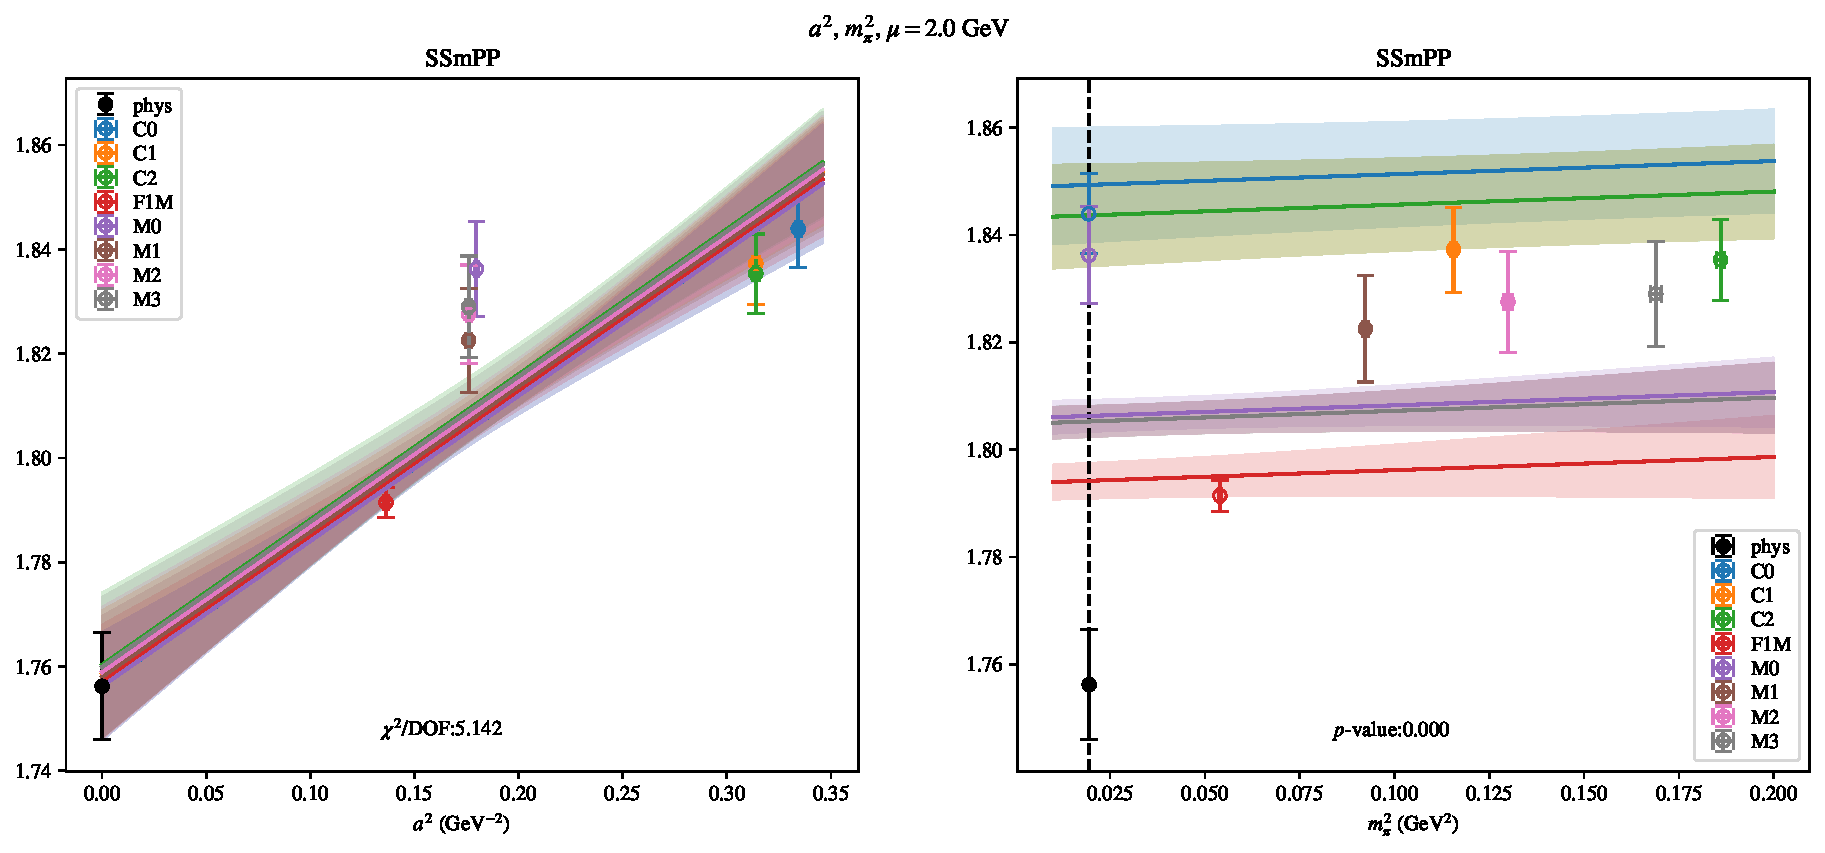
\includepdf[link, pages=-]{SSmPP/NPR/a2m2_20.pdf}
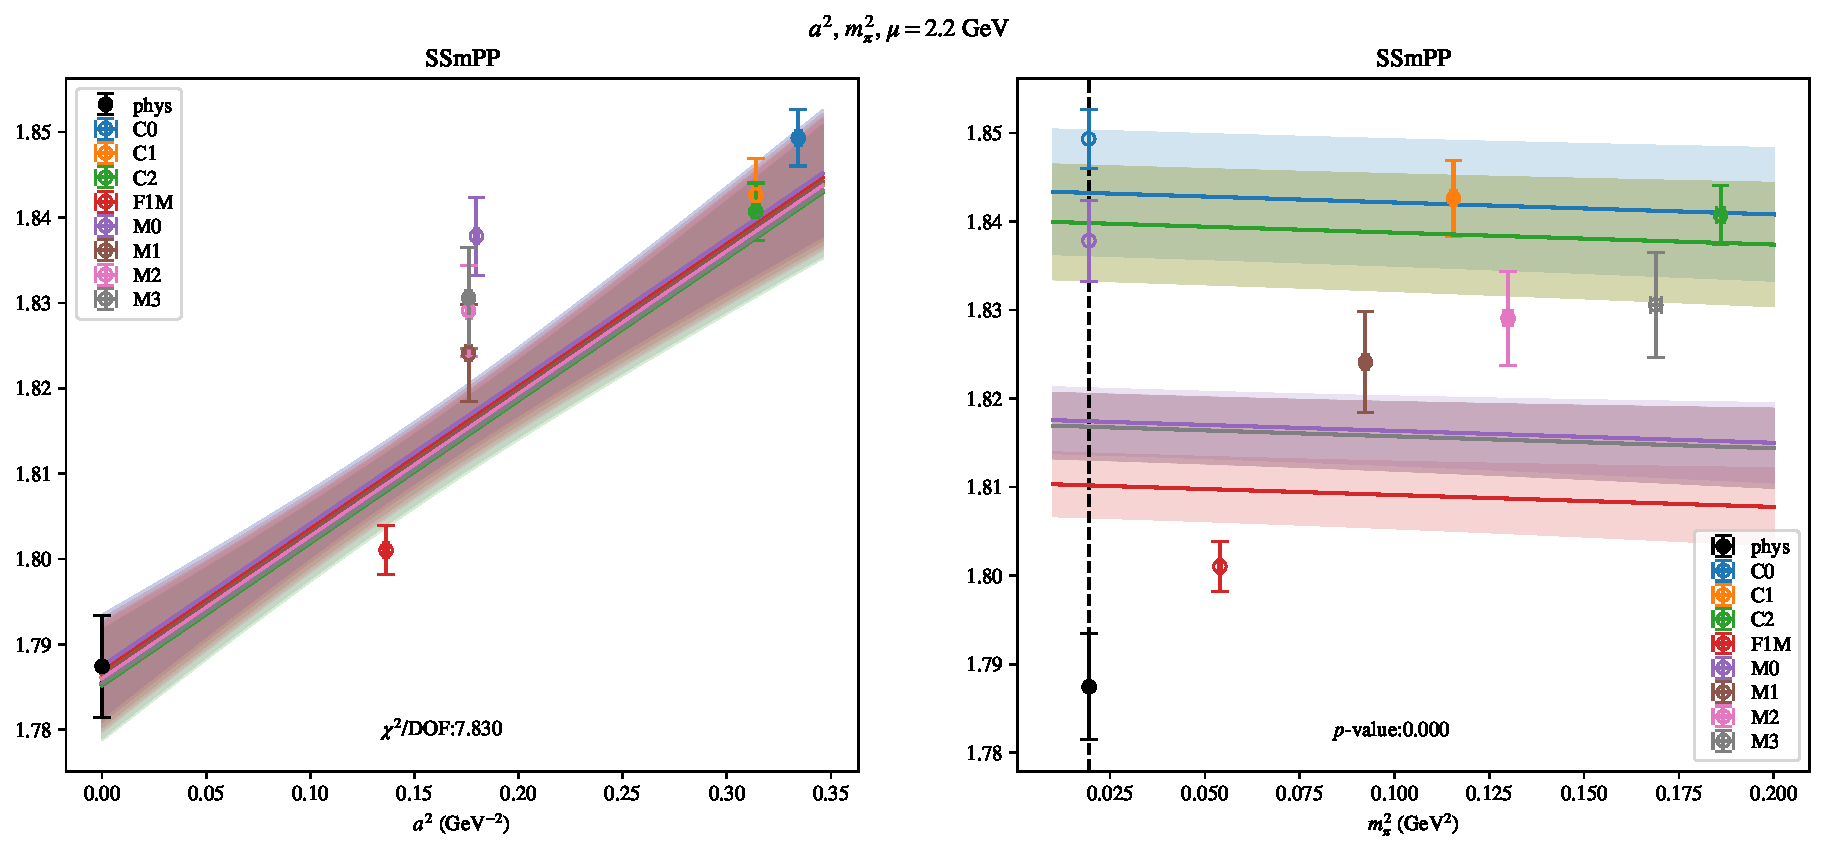
\includepdf[link, pages=-]{SSmPP/NPR/a2m2_22.pdf}
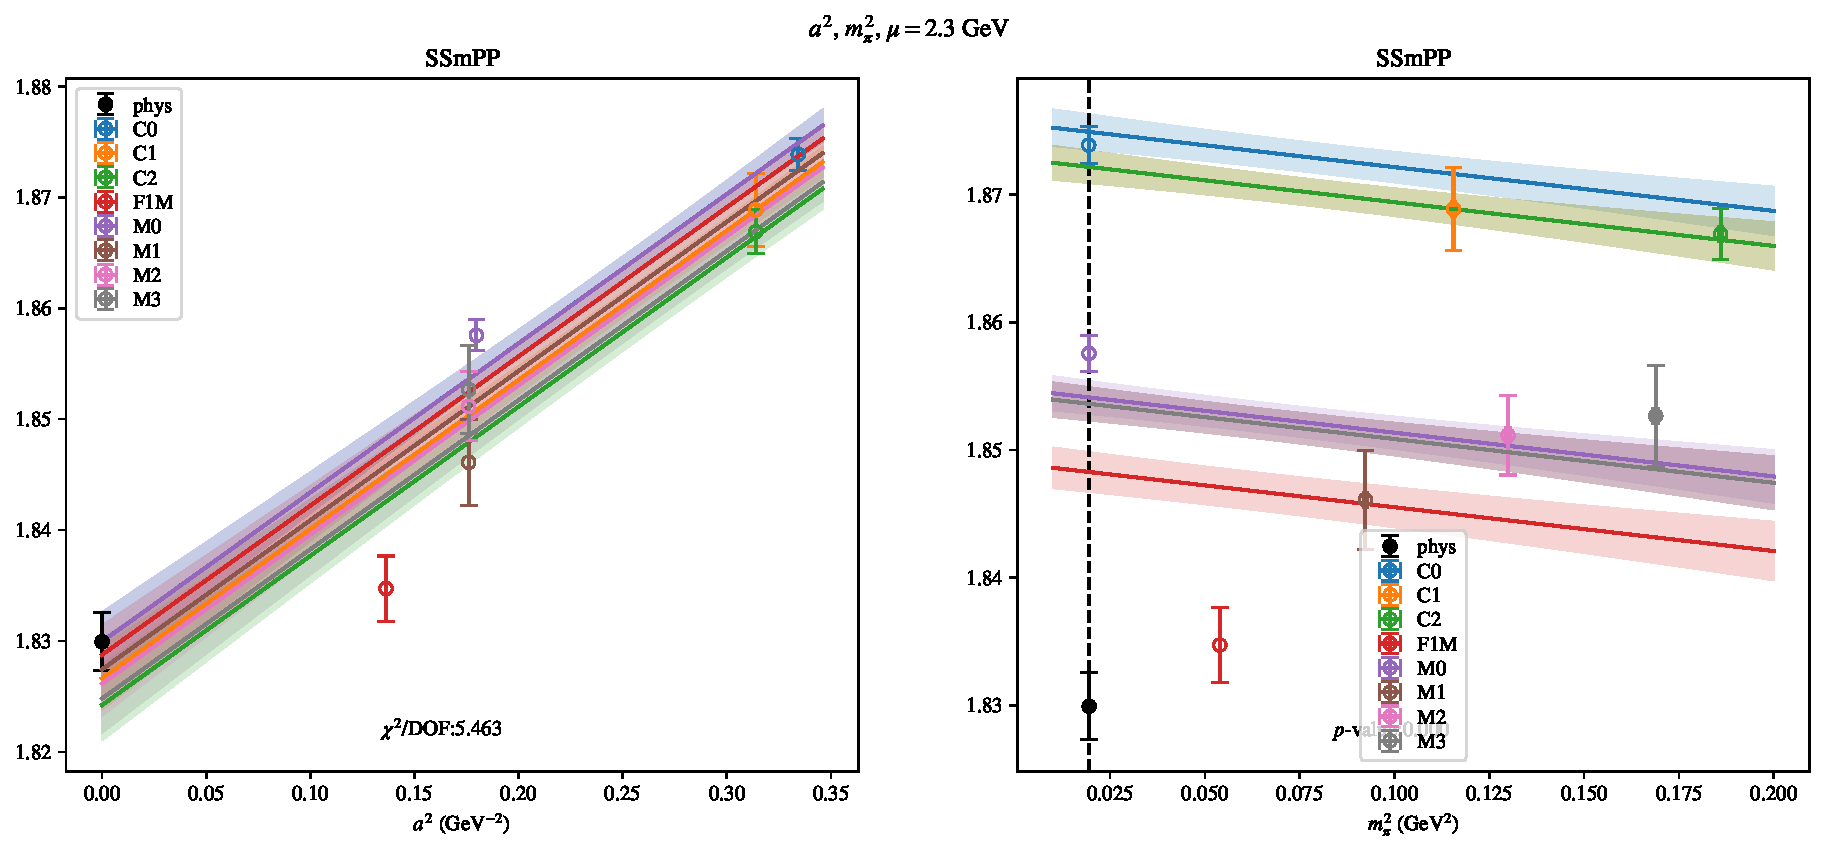
\includepdf[link, pages=-]{SSmPP/NPR/a2m2_23.pdf}
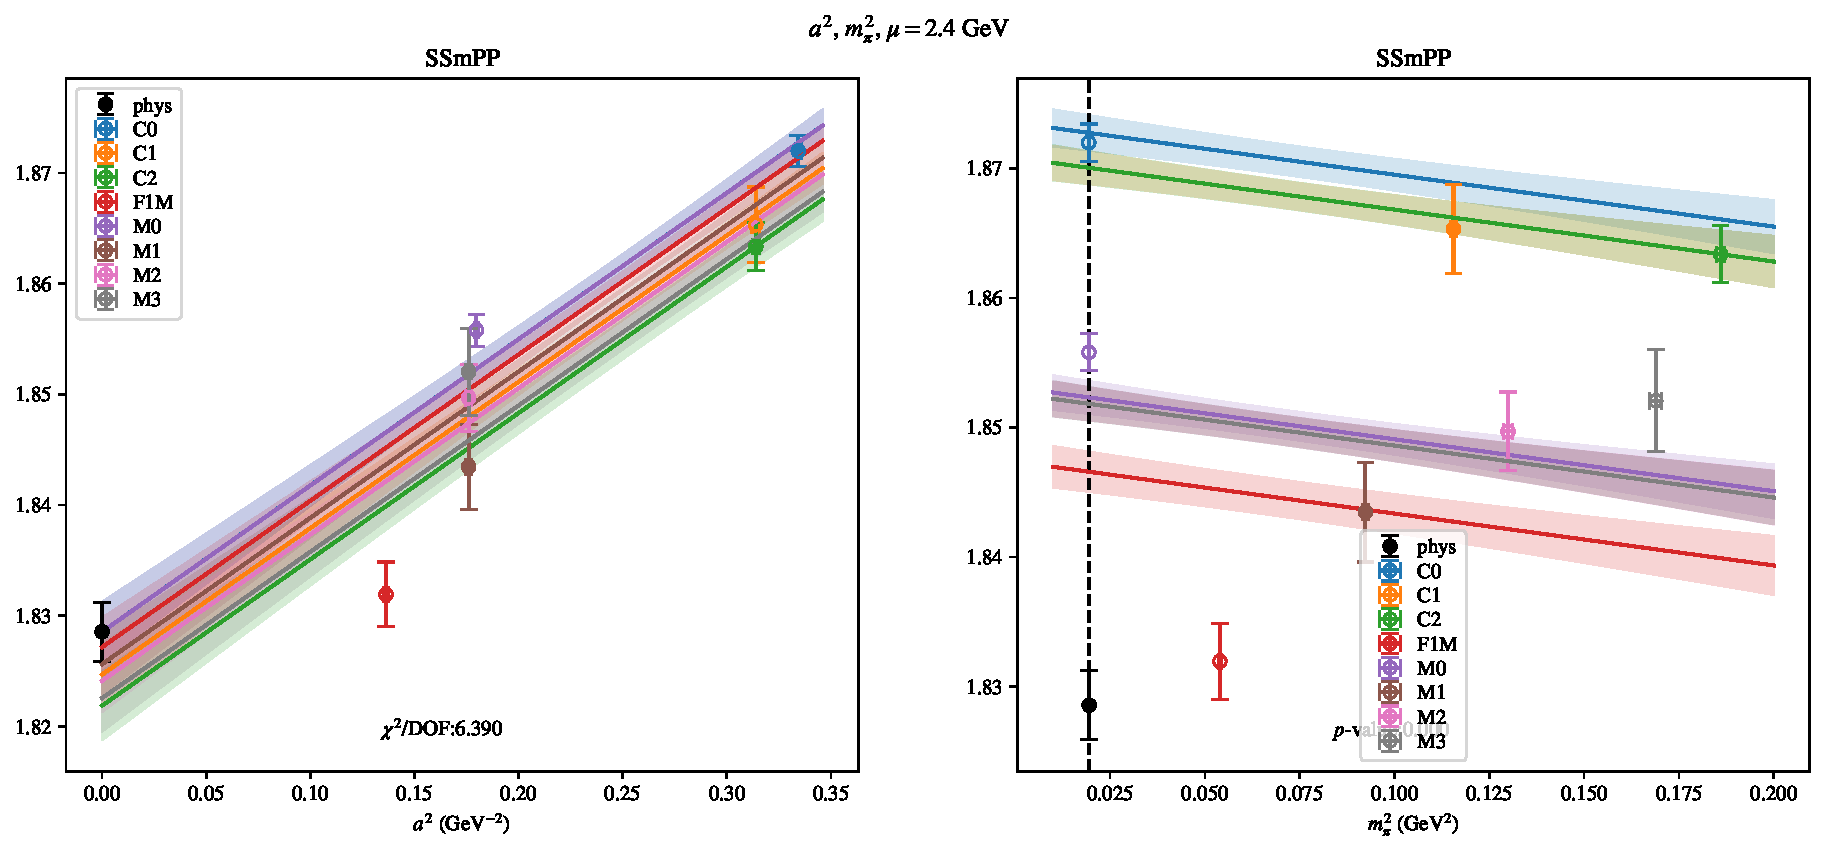
\includepdf[link, pages=-]{SSmPP/NPR/a2m2_24.pdf}
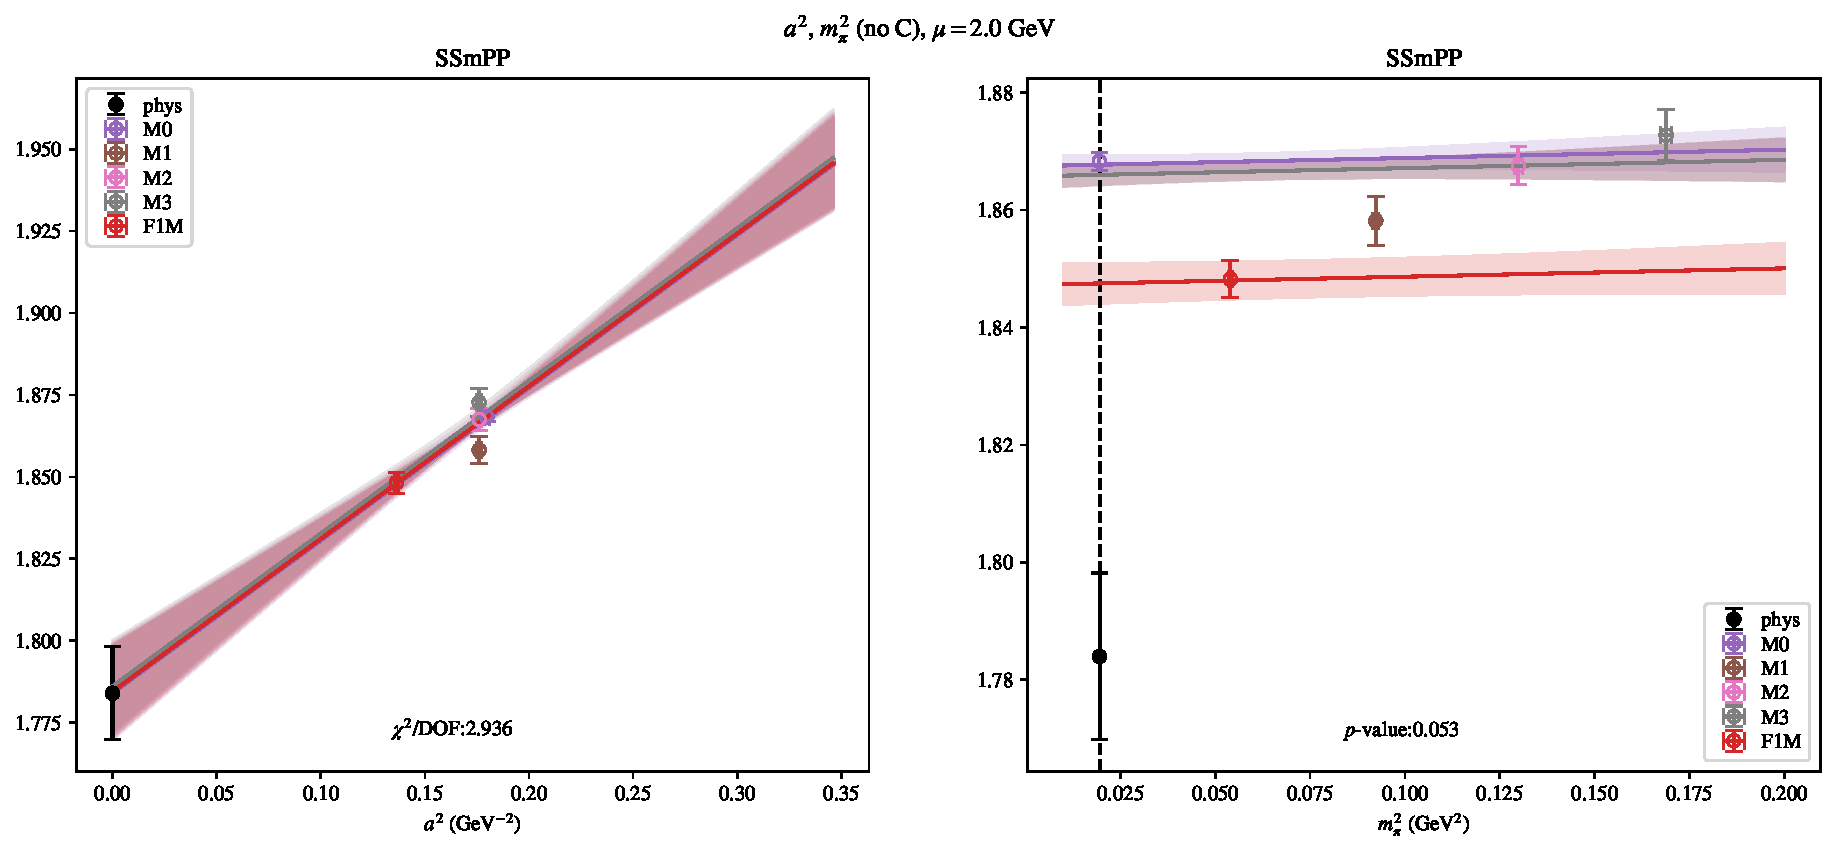
\includepdf[link, pages=-]{SSmPP/NPR/a2m2noC_20.pdf}
\includepdf[link, pages=-]{SSmPP/NPR/a2m2noC_22.pdf}
\includepdf[link, pages=-]{SSmPP/NPR/a2m2noC_23.pdf}
\includepdf[link, pages=-]{SSmPP/NPR/a2m2noC_24.pdf}
\includepdf[link, pages=-]{SSmPP/NPR/a2a4m2_20.pdf}
\includepdf[link, pages=-]{SSmPP/NPR/a2a4m2_22.pdf}
\includepdf[link, pages=-]{SSmPP/NPR/a2a4m2_23.pdf}
\includepdf[link, pages=-]{SSmPP/NPR/a2a4m2_24.pdf}
\includepdf[link, pages=-]{SSmPP/NPR/a2m2mcut_20.pdf}
\includepdf[link, pages=-]{SSmPP/NPR/a2m2mcut_22.pdf}
\includepdf[link, pages=-]{SSmPP/NPR/a2m2mcut_23.pdf}
\includepdf[link, pages=-]{SSmPP/NPR/a2m2mcut_24.pdf}
\includepdf[link, pages=-]{SSmPP/NPR/a2m2m4_20.pdf}
\includepdf[link, pages=-]{SSmPP/NPR/a2m2m4_22.pdf}
\includepdf[link, pages=-]{SSmPP/NPR/a2m2m4_23.pdf}
\includepdf[link, pages=-]{SSmPP/NPR/a2m2m4_24.pdf}
\clearpage
\section{$B_4$}
\begin{table}[h!]
\begin{center}
\begin{tabular}{|c|c|c|c|c|c|}
\hline
$\mu$ (GeV) & $a^2$, $m_\pi^2$& $a^2$, $m_\pi^2$ (no C)& $a^2$, $a^4$, $m_\pi^2$& $a^2$, $m_\pi^2$ (no M3, C2)& $a^2$, $m_\pi^2$, $m_\pi^4$\\
\hline
2.0& \hyperlink{SSpPP/NPR/a2m2_20.pdf.1}{\textbf{0.56711(94)}: 5.155 (0.0)} & \hyperlink{SSpPP/NPR/a2m2noC_20.pdf.1}{\textbf{0.5919(54)}: 0.934 (0.393)} & \hyperlink{SSpPP/NPR/a2a4m2_20.pdf.1}{\textbf{0.5997(87)}: 3.111 (0.014)} & \hyperlink{SSpPP/NPR/a2m2mcut_20.pdf.1}{\textbf{0.5668(10)}: 7.311 (0.0)} & \hyperlink{SSpPP/NPR/a2m2m4_20.pdf.1}{\textbf{0.5658(10)}: 4.514 (0.001)}\\
2.2& \hyperlink{SSpPP/NPR/a2m2_22.pdf.1}{\textbf{0.55003(96)}: 5.515 (0.0)} & \hyperlink{SSpPP/NPR/a2m2noC_22.pdf.1}{\textbf{0.5735(52)}: 1.315 (0.268)} & \hyperlink{SSpPP/NPR/a2a4m2_22.pdf.1}{\textbf{0.5766(86)}: 4.635 (0.001)} & \hyperlink{SSpPP/NPR/a2m2mcut_22.pdf.1}{\textbf{0.5499(10)}: 7.12 (0.0)} & \hyperlink{SSpPP/NPR/a2m2m4_22.pdf.1}{\textbf{0.54879(99)}: 4.735 (0.001)}\\
2.3& \hyperlink{SSpPP/NPR/a2m2_23.pdf.1}{\textbf{0.54271(92)}: 5.479 (0.0)} & \hyperlink{SSpPP/NPR/a2m2noC_23.pdf.1}{\textbf{0.5658(52)}: 1.442 (0.236)} & \hyperlink{SSpPP/NPR/a2a4m2_23.pdf.1}{\textbf{0.5690(85)}: 4.496 (0.001)} & \hyperlink{SSpPP/NPR/a2m2mcut_23.pdf.1}{\textbf{0.54261(97)}: 7.207 (0.0)} & \hyperlink{SSpPP/NPR/a2m2m4_23.pdf.1}{\textbf{0.54154(97)}: 4.8 (0.001)}\\
2.4& \hyperlink{SSpPP/NPR/a2m2_24.pdf.1}{\textbf{0.53684(91)}: 5.295 (0.0)} & \hyperlink{SSpPP/NPR/a2m2noC_24.pdf.1}{\textbf{0.5576(51)}: 1.384 (0.251)} & \hyperlink{SSpPP/NPR/a2a4m2_24.pdf.1}{\textbf{0.5584(83)}: 4.966 (0.001)} & \hyperlink{SSpPP/NPR/a2m2mcut_24.pdf.1}{\textbf{0.53686(97)}: 7.011 (0.0)} & \hyperlink{SSpPP/NPR/a2m2m4_24.pdf.1}{\textbf{0.53575(97)}: 4.991 (0.001)}\\
\hline
\end{tabular}
\caption{Physical point value from chiral and continuum extrapolation at renormalisation scale $\mu$. Entries are \textbf{value(error)}: $\chi^2/\text{DOF}$ ($p$-value).}
\end{center}
\end{table}
\begin{table}[h!]
\begin{center}
\begin{tabular}{|c c|c|c|c|c|c|}
\hline
$\mu$ (GeV) &  & $a^2$, $m_\pi^2$& $a^2$, $m_\pi^2$ (no C)& $a^2$, $a^4$, $m_\pi^2$& $a^2$, $m_\pi^2$ (no M3, C2)& $a^2$, $m_\pi^2$, $m_\pi^4$\\
\hline
\multirow{2}{0.5in}{2.0} & $\alpha$ & 0.2684(65)& 0.016(53)& -0.2(12)& 0.2693(70)& 0.2762(70)\\
 & $\beta$ & 0.00768(17)& 0.00709(26)& 0.00744(17)& 0.00810(28)& 0.01003(71)\\
\hline
\multirow{2}{0.5in}{2.2} & $\alpha$ & 0.3012(70)& 0.055(53)& -0.1(13)& 0.3011(74)& 0.3090(73)\\
 & $\beta$ & 0.00738(15)& 0.00670(24)& 0.00719(15)& 0.00787(27)& 0.00980(74)\\
\hline
\multirow{2}{0.5in}{2.3} & $\alpha$ & 0.3187(71)& 0.074(53)& -0.1(13)& 0.3186(74)& 0.3262(74)\\
 & $\beta$ & 0.00734(15)& 0.00667(24)& 0.00715(15)& 0.00778(27)& 0.00964(73)\\
\hline
\multirow{2}{0.5in}{2.4} & $\alpha$ & 0.3313(71)& 0.108(54)& -0.026& 0.3304(75)& 0.3384(75)\\
 & $\beta$ & 0.00734(14)& 0.00665(22)& 0.00718(14)& 0.00770(24)& 0.00932(70)\\
\hline
\end{tabular}
\caption{Fit values of coefficients in $B = B_{phys} + \mathbf{\alpha} a^2 + \mathbf{\beta}\left(\frac{m_\pi^2}{f_\pi^2}-\frac{m_{\pi,PDG}^2}{f_\pi^2}\right) + \ldots$.}
\end{center}
\end{table}
\includepdf[link, pages=-]{SSpPP/NPR/a2m2_20.pdf}
\includepdf[link, pages=-]{SSpPP/NPR/a2m2_22.pdf}
\includepdf[link, pages=-]{SSpPP/NPR/a2m2_23.pdf}
\includepdf[link, pages=-]{SSpPP/NPR/a2m2_24.pdf}
\includepdf[link, pages=-]{SSpPP/NPR/a2m2noC_20.pdf}
\includepdf[link, pages=-]{SSpPP/NPR/a2m2noC_22.pdf}
\includepdf[link, pages=-]{SSpPP/NPR/a2m2noC_23.pdf}
\includepdf[link, pages=-]{SSpPP/NPR/a2m2noC_24.pdf}
\includepdf[link, pages=-]{SSpPP/NPR/a2a4m2_20.pdf}
\includepdf[link, pages=-]{SSpPP/NPR/a2a4m2_22.pdf}
\includepdf[link, pages=-]{SSpPP/NPR/a2a4m2_23.pdf}
\includepdf[link, pages=-]{SSpPP/NPR/a2a4m2_24.pdf}
\includepdf[link, pages=-]{SSpPP/NPR/a2m2mcut_20.pdf}
\includepdf[link, pages=-]{SSpPP/NPR/a2m2mcut_22.pdf}
\includepdf[link, pages=-]{SSpPP/NPR/a2m2mcut_23.pdf}
\includepdf[link, pages=-]{SSpPP/NPR/a2m2mcut_24.pdf}
\includepdf[link, pages=-]{SSpPP/NPR/a2m2m4_20.pdf}
\includepdf[link, pages=-]{SSpPP/NPR/a2m2m4_22.pdf}
\includepdf[link, pages=-]{SSpPP/NPR/a2m2m4_23.pdf}
\includepdf[link, pages=-]{SSpPP/NPR/a2m2m4_24.pdf}
\clearpage
\section{$B_5$}
\begin{table}[h!]
\begin{center}
\begin{tabular}{|c|c|c|c|c|c|}
\hline
$\mu$ (GeV) & $a^2$, $m_\pi^2$& $a^2$, $m_\pi^2$ (no C)& $a^2$, $a^4$, $m_\pi^2$& $a^2$, $m_\pi^2$ (no M3, C2)& $a^2$, $m_\pi^2$, $m_\pi^4$\\
\hline
2.0& \hyperlink{TT/NPR/a2m2_20.pdf.1}{\textbf{1.5365(50)}: 7.108 (0.0)} & \hyperlink{TT/NPR/a2m2noC_20.pdf.1}{\textbf{1.646(14)}: 1.437 (0.238)} & \hyperlink{TT/NPR/a2a4m2_20.pdf.1}{\textbf{1.718(23)}: 1.823 (0.121)} & \hyperlink{TT/NPR/a2m2mcut_20.pdf.1}{\textbf{1.5342(49)}: 10.979 (0.0)} & \hyperlink{TT/NPR/a2m2m4_20.pdf.1}{\textbf{1.5294(49)}: 6.645 (0.0)}\\
2.2& \hyperlink{TT/NPR/a2m2_22.pdf.1}{\textbf{1.3997(50)}: 6.636 (0.0)} & \hyperlink{TT/NPR/a2m2noC_22.pdf.1}{\textbf{1.509(14)}: 1.143 (0.319)} & \hyperlink{TT/NPR/a2a4m2_22.pdf.1}{\textbf{1.560(23)}: 2.668 (0.03)} & \hyperlink{TT/NPR/a2m2mcut_22.pdf.1}{\textbf{1.3982(49)}: 9.808 (0.0)} & \hyperlink{TT/NPR/a2m2m4_22.pdf.1}{\textbf{1.3939(47)}: 6.083 (0.0)}\\
2.3& \hyperlink{TT/NPR/a2m2_23.pdf.1}{\textbf{1.3431(45)}: 7.834 (0.0)} & \hyperlink{TT/NPR/a2m2noC_23.pdf.1}{\textbf{1.453(13)}: 1.046 (0.351)} & \hyperlink{TT/NPR/a2a4m2_23.pdf.1}{\textbf{1.509(21)}: 2.449 (0.044)} & \hyperlink{TT/NPR/a2m2mcut_23.pdf.1}{\textbf{1.3414(43)}: 11.754 (0.0)} & \hyperlink{TT/NPR/a2m2m4_23.pdf.1}{\textbf{1.3375(42)}: 7.202 (0.0)}\\
2.4& \hyperlink{TT/NPR/a2m2_24.pdf.1}{\textbf{1.2987(43)}: 6.997 (0.0)} & \hyperlink{TT/NPR/a2m2noC_24.pdf.1}{\textbf{1.393(12)}: 0.986 (0.373)} & \hyperlink{TT/NPR/a2a4m2_24.pdf.1}{\textbf{1.435(20)}: 3.057 (0.016)} & \hyperlink{TT/NPR/a2m2mcut_24.pdf.1}{\textbf{1.2975(42)}: 10.515 (0.0)} & \hyperlink{TT/NPR/a2m2m4_24.pdf.1}{\textbf{1.2933(41)}: 6.619 (0.0)}\\
\hline
\end{tabular}
\caption{Physical point value from chiral and continuum extrapolation at renormalisation scale $\mu$. Entries are \textbf{value(error)}: $\chi^2/\text{DOF}$ ($p$-value).}
\end{center}
\end{table}
\begin{table}[h!]
\begin{center}
\begin{tabular}{|c c|c|c|c|c|c|}
\hline
$\mu$ (GeV) &  & $a^2$, $m_\pi^2$& $a^2$, $m_\pi^2$ (no C)& $a^2$, $a^4$, $m_\pi^2$& $a^2$, $m_\pi^2$ (no M3, C2)& $a^2$, $m_\pi^2$, $m_\pi^4$\\
\hline
\multirow{2}{0.5in}{2.0} & $\alpha$ & -0.392(54)& -0.76(44)& -1.3(10)& -0.389(58)& -0.381(56)\\
 & $\beta$ & 0.00685(17)& 0.00677(25)& 0.00664(15)& 0.00738(26)& 0.01031(64)\\
\hline
\multirow{2}{0.5in}{2.2} & $\alpha$ & -0.341(62)& -0.74(44)& -1.2(10)& -0.340(64)& -0.331(62)\\
 & $\beta$ & 0.00667(14)& 0.00627(22)& 0.00646(12)& 0.00726(25)& 0.00995(68)\\
\hline
\multirow{2}{0.5in}{2.3} & $\alpha$ & -0.315(63)& -0.73(44)& -1.2(10)& -0.312(63)& -0.304(61)\\
 & $\beta$ & 0.00663(17)& 0.00626(25)& 0.00639(14)& 0.00723(28)& 0.01016(71)\\
\hline
\multirow{2}{0.5in}{2.4} & $\alpha$ & -0.301(63)& -0.68(45)& -1.1(10)& -0.299(66)& -0.290(64)\\
 & $\beta$ & 0.00664(13)& 0.00623(20)& 0.00647(12)& 0.00714(23)& 0.00964(64)\\
\hline
\end{tabular}
\caption{Fit values of coefficients in $B = B_{phys} + \mathbf{\alpha} a^2 + \mathbf{\beta}\left(\frac{m_\pi^2}{f_\pi^2}-\frac{m_{\pi,PDG}^2}{f_\pi^2}\right) + \ldots$.}
\end{center}
\end{table}
\includepdf[link, pages=-]{TT/NPR/a2m2_20.pdf}
\includepdf[link, pages=-]{TT/NPR/a2m2_22.pdf}
\includepdf[link, pages=-]{TT/NPR/a2m2_23.pdf}
\includepdf[link, pages=-]{TT/NPR/a2m2_24.pdf}
\includepdf[link, pages=-]{TT/NPR/a2m2noC_20.pdf}
\includepdf[link, pages=-]{TT/NPR/a2m2noC_22.pdf}
\includepdf[link, pages=-]{TT/NPR/a2m2noC_23.pdf}
\includepdf[link, pages=-]{TT/NPR/a2m2noC_24.pdf}
\includepdf[link, pages=-]{TT/NPR/a2a4m2_20.pdf}
\includepdf[link, pages=-]{TT/NPR/a2a4m2_22.pdf}
\includepdf[link, pages=-]{TT/NPR/a2a4m2_23.pdf}
\includepdf[link, pages=-]{TT/NPR/a2a4m2_24.pdf}
\includepdf[link, pages=-]{TT/NPR/a2m2mcut_20.pdf}
\includepdf[link, pages=-]{TT/NPR/a2m2mcut_22.pdf}
\includepdf[link, pages=-]{TT/NPR/a2m2mcut_23.pdf}
\includepdf[link, pages=-]{TT/NPR/a2m2mcut_24.pdf}
\includepdf[link, pages=-]{TT/NPR/a2m2m4_20.pdf}
\includepdf[link, pages=-]{TT/NPR/a2m2m4_22.pdf}
\includepdf[link, pages=-]{TT/NPR/a2m2m4_23.pdf}
\includepdf[link, pages=-]{TT/NPR/a2m2m4_24.pdf}
\clearpage
\end{document}